\documentclass[11pt,a4paper,twoside]{book}
\usepackage[T1]{fontenc}
\usepackage[utf8]{inputenc}
\usepackage{mathpazo}
\usepackage[scaled=0.90]{helvet}
\usepackage{courier}
\usepackage[a4paper,inner=3.0cm,outer=2.4cm,top=2.6cm,bottom=2.8cm]{geometry}
\usepackage{xcolor}
\usepackage{mathtools}
\usepackage{colortbl}
\usepackage{tikz}
\usetikzlibrary{calc,positioning,arrows.meta,decorations.pathmorphing}
\usepackage{booktabs}
\usepackage{array}
\usepackage{longtable}
\usepackage{enumitem}
\usepackage[german=quotes]{csquotes}
\usepackage{fancyhdr}
\usepackage{titlesec}
\usepackage{amsmath,amssymb}
\usepackage{tcolorbox}
\tcbuselibrary{skins,breakable}
\usepackage[hidelinks]{hyperref}

\definecolor{tief}{HTML}{1F3A5F}
\definecolor{mittel}{HTML}{2E5F8A}
\definecolor{akzent}{HTML}{A34A28}
\definecolor{sand}{HTML}{F4F1EA}
\definecolor{grau}{HTML}{5A5A5A}
\definecolor{gruen}{HTML}{2F6B4F}
\definecolor{purpur}{HTML}{5B3A72}

\newcolumntype{P}[1]{>{\raggedright\arraybackslash}p{#1}}

\newcommand{\kursiv}[1]{{\itshape\color{grau}#1}}
\newcommand{\code}[1]{{\ttfamily\small #1}}
\newcommand{\Person}[1]{\textbf{#1}}
\newcommand{\Begriff}[1]{\textbf{#1}}
\newcommand{\zit}[1]{\textsuperscript{[#1]}}
\newcommand{\Oh}{\mathcal{O}}
\newcommand{\boxtitel}[1]{{\bfseries\color{tief}#1}\par\vspace{6pt}}
\newcommand{\boxtitelr}[1]{{\bfseries\color{akzent}#1}\par\vspace{6pt}}
\newcommand{\boxtitelg}[1]{{\bfseries\color{gruen}#1}\par\vspace{6pt}}
\newcommand{\boxtitelp}[1]{{\bfseries\color{purpur}#1}\par\vspace{6pt}}
\newcommand{\boxtitelm}[1]{{\bfseries\color{mittel}#1}\par\vspace{6pt}}
\newcommand{\loesung}{\par\vspace{8pt}{\bfseries\color{mittel}Lösung}\par\vspace{4pt}}
\newcommand{\schritt}[1]{\par\vspace{5pt}{\bfseries\color{grau}#1}\par\vspace{2pt}}

% Graphentheoretische Notation
\newcommand{\Gr}{G}
\newcommand{\Kn}[1]{K_{#1}}
\newcommand{\Kmn}[2]{K_{#1,#2}}
\newcommand{\Grad}{\deg}
\newcommand{\Nb}{N}
\newcommand{\chrom}{\chi}
\newcommand{\Ecken}{V}
\newcommand{\Kanten}{E}

\newtcolorbox{grundbox}[1][tief]{
  breakable, enhanced, colback=sand, colframe=sand,
  boxrule=0pt, leftrule=3pt, borderline west={3pt}{0pt}{#1},
  left=12pt, right=10pt, top=10pt, bottom=10pt,
  sharp corners, before skip=12pt, after skip=12pt}

\newenvironment{merksatz}{\begin{grundbox}[tief]}{\end{grundbox}}
\newenvironment{warnung}{\begin{grundbox}[akzent]}{\end{grundbox}}
\newenvironment{definition}{\begin{grundbox}[mittel]}{\end{grundbox}}
\newenvironment{geschichte}{\begin{grundbox}[gruen]}{\end{grundbox}}
\newenvironment{forschung}{\begin{grundbox}[purpur]}{\end{grundbox}}
\newenvironment{aufgabe}{\begin{grundbox}[grau]}{\end{grundbox}}
\newenvironment{technik}{\begin{grundbox}[mittel]}{\end{grundbox}}

\titleformat{\chapter}[display]
  {\normalfont\huge\bfseries\color{tief}}{\Large\color{grau}Kapitel \thechapter}{8pt}{\Huge}
\titleformat{\part}[display]
  {\normalfont\huge\bfseries\color{tief}\filcenter}{\Large\color{grau}Teil \thepart}{10pt}{\Huge}
\titlespacing*{\chapter}{0pt}{10pt}{28pt}

\pagestyle{fancy}
\fancyhf{}
\fancyhead[LE,LO]{\small\itshape\color{grau}\leftmark}
\fancyfoot[LE,LO]{\small\color{grau}\thepage}
\renewcommand{\headrulewidth}{0.4pt}
\renewcommand{\footrulewidth}{0pt}
\renewcommand{\chaptermark}[1]{\markboth{#1}{}}
\setlength{\parindent}{0pt}
\setlength{\parskip}{6pt}
\renewcommand{\arraystretch}{1.3}

\renewcommand{\contentsname}{Inhaltsverzeichnis}
\renewcommand{\chaptername}{Kapitel}
\renewcommand{\partname}{Teil}
\renewcommand{\appendixname}{Anhang}
\renewcommand{\tablename}{Tabelle}
\renewcommand{\figurename}{Abbildung}

\hyphenation{Öko-no-me-trie öko-no-me-trisch En-do-ge-ni-tät
In-stru-ment-va-ri-a-ble Si-mul-ta-ni-tät Iden-ti-fi-ka-ti-on Pa-nel-da-ten
Ko-in-te-gra-ti-on Ein-heits-wur-zel Vek-tor-au-to-re-gres-si-on
Zu-zah-lung Arzt-be-su-che Preis-elas-ti-zi-tät Mo-men-ten-me-tho-de
Ir-rfahrt Mar-kow-Ket-te Über-gangs-ma-trix sta-tio-när
Brown-sche Brown-schen Mar-tin-gal Mar-tin-ga-le Stopp-zeit Stopp-zei-ten
Pois-son-Pro-zess Ver-zwei-gungs-pro-zess Fil-tra-ti-on Pfad-ei-gen-schaft
Dif-fu-si-on Dif-fu-si-o-nen Wie-ner-Pro-zess Ar-kus-si-nus-Ge-setz
Ent-schei-dung Ent-schei-dun-gen Nut-zen-funk-ti-on Ri-si-ko-aver-si-on
An-ti-ko-agu-la-ti-on Vor-hof-flim-mern Schlag-an-fall Blu-tungs-ri-si-ko
Er-war-tungs-nut-zen Si-cher-heits-äqui-va-lent Ent-schei-dungs-baum
Schwel-len-wert Mar-kow-Mo-dell Dis-kon-tie-rung Prio-ri-sie-rung
Kau-sa-li-tät kau-sa-le kau-sa-len Stör-grö-ße Stör-grö-ßen Kol-li-der
Me-di-a-tor Me-di-a-ti-on Hin-ter-tür-test Rando-mi-sie-rung rando-mi-siert
In-stru-ment-va-ri-a-ble Ziel-stu-di-en-emu-la-ti-on Stan-dar-di-sie-rung
Kon-tra-fak-tisch kon-tra-fak-ti-sche Be-hand-lungs-ef-fekt Neu-stadt Kli-ni-kum
Sep-sis An-ti-bio-ti-ka-ga-be Be-ob-ach-tungs-da-ten Be-ob-ach-tungs-äqui-va-lenz
Pro-pen-si-ty Ge-wich-tung Schwe-re-grad}

\tikzset{
  knoten/.style={circle, fill=tief, inner sep=0pt, minimum size=5.5pt},
  knotenb/.style={circle, draw=tief, fill=white, line width=0.9pt, inner sep=1pt, minimum size=15pt, font=\scriptsize},
  knotenr/.style={circle, draw=akzent, fill=akzent!12, line width=0.9pt, inner sep=1pt, minimum size=15pt, font=\scriptsize},
  knoteng/.style={circle, draw=gruen, fill=gruen!12, line width=0.9pt, inner sep=1pt, minimum size=15pt, font=\scriptsize},
  kante/.style={draw=grau, line width=0.9pt},
  kanted/.style={draw=akzent, line width=1.5pt},
}

\newcommand{\MW}{\overline{x}}
\newcommand{\dd}{\mathrm{d}}
\newcommand{\R}{\mathbb{R}}
\newcommand{\Z}{\mathbb{Z}}
\newcommand{\Ent}{H}
\newcommand{\vek}[1]{\boldsymbol{#1}}
\newcommand{\lb}{\operatorname{ld}}



\newcommand{\Risk}{\mathcal{R}}
\newcommand{\Hyp}{\mathcal{H}}
\newcommand{\E}{\mathbb{E}}

\newcommand{\dops}{\operatorname{do}}

\begin{document}
\frontmatter
\begin{titlepage}
\centering
\vspace*{1.6cm}
{\footnotesize\scshape\color{grau} Mathematik von Grund auf --- Band 26}\\[2.0cm]
{\Huge\bfseries\color{tief} Wenn die Daten sich\\[6pt] selbst bestimmen}\\[16pt]
{\Large\color{akzent} Ökonometrie}\\[1.5cm]

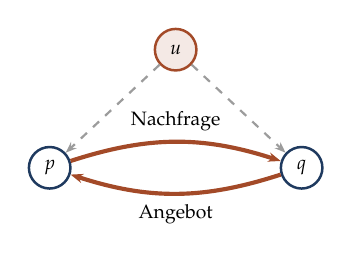
\begin{tikzpicture}[scale=1.0, every node/.style={font=\small}]
\node[knotenb] (p) at (-1.6,0) {$p$};
\node[knotenb] (q) at (1.6,0) {$q$};
\node[knotenr] (u) at (0,1.5) {$u$};
\draw[kanted, -{Stealth[length=4.5pt]}] (p) to[bend left=18] node[above]{\scriptsize Nachfrage} (q);
\draw[kanted, -{Stealth[length=4.5pt]}] (q) to[bend left=18] node[below]{\scriptsize Angebot} (p);
\draw[grau!60, line width=0.8pt, dashed, -{Stealth[length=4pt]}] (u)--(p);
\draw[grau!60, line width=0.8pt, dashed, -{Stealth[length=4pt]}] (u)--(q);
\end{tikzpicture}

\vspace{1.4cm}
{\large\color{grau} Von der Simultanität bis zur Kointegration}\\[6pt]
{\color{grau} Jeder Schritt erklärt. Mit vollständig durchgerechneten Übungsaufgaben.}\\[1.9cm]
{\small\color{grau} Stand der Forschung: August 2026}
\end{titlepage}
\thispagestyle{empty}
\vspace*{\fill}
\begin{flushleft}
{\small\color{grau}
\textbf{\color{tief}Mathematik von Grund auf} --- Band 26\\[2pt]
\textit{Wenn die Daten sich selbst bestimmen} $\cdot$ Ökonometrie\\[14pt]

Herausgeber und Urheber: Jürgen Maier\\[2pt]
Entstanden 2026 in Zusammenarbeit mit Claude (Anthropic); Konzeption, Vorgaben, Prüfung und Herausgeberschaft: Jürgen Maier.\\[14pt]

\textbf{Lizenz}\\[2pt]
Dieses Werk ist lizenziert unter einer Creative-Commons-Lizenz \textbf{Namensnennung -- Weitergabe unter gleichen Bedingungen 4.0 International (CC BY-SA 4.0)}. Sie dürfen das Werk vervielfältigen, verbreiten, bearbeiten und auch kommerziell nutzen, sofern Sie den Urheber nennen und Bearbeitungen unter derselben Lizenz weitergeben.\\[2pt]
Lizenztext: \texttt{https://creativecommons.org/licenses/by-sa/4.0/legalcode.de}\\[14pt]

\textbf{Quellen und Fassungen}\\[2pt]
Quelltexte, Simulationen, Fehlermeldungen und aktuelle Fassungen aller Bände:\\
\texttt{https://github.com/juergenmaier2026/mathematik-von-grund-auf}\\[2pt]
Dauerhaft archiviert bei Zenodo: \texttt{https://doi.org/10.5281/zenodo.23698547}\\[14pt]

\textbf{Zitiervorschlag}\\[2pt]
Maier, J. (2026). \textit{Mathematik von Grund auf, Band 26: Wenn die Daten sich selbst bestimmen}. Fassung 1.0.1. \texttt{https://doi.org/10.5281/zenodo.23698547}\\[14pt]

Satz: \LaTeX{} mit Palatino. Fassung 1.0.1, Oktober 2026. 156 Seiten.
}
\end{flushleft}
\vspace*{1.5cm}

\tableofcontents
\mainmatter

\chapter*{Vorwort}
\addcontentsline{toc}{chapter}{Vorwort}

\begin{merksatz}
\boxtitel{Was dieser Band von Band 17 unterscheidet}
Die Statistik aus Band 17 nahm an, dass die erklärenden Größen gegeben sind und die Störungen unabhängig von ihnen. In den Daten, mit denen Volkswirte arbeiten, ist beides regelmäßig falsch.

\begin{center}
{\small
\renewcommand{\arraystretch}{1.52}
\begin{tabular}{@{}P{2.4cm}P{6.2cm}@{}}
\toprule
\textbf{Preise} & entstehen aus Angebot \kursiv{und} Nachfrage --- sie erklären die Menge und werden von ihr erklärt.\\
\textbf{Verträge} & werden gewählt, nicht zugeteilt --- wer viel zum Arzt geht, wählt einen anderen Tarif.\\
\textbf{Erwartungen} & richten sich nach der Politik, die man untersuchen will.\\
\bottomrule
\end{tabular}}
\end{center}

\begin{center}
\begin{minipage}{0.9\textwidth}
\textbf{Die Daten entstehen durch Entscheidungen derer, die man untersucht. Das ist der Gegenstand dieses Bandes.}
\end{minipage}
\end{center}
\end{merksatz}

\begin{merksatz}
\boxtitel{Wo der Band steht}
\begin{center}
{\small
\renewcommand{\arraystretch}{1.5}
\begin{tabular}{@{}P{2.2cm}P{6.4cm}@{}}
\toprule
\textbf{Band 17} & schätzt und testet, bei gegebenen Merkmalen.\\
\textbf{Band 22} & sagt vorher, ohne nach Ursachen zu fragen.\\
\textbf{Band 23} & klärt, wann ein Zusammenhang ursächlich ist.\\
\textbf{Band 25} & liefert die Prozesse, aus denen Zeitreihen bestehen.\\
\textbf{Hier} & werden alle vier gebraucht --- und zwar gleichzeitig.\\
\bottomrule
\end{tabular}}
\end{center}

\begin{center}
\begin{minipage}{0.88\textwidth}
\kursiv{\textbf{Die Ökonometrie ist kein eigenes Gebiet neben diesen, sondern ihre Verbindung unter erschwerten Bedingungen}: kausale Fragen, Beobachtungsdaten, rückgekoppelte Systeme und Zeitreihen, die selten stationär sind. Sie hat dafür eigene Begriffe entwickelt, die in den Nachbarfächern fehlen --- allen voran die Identifikation.}
\end{minipage}
\end{center}
\end{merksatz}

\begin{merksatz}
\boxtitel{Drei Ergebnisse, die man nicht erwartet}
\begin{center}
{\small
\renewcommand{\arraystretch}{1.55}
\begin{tabular}{@{}P{1.0cm}P{7.4cm}@{}}
\toprule
$1$ & Aus Preis- und Mengendaten allein lässt sich \kursiv{weder} die Nachfrage- \kursiv{noch} die Angebotskurve bestimmen --- gleich wie viele Beobachtungen man hat. \kursiv{(Kapitel 2)}\\
$2$ & Zwei voneinander völlig unabhängige Zeitreihen zeigen in den meisten Fällen einen hochsignifikanten Zusammenhang. \kursiv{(Kapitel 11)}\\
$3$ & Ein Modell, das die Vergangenheit gut beschreibt, kann gerade deshalb für die Beurteilung einer Politikänderung untauglich sein. \kursiv{(Kapitel 13)}\\
\bottomrule
\end{tabular}}
\end{center}

\begin{center}
\begin{minipage}{0.88\textwidth}
\kursiv{Das zweite Ergebnis ist das folgenreichste. \textbf{Bei nichtstationären Reihen liegt der Anteil scheinbar bedeutsamer Zusammenhänge bei über siebzig Prozent} --- nicht bei fünf. Jede Zeitreihenauswertung, die das übersieht, produziert Befunde am laufenden Band.}
\end{minipage}
\end{center}
\end{merksatz}

\begin{merksatz}
\boxtitel{Die sechs Teile}
\begin{center}
{\small
\renewcommand{\arraystretch}{1.5}
\begin{tabular}{@{}P{1.4cm}P{3.6cm}P{3.0cm}@{}}
\toprule
\textbf{Teil} & \textbf{Thema} & \textbf{Kapitel}\\
\midrule
I & Das Problem & $1$--$3$\\
II & Querschnittsdaten & $4$--$6$\\
III & Dieselben über die Zeit & $7$--$9$\\
IV & Zeitreihen & $10$--$12$\\
V & Vorhersage und Politik & $13$--$14$\\
VI & Stand & $15$\\
\bottomrule
\end{tabular}}
\end{center}

\schritt{Der Leitfall}
Wie stark sinkt die Zahl der Arztbesuche, wenn Patienten zuzahlen müssen?

\begin{center}
\begin{minipage}{0.88\textwidth}
\kursiv{\textbf{Die Frage hat alle Eigenschaften, um die es hier geht}: Wer krank ist, wählt einen anderen Tarif; wer zuzahlt, geht seltener, aber vielleicht auch dann nicht, wenn er sollte; und die Zuzahlung wird politisch gesetzt, also nicht zufällig. Zugleich gibt es einen randomisierten Versuch, an dem sich alle Verfahren messen lassen --- das amerikanische Krankenversicherungsexperiment der 1970er Jahre.}
\end{minipage}
\end{center}
\end{merksatz}

\begin{warnung}
\boxtitelr{Drei Warnungen}
\begin{center}
{\small
\renewcommand{\arraystretch}{1.55}
\begin{tabular}{@{}P{2.2cm}P{6.4cm}@{}}
\toprule
\textbf{Erste} & Kein Schätzverfahren rettet eine Frage, die nicht identifiziert ist. Das ist eine Eigenschaft des Modells, nicht der Daten.\\
\textbf{Zweite} & Zeitreihen verleiten zu Befunden. Wer nicht auf Stationarität prüft, findet fast alles.\\
\textbf{Dritte} & Eine geschätzte Beziehung gilt für die Politik, unter der sie beobachtet wurde --- nicht notwendig für eine andere.\\
\bottomrule
\end{tabular}}
\end{center}

\begin{center}
\begin{minipage}{0.88\textwidth}
\kursiv{Die erste Warnung ist der eigentliche Beitrag der Ökonometrie zu den Nachbarfächern. \textbf{Identifikation fragt, ob eine Größe aus unbegrenzt vielen Daten überhaupt bestimmbar wäre} --- vor jeder Frage nach Schätzung, Streuung und Test. Band 23 stellte dieselbe Frage mit Graphen; hier wird sie mit Gleichungen gestellt.}
\end{minipage}
\end{center}
\end{warnung}

\begin{merksatz}
\boxtitel{Was dieser Band voraussetzt}
\begin{center}
{\small
\renewcommand{\arraystretch}{1.48}
\begin{tabular}{@{}P{3.0cm}P{1.6cm}P{3.0cm}@{}}
\toprule
\textbf{Werkzeug} & \textbf{Band} & \textbf{gebraucht in}\\
\midrule
Regression, Tests & $17$ & durchgehend\\
Matrizen & $2$ & Kapitel 2--4\\
Kausale Begriffe & $23$ & Kapitel 1--3, 9\\
Prozesse & $25$ & Kapitel 10--12\\
Lernverfahren & $22$ & Kapitel 14\\
\bottomrule
\end{tabular}}
\end{center}
\end{merksatz}

\part{Das Problem}

\chapter{Wenn der Regressor nicht unschuldig ist}

\section{Der Leitfall}

\begin{merksatz}
\boxtitel{Zuzahlung und Arztbesuche}
Eine Krankenkasse bietet Tarife mit verschiedenen Zuzahlungen an. In den Abrechnungsdaten findet sich:

\begin{center}
{\small
\renewcommand{\arraystretch}{1.5}
\begin{tabular}{@{}P{3.6cm}P{2.6cm}@{}}
\toprule
\textbf{Auswertung} & \textbf{je Euro Zuzahlung}\\
\midrule
schlichte Regression & $-0{,}376$ Besuche\\
\midrule
wahre Wirkung & $-0{,}100$ Besuche\\
\bottomrule
\end{tabular}}
\end{center}

\begin{center}
\begin{minipage}{0.9\textwidth}
\textbf{Die Auswertung überschätzt die Wirkung um das Vierfache --- und man sieht es den Daten nicht an.}
\end{minipage}
\end{center}

\schritt{Woran es liegt}
\begin{center}
\begin{minipage}{0.88\textwidth}
\kursiv{Wer selten krank ist, wählt den Tarif mit hoher Zuzahlung und niedrigem Beitrag. \textbf{Der Vergleich der Tarife vergleicht also auch Gesunde mit Kranken}, und ein Teil des Unterschieds in den Besuchszahlen stammt daher. In der Sprache von Band 23 ist der Gesundheitszustand eine Störgröße; in der Sprache dieses Bandes heißt die Zuzahlung \Begriff{endogen}.}
\end{minipage}
\end{center}
\end{merksatz}

\begin{definition}
\boxtitelm{Definition 1.1 --- exogen und endogen}
Im Modell $y = \beta x + u$ heißt $x$
\begin{center}
{\small
\renewcommand{\arraystretch}{1.5}
\begin{tabular}{@{}P{2.4cm}P{6.0cm}@{}}
\toprule
\textbf{exogen}, & wenn $\operatorname{Cov}(x,u) = 0$,\\
\textbf{endogen}, & sonst.\\
\bottomrule
\end{tabular}}
\end{center}
\end{definition}

\begin{merksatz}
\boxtitel{Satz 1.2 --- die Verzerrung der kleinsten Quadrate}
Für den Schätzer $\hat\beta$ gilt bei großem Stichprobenumfang
\[ \hat\beta \ \longrightarrow\ \beta + \frac{\operatorname{Cov}(x,u)}{\operatorname{Var}(x)} . \]

\schritt{Beweis}
\[ \hat\beta = \frac{\sum (x_i-\bar x)(y_i-\bar y)}{\sum(x_i-\bar x)^{2}} = \beta + \frac{\sum(x_i-\bar x)(u_i-\bar u)}{\sum(x_i-\bar x)^{2}} \]
Zähler und Nenner streben nach dem Gesetz der großen Zahlen gegen $\operatorname{Cov}(x,u)$ und $\operatorname{Var}(x)$. $\blacksquare$

\begin{center}
\begin{minipage}{0.9\textwidth}
\textbf{Die Verzerrung verschwindet nicht mit wachsendem Umfang --- mehr Daten machen das falsche Ergebnis nur genauer.}
\end{minipage}
\end{center}

\begin{center}
\begin{minipage}{0.88\textwidth}
\kursiv{\textbf{Das ist der Unterschied zwischen Verzerrung und Streuung in seiner unangenehmsten Form.} Bei zehn Millionen Versicherten liefert die Auswertung ein Vertrauensintervall von wenigen Tausendsteln um den falschen Wert. Die Statistik aus Band 17 meldet dabei nichts; sie prüft die Annahme nicht, auf der sie beruht.}
\end{minipage}
\end{center}

\schritt{Im Leitfall nachgerechnet}
\begin{center}
{\small
\renewcommand{\arraystretch}{1.48}
\begin{tabular}{@{}P{3.4cm}P{2.6cm}@{}}
\toprule
\textbf{Modell} & \textbf{Schätzung}\\
\midrule
nur Zuzahlung & $-0{,}376$\\
Zuzahlung und Gesundheit & $\mathbf{-0{,}098}$\\
\bottomrule
\end{tabular}}
\end{center}

\kursiv{Die zweite Zeile trifft --- aber nur, weil die Gesundheit in der Simulation beobachtbar ist. In Abrechnungsdaten ist sie es nicht.}
\end{merksatz}

\section{Drei Wege, wie Endogenität entsteht}

\begin{merksatz}
\boxtitel{Die Unterscheidung}
\begin{center}
{\small
\renewcommand{\arraystretch}{1.55}
\begin{tabular}{@{}P{2.8cm}P{5.8cm}@{}}
\toprule
\textbf{Ausgelassene Größe} & Eine Ursache beider Seiten fehlt im Modell --- die Störgröße aus Band 23.\\
\textbf{Simultanität} & $y$ wirkt auf $x$ zurück --- Preis und Menge.\\
\textbf{Messfehler} & $x$ ist fehlerhaft gemessen; der Fehler steckt dann in $u$.\\
\bottomrule
\end{tabular}}
\end{center}

\schritt{Der dritte Fall, gerechnet}
Wird $x$ mit unabhängigem Fehler der Varianz $\sigma_e^{2}$ gemessen, so gilt
\[ \hat\beta \ \longrightarrow\ \beta\cdot\frac{\sigma_x^{2}}{\sigma_x^{2}+\sigma_e^{2}} . \]

\begin{center}
{\small
\renewcommand{\arraystretch}{1.48}
\begin{tabular}{@{}P{2.8cm}P{2.0cm}P{2.6cm}@{}}
\toprule
\textbf{Zuverläs\-sigkeit} & \textbf{Faktor} & \textbf{Beispiel}\\
\midrule
$0{,}95$ & $0{,}95$ & Laborwert\\
$0{,}80$ & $0{,}80$ & Fragebogen\\
$0{,}50$ & $0{,}50$ & Erinnerung\\
\bottomrule
\end{tabular}}
\end{center}

\begin{center}
\begin{minipage}{0.9\textwidth}
\textbf{Messfehler im Regressor zieht den Koeffizienten immer zur Null --- Dämpfung, nicht Zufall.}
\end{minipage}
\end{center}

\begin{center}
\begin{minipage}{0.88\textwidth}
\kursiv{\textbf{Bei mehreren Regressoren gilt das nicht mehr}: Dort kann der Koeffizient des fehlerhaft gemessenen auch über den wahren Wert hinausgehen, und die Koeffizienten der genau gemessenen werden mitverzerrt. Das ist der Grund, warum \enquote{Kontrolle} für eine grob gemessene Störgröße nur teilweise wirkt --- Band 23, Kapitel~5.}
\end{minipage}
\end{center}
\end{merksatz}

\section{Der Maßstab}

\begin{merksatz}
\boxtitel{Wenn die Zuzahlung ausgelost wird}
Im amerikanischen Krankenversicherungsexperiment wurden Familien zufällig Tarifen zugewiesen. Die Simulation bildet das nach:

\begin{center}
{\small
\renewcommand{\arraystretch}{1.48}
\begin{tabular}{@{}P{2.4cm}P{2.6cm}@{}}
\toprule
\textbf{Zuzahlung} & \textbf{Besuche je Jahr}\\
\midrule
$0$ € & $8{,}01$\\
$10$ € & $7{,}00$\\
$20$ € & $5{,}99$\\
$30$ € & $5{,}02$\\
\bottomrule
\end{tabular}}
\end{center}
\[ \text{Steigung} = -0{,}0997 \quad\text{gegen den wahren Wert } -0{,}100 \]

\begin{center}
\begin{minipage}{0.9\textwidth}
\textbf{Das Los macht die Zuzahlung exogen --- und die schlichte Regression wird richtig.}
\end{minipage}
\end{center}

\begin{center}
\begin{minipage}{0.88\textwidth}
\kursiv{\textbf{Das wirkliche Experiment lief von 1974 bis 1982 mit rund $7700$ Teilnehmern} und kostete nach heutigem Geld etwa $400$ Millionen Dollar. Sein Hauptergebnis: Zuzahlungen senken die Inanspruchnahme deutlich, und zwar gleichermaßen bei nötigen und unnötigen Leistungen --- die Gesundheit der meisten Teilnehmer litt dennoch nicht messbar, die der ärmsten Kranken schon. Es ist bis heute der Maßstab, an dem sich jede Beobachtungsstudie zu dieser Frage messen lassen muss.}
\end{minipage}
\end{center}
\end{merksatz}

\section{Der Bruchfall}

\begin{warnung}
\boxtitelr{Warum man nicht einfach kontrolliert}
\begin{center}
{\small
\renewcommand{\arraystretch}{1.52}
\begin{tabular}{@{}P{2.6cm}P{6.0cm}@{}}
\toprule
\textbf{Nicht gemessen} & Der Gesundheitszustand steht in keiner Abrechnungsdatei.\\
\textbf{Falsch gemessen} & Diagnosen in Abrechnungsdaten dienen der Vergütung, nicht der Beschreibung.\\
\textbf{Falsche Richtung} & Manche Kontrollgrößen sind Folgen der Zuzahlung --- Mediatoren und Kollider aus Band 23, Kapitel~5.\\
\bottomrule
\end{tabular}}
\end{center}

\begin{center}
\begin{minipage}{0.88\textwidth}
\kursiv{\textbf{Die zweite Zeile ist in Deutschland besonders folgenreich}: Die Zahl der dokumentierten Diagnosen hängt davon ab, wie oft jemand zum Arzt geht --- wer selten geht, erscheint gesünder, als er ist. \textbf{Damit ist die Kontrollgröße selbst eine Folge der untersuchten Größe}, und das Kontrollieren verzerrt zusätzlich, statt zu bereinigen.}
\end{minipage}
\end{center}

\schritt{Was übrig bleibt}
\begin{center}
\begin{minipage}{0.88\textwidth}
\kursiv{Wenn man weder auslosen noch kontrollieren kann, braucht man eine Quelle von Veränderung in der Zuzahlung, die mit der Gesundheit nichts zu tun hat --- eine Reform, eine Stichtagsregelung, eine Altersgrenze. \textbf{Das ist das Thema von Kapitel~3, und es ist derselbe Gedanke wie das Instrument aus Band 23, Kapitel~9} --- hier allerdings nicht als Ausweg, sondern als Normalfall der ganzen Disziplin.}
\end{minipage}
\end{center}
\end{warnung}

\section{Übungsaufgaben}

\begin{aufgabe}
\boxtitel{Aufgabe 1.1 --- Die Richtung der Verzerrung}
Bestimmen Sie Vorzeichen und Größe der Verzerrung im Leitfall.

\loesung
\schritt{Schritt 1 --- Die Formel}
\[ \text{Verzerrung} = \frac{\operatorname{Cov}(x,u)}{\operatorname{Var}(x)} \]

\schritt{Schritt 2 --- Die Bestandteile}
Die Zuzahlung ist $x = 10 + 6g + \varepsilon$ mit der Gesundheit $g$; die Störung enthält $u = -2g + \ldots$:
\[ \operatorname{Cov}(x,u) = 6\cdot(-2)\cdot\operatorname{Var}(g) = -12 \]
\[ \operatorname{Var}(x) = 36 + 9 = 45 \]
\[ \text{Verzerrung} = \frac{-12}{45} = -0{,}267 \]

\schritt{Schritt 3 --- Die Probe}
\[ -0{,}100 + (-0{,}267) = -0{,}367 \]
\kursiv{Die Simulation ergab $-0{,}376$ --- der Rest stammt aus der Beschränkung auf nichtnegative Besuchszahlen.}

\schritt{Schritt 4 --- Die Regel}
\begin{center}
{\small
\renewcommand{\arraystretch}{1.5}
\begin{tabular}{@{}P{3.0cm}P{2.6cm}P{2.4cm}@{}}
\toprule
\textbf{Ausgelassene Größe} & \textbf{wirkt auf $y$} & \textbf{Verzerrung}\\
\midrule
hängt mit $x$ positiv & positiv & zu groß\\
hängt mit $x$ positiv & negativ & zu klein\\
hängt mit $x$ negativ & negativ & zu groß\\
\bottomrule
\end{tabular}}
\end{center}

\begin{center}
\begin{minipage}{0.88\textwidth}
\kursiv{\textbf{Man kann die Richtung der Verzerrung oft angeben, auch ohne die Größe zu kennen} --- und damit wenigstens sagen, ob der geschätzte Effekt eine Ober- oder Untergrenze ist. Im Leitfall wissen wir: Die Wirkung der Zuzahlung ist \kursiv{höchstens} so groß wie geschätzt. Diese Art der Argumentation ist in der Ökonometrie üblich und in der Medizin selten.}
\end{minipage}
\end{center}
\end{aufgabe}

\begin{aufgabe}
\boxtitel{Aufgabe 1.2 --- Messfehler}
Die Zuzahlung sei korrekt, die Gesundheit werde aber nur mit Zuverlässigkeit $0{,}6$ erfasst. Was bleibt von der Kontrolle?

\loesung
\schritt{Schritt 1 --- Der gedämpfte Koeffizient}
Der Koeffizient der Gesundheit wird um den Faktor $0{,}6$ gedämpft --- es wird also nur $60$ Prozent ihrer Wirkung herausgerechnet.

\schritt{Schritt 2 --- Die verbleibende Verzerrung}
\[ -0{,}100 + 0{,}4\cdot(-0{,}267) = -0{,}207 \]

\begin{center}
{\small
\renewcommand{\arraystretch}{1.48}
\begin{tabular}{@{}P{2.8cm}P{2.2cm}P{2.2cm}@{}}
\toprule
\textbf{Zuverläs\-sigkeit} & \textbf{Schätzung} & \textbf{Fehler}\\
\midrule
$1{,}0$ & $-0{,}100$ & ---\\
$0{,}8$ & $-0{,}153$ & $53\,\%$\\
$0{,}6$ & $-0{,}207$ & $107\,\%$\\
$0{,}0$ & $-0{,}367$ & $267\,\%$\\
\bottomrule
\end{tabular}}
\end{center}

\begin{center}
\begin{minipage}{0.9\textwidth}
\textbf{Eine zu $60$ Prozent zuverlässig gemessene Störgröße beseitigt $60$ Prozent der Verzerrung --- nicht mehr.}
\end{minipage}
\end{center}

\begin{center}
\begin{minipage}{0.88\textwidth}
\kursiv{\textbf{Das ist die Rechnung hinter der Restverzerrung aus Band 23, Kapitel~5.} Sie zeigt zugleich, warum das Hinzufügen weiterer grober Kontrollgrößen den Koeffizienten zwar bewegt, aber nicht verlässlich zum wahren Wert führt: Jede trägt nur den Anteil bei, den sie wirklich misst.}
\end{minipage}
\end{center}
\end{aufgabe}

\begin{aufgabe}
\boxtitel{Aufgabe 1.3 --- Simultanität erkennen}
Welche der folgenden Beziehungen sind simultan?
\begin{center}
{\small
\renewcommand{\arraystretch}{1.5}
\begin{tabular}{@{}P{1.0cm}P{7.4cm}@{}}
\toprule
(a) & Zahl der Ärzte je Einwohner und Zahl der Arztbesuche.\\
(b) & Alter und Zahl der Arztbesuche.\\
(c) & Beitragssatz einer Kasse und Gesundheitszustand ihrer Versicherten.\\
\bottomrule
\end{tabular}}
\end{center}

\loesung
\schritt{(a)}
\begin{center}
\begin{minipage}{0.9\textwidth}
\textbf{Simultan.} Mehr Ärzte erzeugen mehr Besuche --- und Ärzte lassen sich dort nieder, wo viel nachgefragt wird.
\end{minipage}
\end{center}
\kursiv{Die Ökonomie nennt den ersten Weg angebotsinduzierte Nachfrage; beide Richtungen sind belegt, und ihre Trennung verlangt ein Instrument für die Niederlassung --- etwa Zulassungssperren.}

\schritt{(b)}
\begin{center}
\begin{minipage}{0.9\textwidth}
\textbf{Nicht simultan.} Arztbesuche ändern das Alter nicht.
\end{minipage}
\end{center}
\kursiv{Alter ist eine der wenigen zweifelsfrei exogenen Größen der Sozialwissenschaften --- weshalb Altersgrenzen so häufig als Instrumente dienen.}

\schritt{(c)}
\begin{center}
\begin{minipage}{0.9\textwidth}
\textbf{Simultan.} Kranke Versicherte treiben den Beitrag; ein hoher Beitrag vertreibt die Gesunden.
\end{minipage}
\end{center}

\begin{center}
\begin{minipage}{0.88\textwidth}
\kursiv{\textbf{Der zweite Weg ist die Risikoentmischung, und sie kann sich aufschaukeln}: Steigt der Beitrag, gehen die Gesunden, der Beitrag steigt weiter. Dass Gesundheitssysteme einen Risikostrukturausgleich brauchen, folgt unmittelbar aus dieser Rückkopplung --- und die Schätzung ihrer Stärke ist eines der klassischen Probleme dieses Bandes.}
\end{minipage}
\end{center}
\end{aufgabe}

\begin{geschichte}
\boxtitelg{Der Preis und die Menge}
\Person{Elmer Working} fragte 1927 in einem berühmten Aufsatz: \enquote{Was zeigen Preis-Mengen-Daten eigentlich?}

\begin{center}
\begin{minipage}{0.9\textwidth}
\kursiv{Seine Antwort: Es hängt davon ab, welche Kurve sich verschiebt. \textbf{Schwankt nur das Angebot, so zeichnen die Punkte die Nachfragekurve nach; schwankt nur die Nachfrage, die Angebotskurve; schwanken beide, so zeichnen sie gar nichts.} Dieser Aufsatz gilt als Geburtsstunde des Identifikationsproblems und ist der Ausgangspunkt von Kapitel~2.}
\end{minipage}
\end{center}

\schritt{Die Cowles-Kommission}
\begin{center}
\begin{minipage}{0.9\textwidth}
\kursiv{In den 1940er Jahren entwickelte eine Gruppe um \Person{Trygve Haavelmo}, \Person{Tjalling Koopmans} und \Person{Jacob Marschak} in Chicago die Theorie simultaner Gleichungen. \textbf{Haavelmos Aufsatz von 1944 trug den Titel \enquote{Die Wahrscheinlichkeitsauffassung in der Ökonometrie}} und begründete, warum ökonomische Daten überhaupt als Zufallsziehungen aufgefasst werden dürfen. Er erhielt dafür 1989 den Wirtschaftsnobelpreis.}
\end{minipage}
\end{center}

\schritt{Und das Experiment}
\begin{center}
\begin{minipage}{0.9\textwidth}
\kursiv{\Person{Joseph Newhouse} leitete ab 1971 das Krankenversicherungsexperiment --- den bis dahin größten Sozialversuch der Geschichte. \textbf{Er war politisch umstritten, weil er Familien zufällig unterschiedliche Versicherungen zuwies}, und er lieferte Zahlen, die bis heute jede Debatte über Zuzahlungen prägen. Dass er nie wiederholt wurde, liegt an den Kosten --- und daran, dass seine Ergebnisse beiden Seiten etwas boten.}
\end{minipage}
\end{center}
\end{geschichte}

\begin{forschung}
\boxtitelp{Endogenität heute}
\begin{center}
{\small
\renewcommand{\arraystretch}{1.45}
\begin{tabular}{@{}P{3.4cm}P{4.8cm}@{}}
\toprule
\textbf{Glaubwürdig\-keitswende} & Seit den 1990er Jahren steht der Entwurf vor dem Modell.\\
\textbf{Schranken} & Was folgt, wenn Exogenität nur \kursiv{ungefähr} gilt.\\
\textbf{Maschinelle Verfahren} & Lernverfahren für die Kontrollgrößen, Momentenbedingungen für den Effekt.\\
\bottomrule
\end{tabular}}
\end{center}

\schritt{Zur ersten Zeile}
\begin{center}
\begin{minipage}{0.88\textwidth}
\kursiv{Die Ökonometrie hat eine Entwicklung durchlaufen, die der Epidemiologie ähnelt: weg von großen Gleichungssystemen, hin zu einzelnen gut begründeten Vergleichen. \textbf{\Person{Angrist} und \Person{Pischke} nannten das 2010 die \enquote{Glaubwürdigkeitsrevolution}} --- und ernteten den Vorwurf, man beantworte nun kleine Fragen gut statt großer schlecht. Der Streit ist nicht entschieden und durchzieht Kapitel~13.}
\end{minipage}
\end{center}
\end{forschung}

\begin{merksatz}
\boxtitel{Was Sie jetzt können}
\begin{center}
\renewcommand{\arraystretch}{1.5}
\begin{tabular}{@{}P{3.0cm}P{5.6cm}@{}}
\toprule
\textbf{Definition 1.1} & exogen heißt unkorreliert mit der Störung\\
\textbf{Satz 1.2} & Verzerrung bleibt bei jedem Umfang\\
\textbf{Drei Wege} & ausgelassen, simultan, fehlgemessen\\
\textbf{Dämpfung} & Messfehler zieht zur Null\\
\textbf{Der Maßstab} & das Los macht exogen\\
\bottomrule
\end{tabular}
\end{center}

\begin{center}
\begin{minipage}{0.88\textwidth}
\kursiv{Dieses Kapitel hat gezeigt, dass die Schätzung scheitert. Das nächste zeigt etwas Schlimmeres: dass manche Fragen auch mit unbegrenzt vielen Daten unbeantwortbar sind --- und wie man das vorher erkennt.}
\end{minipage}
\end{center}
\end{merksatz}

\chapter{Was die Daten nicht hergeben}

\section{Die Frage von Working}

\begin{merksatz}
\boxtitel{Preis und Menge, hundert Jahre}
Man beobachte über Jahre hinweg Preise und abgesetzte Mengen eines Gutes und trage sie in ein Schaubild ein.

\begin{center}
\begin{minipage}{0.9\textwidth}
\textbf{Welche Kurve zeichnen die Punkte --- die Nachfrage oder das Angebot?}
\end{minipage}
\end{center}

\begin{center}
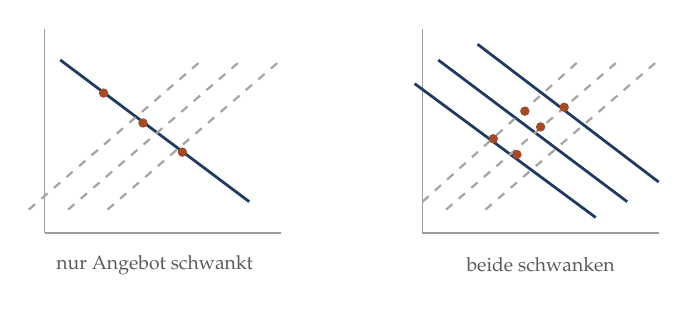
\begin{tikzpicture}[scale=1.0]
\draw[grau!60, line width=0.6pt] (0,0) -- (3.0,0); \draw[grau!60, line width=0.6pt] (0,0) -- (0,2.6);
\draw[tief, line width=1.0pt] (0.2,2.2) -- (2.6,0.4);
\draw[grau!55, line width=0.8pt, dashed] (0.3,0.3) -- (2.5,2.2);
\draw[grau!55, line width=0.8pt, dashed] (0.8,0.3) -- (3.0,2.2);
\draw[grau!55, line width=0.8pt, dashed] (-0.2,0.3) -- (2.0,2.2);
\foreach \x/\y in {0.75/1.78, 1.25/1.4, 1.75/1.03} \fill[akzent] (\x,\y) circle (1.7pt);
\node[font=\scriptsize, color=grau] at (1.4,-0.4) {nur Angebot schwankt};

\draw[grau!60, line width=0.6pt] (4.8,0) -- (7.8,0); \draw[grau!60, line width=0.6pt] (4.8,0) -- (4.8,2.6);
\draw[tief, line width=1.0pt] (5.0,2.2) -- (7.4,0.4);
\draw[tief, line width=1.0pt] (5.5,2.4) -- (7.8,0.65);
\draw[tief, line width=1.0pt] (4.7,1.9) -- (7.0,0.2);
\draw[grau!55, line width=0.8pt, dashed] (5.1,0.3) -- (7.3,2.2);
\draw[grau!55, line width=0.8pt, dashed] (5.6,0.3) -- (7.8,2.2);
\draw[grau!55, line width=0.8pt, dashed] (4.8,0.4) -- (6.8,2.2);
\foreach \x/\y in {5.7/1.2, 6.3/1.35, 6.0/1.0, 6.6/1.6, 6.1/1.55} \fill[akzent] (\x,\y) circle (1.7pt);
\node[font=\scriptsize, color=grau] at (6.3,-0.4) {beide schwanken};
\end{tikzpicture}
\end{center}

\begin{center}
\begin{minipage}{0.88\textwidth}
\kursiv{\textbf{Links zeichnen die Gleichgewichtspunkte die Nachfragekurve nach} --- weil nur das Angebot sich verschiebt. Rechts zeichnen sie eine Wolke, die zu keiner der beiden Kurven gehört. \textbf{Das Problem liegt nicht an zu wenigen Daten}, und es verschwindet nicht, wenn man hundert Jahre weiter beobachtet.}
\end{minipage}
\end{center}
\end{merksatz}

\begin{merksatz}
\boxtitel{Satz 2.1 --- was die Regressionsgerade zeigt}
Im System
\[ q = a - b\,p + u \quad(\text{Nachfrage}), \qquad q = c + d\,p + v \quad(\text{Angebot}) \]
mit unabhängigen Störungen strebt der Kleinste-Quadrate-Koeffizient von $q$ auf $p$ gegen
\[ -b\cdot\frac{\sigma_v^{2}}{\sigma_u^{2}+\sigma_v^{2}} \ + \ d\cdot\frac{\sigma_u^{2}}{\sigma_u^{2}+\sigma_v^{2}} . \]

\schritt{Beweis}
\kursiv{Gleichsetzen liefert den Preis:}
\[ p = \frac{a-c+u-v}{b+d} \quad\Longrightarrow\quad \operatorname{Var}(p) = \frac{\sigma_u^{2}+\sigma_v^{2}}{(b+d)^{2}}, \quad \operatorname{Cov}(p,u) = \frac{\sigma_u^{2}}{b+d} . \]

\kursiv{Aus der Nachfragegleichung:}
\[ \operatorname{Cov}(p,q) = -b\operatorname{Var}(p) + \operatorname{Cov}(p,u) \]
\[ \frac{\operatorname{Cov}(p,q)}{\operatorname{Var}(p)} = -b + \frac{\sigma_u^{2}/(b+d)}{(\sigma_u^{2}+\sigma_v^{2})/(b+d)^{2}} = -b + (b+d)\,\frac{\sigma_u^{2}}{\sigma_u^{2}+\sigma_v^{2}} \]
Umgeordnet ergibt das die Behauptung. $\blacksquare$

\begin{center}
\begin{minipage}{0.9\textwidth}
\textbf{Die geschätzte Gerade ist ein gewogenes Mittel der beiden wahren Steigungen --- gewichtet mit den Varianzanteilen der jeweils \kursiv{anderen} Störung.}
\end{minipage}
\end{center}

\schritt{An $400\,000$ Beobachtungen geprüft}
Wahre Werte: Nachfrage $-0{,}8$, Angebot $+0{,}6$.

\begin{center}
{\small
\renewcommand{\arraystretch}{1.48}
\begin{tabular}{@{}P{1.6cm}P{1.6cm}P{2.0cm}P{2.0cm}@{}}
\toprule
$\sigma_u$ & $\sigma_v$ & \textbf{Formel} & \textbf{simuliert}\\
\midrule
$1$ & $1$ & $-0{,}100$ & $-0{,}099$\\
$1$ & $2$ & $-0{,}520$ & $-0{,}520$\\
$2$ & $1$ & $+0{,}320$ & $+0{,}319$\\
$0{,}2$ & $1$ & $-0{,}746$ & $-0{,}746$\\
$1$ & $0{,}2$ & $+0{,}546$ & $+0{,}546$\\
\bottomrule
\end{tabular}}
\end{center}

\begin{center}
\begin{minipage}{0.9\textwidth}
\textbf{Dieselben Daten können jede Steigung zwischen $-0{,}8$ und $+0{,}6$ zeigen --- je nachdem, welche Seite stärker schwankt.}
\end{minipage}
\end{center}

\begin{center}
\begin{minipage}{0.88\textwidth}
\kursiv{\textbf{Die dritte Zeile ist die schlimmste}: Dort erscheint die Nachfragekurve mit positiver Steigung --- als kauften die Leute mehr, wenn es teurer wird. Solche Befunde finden sich in der Literatur regelmäßig und werden dann mit Qualitätssignalen oder Statuskonsum erklärt. Meist sind sie schlicht das Ergebnis von Satz 2.1.}
\end{minipage}
\end{center}
\end{merksatz}

\section{Identifikation}

\begin{definition}
\boxtitelm{Definition 2.2 --- Identifikation}
Ein Parameter heißt \Begriff{identifiziert}, wenn er durch die Verteilung der beobachtbaren Größen eindeutig bestimmt ist --- wenn also keine zwei Parameterwerte dieselbe beobachtbare Verteilung erzeugen.
\end{definition}

\begin{merksatz}
\boxtitel{Was das heißt und was nicht}
\begin{center}
{\small
\renewcommand{\arraystretch}{1.52}
\begin{tabular}{@{}P{2.4cm}P{6.2cm}@{}}
\toprule
\textbf{Nicht} & eine Frage des Stichprobenumfangs.\\
\textbf{Nicht} & eine Frage des Schätzverfahrens.\\
\textbf{Sondern} & eine Eigenschaft des Modells zusammen mit dem, was beobachtet wird.\\
\bottomrule
\end{tabular}}
\end{center}

\begin{center}
\begin{minipage}{0.9\textwidth}
\textbf{Erst wird gefragt, ob die Größe bei unbegrenzt vielen Daten bestimmbar wäre. Dann erst, wie man sie schätzt.}
\end{minipage}
\end{center}

\begin{center}
\begin{minipage}{0.88\textwidth}
\kursiv{\textbf{Diese Reihenfolge ist der eigentliche Beitrag der Ökonometrie} --- und sie fehlt in weiten Teilen der medizinischen Forschung, wo man gleich zur Schätzung übergeht. Band 23 stellte dieselbe Frage mit Graphen: Gibt es eine zulässige Anpassungsmenge? Hier lautet sie: Lässt sich der Parameter aus den Momenten gewinnen?}
\end{minipage}
\end{center}
\end{merksatz}

\begin{merksatz}
\boxtitel{Satz 2.3 --- die Abzählbedingung}
In einem System simultaner Gleichungen ist eine Gleichung nur dann identifiziert, wenn die Zahl der aus ihr \kursiv{ausgeschlossenen} exogenen Größen mindestens so groß ist wie die Zahl der in ihr enthaltenen endogenen Größen abzüglich eins.

\schritt{Am Beispiel}
\begin{center}
{\small
\renewcommand{\arraystretch}{1.5}
\begin{tabular}{@{}P{2.8cm}P{2.4cm}P{2.8cm}@{}}
\toprule
\textbf{Lage} & \textbf{Ausschlüsse} & \textbf{Nachfrage}\\
\midrule
keine exogene Größe & $0$ & \textcolor{akzent}{nicht identifiziert}\\
Kosten im Angebot & $1$ & \textcolor{gruen}{identifiziert}\\
Einkommen in der Nachfrage & $0$ & \textcolor{akzent}{weiterhin nicht}\\
\bottomrule
\end{tabular}}
\end{center}

\begin{center}
\begin{minipage}{0.88\textwidth}
\kursiv{\textbf{Die dritte Zeile ist der häufigste Irrtum}: Eine Größe, die in der \kursiv{eigenen} Gleichung steht, hilft nicht --- sie verschiebt die eigene Kurve und macht die Lage schlimmer. Identifiziert wird eine Gleichung durch das, was in der \kursiv{anderen} steht und in ihr selbst fehlt. \textbf{Das Ausschließen ist die Annahme, nicht das Einschließen.}}
\end{minipage}
\end{center}

\schritt{Und die Rangbedingung}
\begin{center}
\begin{minipage}{0.88\textwidth}
\kursiv{Die Abzählbedingung ist notwendig, nicht hinreichend --- die ausgeschlossenen Größen müssen auch wirklich wirken. Die genaue Fassung verlangt den Rang einer Matrix; wir übergehen sie --- die erste Auslassung dieses Bandes. \textbf{In der Praxis ist der Rangverlust der Normalfall}: Man hat formal ein Instrument, und es ist zu schwach --- Kapitel~3.}
\end{minipage}
\end{center}
\end{merksatz}

\section{Der Bruchfall}

\begin{warnung}
\boxtitelr{Identifiziert heißt nicht glaubwürdig}
\begin{center}
{\small
\renewcommand{\arraystretch}{1.52}
\begin{tabular}{@{}P{2.8cm}P{5.8cm}@{}}
\toprule
\textbf{Ausschluss ist Annahme} & \enquote{Die Kosten wirken nicht auf die Nachfrage} ist eine Behauptung über die Welt, die niemand prüft.\\
\textbf{Mehr Ausschlüsse} & Je größer das System, desto mehr Ausschlüsse braucht es --- und desto unglaubwürdiger wird jeder einzelne.\\
\textbf{Scheinbare Genauigkeit} & Ein identifiziertes System liefert enge Vertrauensintervalle, deren Gültigkeit vollständig an den Ausschlüssen hängt.\\
\bottomrule
\end{tabular}}
\end{center}

\begin{center}
\begin{minipage}{0.88\textwidth}
\kursiv{\textbf{\Person{Christopher Sims} nannte solche Ausschlüsse 1980 \enquote{unglaubwürdig}} und schlug vor, in Zeitreihenmodellen ganz auf sie zu verzichten --- daraus entstand die Vektorautoregression aus Kapitel~12. Die Identifikationsfrage verschwindet dadurch nicht, sie wandert nur an eine andere Stelle: Statt Gleichungen schließt man dann Wirkungsrichtungen in der kurzen Frist aus.}
\end{minipage}
\end{center}
\end{warnung}

\section{Übungsaufgaben}

\begin{aufgabe}
\boxtitel{Aufgabe 2.1 --- Die Gewichte ausrechnen}
Bei welchem Verhältnis der Störungsvarianzen zeigt die Regression genau null?

\loesung
\schritt{Schritt 1 --- Die Bedingung}
\[ -b\,\frac{\sigma_v^{2}}{\sigma_u^{2}+\sigma_v^{2}} + d\,\frac{\sigma_u^{2}}{\sigma_u^{2}+\sigma_v^{2}} = 0 \quad\Longleftrightarrow\quad \frac{\sigma_u^{2}}{\sigma_v^{2}} = \frac{b}{d} \]

\schritt{Schritt 2 --- Im Beispiel}
\[ \frac{\sigma_u^{2}}{\sigma_v^{2}} = \frac{0{,}8}{0{,}6} = 1{,}333 \quad\Longrightarrow\quad \frac{\sigma_u}{\sigma_v} = 1{,}155 \]

\schritt{Schritt 3 --- Die Probe}
\[ -0{,}8\cdot\frac{1}{2{,}333} + 0{,}6\cdot\frac{1{,}333}{2{,}333} = -0{,}343+0{,}343 = 0 \quad \checkmark \]

\begin{center}
\begin{minipage}{0.9\textwidth}
\textbf{Bei fast ausgeglichenen Schwankungen zeigt die Regression gar keinen Zusammenhang --- obwohl beide Kurven deutlich geneigt sind.}
\end{minipage}
\end{center}

\begin{center}
\begin{minipage}{0.88\textwidth}
\kursiv{\textbf{Ein Nullbefund ist in simultanen Systemen also kein Beleg für Wirkungslosigkeit.} Er kann ebenso gut bedeuten, dass sich zwei starke, entgegengesetzte Wirkungen in der Beobachtung aufheben. Dasselbe gilt für die Rückkopplung zwischen Beitragssatz und Gesundheit aus Aufgabe 1.3.}
\end{minipage}
\end{center}
\end{aufgabe}

\begin{aufgabe}
\boxtitel{Aufgabe 2.2 --- Beobachtungsäquivalenz}
Zeigen Sie, dass verschiedene Parametersätze dieselben Preis-Mengen-Daten erzeugen.

\loesung
\schritt{Schritt 1 --- Was beobachtbar ist}
Nur die drei Momente $\operatorname{Var}(p)$, $\operatorname{Var}(q)$ und $\operatorname{Cov}(p,q)$.

\schritt{Schritt 2 --- Was zu bestimmen wäre}
Vier Größen: $b$, $d$, $\sigma_u^{2}$, $\sigma_v^{2}$.

\begin{center}
\begin{minipage}{0.9\textwidth}
\textbf{Drei Gleichungen, vier Unbekannte --- es bleibt eine ganze Schar von Lösungen.}
\end{minipage}
\end{center}

\schritt{Schritt 3 --- Zwei davon}
\begin{center}
{\small
\renewcommand{\arraystretch}{1.48}
\begin{tabular}{@{}P{1.6cm}P{1.6cm}P{1.6cm}P{1.6cm}P{1.8cm}@{}}
\toprule
$b$ & $d$ & $\sigma_u^{2}$ & $\sigma_v^{2}$ & \textbf{KQ}\\
\midrule
$0{,}80$ & $0{,}60$ & $1{,}00$ & $1{,}00$ & $-0{,}100$\\
$1{,}40$ & $0{,}00$ & $1{,}00$ & $1{,}00$ & $-0{,}700$\\
\bottomrule
\end{tabular}}
\end{center}
\kursiv{Die zweite Zeile lässt sich stets so nachjustieren, dass $\operatorname{Var}(p)$ und $\operatorname{Cov}(p,q)$ übereinstimmen --- ein Freiheitsgrad bleibt übrig.}

\schritt{Schritt 4 --- Die Lehre}
\begin{center}
\begin{minipage}{0.88\textwidth}
\kursiv{\textbf{Das ist Satz 1.2 aus Band 23 in ökonometrischer Fassung}: dieselbe beobachtbare Verteilung, verschiedene zugrunde liegende Größen. Dort waren es zwei Graphen, hier zwei Parametersätze. In beiden Fällen entscheidet keine Datenmenge, sondern nur eine Annahme --- und in beiden Fällen besteht der Fortschritt darin, diese Annahme aufzuschreiben.}
\end{minipage}
\end{center}
\end{aufgabe}

\begin{aufgabe}
\boxtitel{Aufgabe 2.3 --- Die Abzählbedingung anwenden}
Ein Modell der Arztbesuche:
\[ \text{Besuche} = \alpha_1 - \beta\,\text{Zuzahlung} + \gamma\,\text{Alter} + u \]
\[ \text{Zuzahlung} = \alpha_2 + \delta\,\text{Besuche} + \eta\,\text{Beitragssatz} + v \]
Welche Gleichung ist identifiziert?

\loesung
\schritt{Schritt 1 --- Zählen}
\begin{center}
{\small
\renewcommand{\arraystretch}{1.48}
\begin{tabular}{@{}P{2.4cm}P{2.6cm}P{2.6cm}@{}}
\toprule
\textbf{Gleichung} & \textbf{endogen darin} & \textbf{ausgeschlossen}\\
\midrule
Besuche & $2$ & Beitragssatz: $1$\\
Zuzahlung & $2$ & Alter: $1$\\
\bottomrule
\end{tabular}}
\end{center}
Beide erfüllen die Bedingung $1 \ge 2-1$.

\begin{center}
\begin{minipage}{0.9\textwidth}
\textbf{Beide Gleichungen sind identifiziert --- jede durch die Größe, die in der anderen steht.}
\end{minipage}
\end{center}

\schritt{Schritt 2 --- Die Annahmen darin}
\begin{center}
{\small
\renewcommand{\arraystretch}{1.5}
\begin{tabular}{@{}P{2.8cm}P{5.8cm}@{}}
\toprule
\textbf{Beitragssatz} & wirkt \kursiv{nicht} unmittelbar auf die Besuche --- nur über die Zuzahlung.\\
\textbf{Alter} & wirkt \kursiv{nicht} unmittelbar auf die Zuzahlung.\\
\bottomrule
\end{tabular}}
\end{center}

\schritt{Schritt 3 --- Die Prüfung}
\begin{center}
\begin{minipage}{0.88\textwidth}
\kursiv{\textbf{Die zweite Annahme ist falsch}, sobald die Kasse altersabhängige Tarife anbietet --- und die erste, sobald ein hoher Beitragssatz die Versicherten zum Sparen zwingt. \textbf{Formale Identifikation und inhaltliche Haltbarkeit sind zwei verschiedene Dinge}, und die Abzählbedingung prüft nur die erste. Sie ist eine Buchführung über Annahmen, kein Beleg für sie.}
\end{minipage}
\end{center}
\end{aufgabe}

\begin{geschichte}
\boxtitelg{Eine Frage von 1927}
\Person{Elmer Working} veröffentlichte den Aufsatz \kursiv{What Do Statistical Demand Curves Show?} im \kursiv{Quarterly Journal of Economics}.

\begin{center}
\begin{minipage}{0.9\textwidth}
\kursiv{Er beantwortete die Titelfrage mit dem Bild aus Abschnitt 2.1 und schloss, man könne eine Nachfragekurve nur dann schätzen, wenn sie stabil bleibe und das Angebot schwanke. \textbf{Sein Bruder \Person{Holbrook Working} wurde ebenfalls ein bedeutender Ökonometriker}; beide arbeiteten an Agrarmärkten, wo sich das Wetter als Angebotsverschieber anbot.}
\end{minipage}
\end{center}

\schritt{Haavelmo}
\begin{center}
\begin{minipage}{0.9\textwidth}
\kursiv{\Person{Trygve Haavelmo} formulierte 1943 das Identifikationsproblem allgemein und zeigte, dass die Kleinste-Quadrate-Schätzung in simultanen Systemen grundsätzlich verzerrt ist --- Satz 2.1. \textbf{Er schrieb seine Hauptarbeit als junger Forscher in den USA, abgeschnitten von Norwegen durch die deutsche Besetzung.} Der Nobelpreis kam 1989, als er längst zurückgezogen in Oslo lebte.}
\end{minipage}
\end{center}

\schritt{Und die Gegenbewegung}
\begin{center}
\begin{minipage}{0.9\textwidth}
\kursiv{\Person{Edward Leamer} schrieb 1983 den Aufsatz \kursiv{Let's Take the Con Out of Econometrics} --- eine Abrechnung mit der Praxis, Ausschlüsse nach Bedarf zu wählen. \textbf{Sein Vorschlag: Man solle zeigen, wie stark das Ergebnis von den Annahmen abhängt}, statt eine Zahl zu berichten. Die Empfindlichkeitsanalyse aus Band 23, Kapitel~7 geht auf dieselbe Forderung zurück.}
\end{minipage}
\end{center}
\end{geschichte}

\begin{forschung}
\boxtitelp{Identifikation heute}
\begin{center}
{\small
\renewcommand{\arraystretch}{1.45}
\begin{tabular}{@{}P{3.2cm}P{5.0cm}@{}}
\toprule
\textbf{Teilweise Identifikation} & Schranken statt Punktschätzungen, wenn Annahmen fehlen.\\
\textbf{Strukturelle Modelle} & Identifikation aus ökonomischer Theorie statt aus Ausschlüssen.\\
\textbf{Automatische Prüfung} & Rechner, die Identifizierbarkeit aus dem Modell ableiten.\\
\bottomrule
\end{tabular}}
\end{center}

\schritt{Zur ersten Zeile}
\begin{center}
\begin{minipage}{0.88\textwidth}
\kursiv{\Person{Charles Manski} entwickelte ab den 1990er Jahren die Lehre von den Schranken: Statt eine unhaltbare Annahme zu treffen, gibt man an, welches Intervall die Daten zulassen. \textbf{Die Intervalle sind oft weit --- und das ist die Aussage}: Sie zeigen, wie viel die Annahme beiträgt und wie wenig die Daten. Manski nennt das Nachdenken über das, was man nicht weiß, und es ist die ehrlichste Antwort auf Leamers Vorwurf.}
\end{minipage}
\end{center}
\end{forschung}

\begin{merksatz}
\boxtitel{Was Sie jetzt können}
\begin{center}
\renewcommand{\arraystretch}{1.5}
\begin{tabular}{@{}P{3.0cm}P{5.6cm}@{}}
\toprule
\textbf{Satz 2.1} & die Gerade ist ein gewogenes Mittel\\
\textbf{Definition 2.2} & Identifikation vor Schätzung\\
\textbf{Satz 2.3} & Ausschlüsse zählen, nicht Einschlüsse\\
\textbf{Nullbefund} & kann Aufhebung zweier Wirkungen sein\\
\textbf{Der Bruchfall} & identifiziert heißt nicht glaubwürdig\\
\bottomrule
\end{tabular}
\end{center}

\begin{center}
\begin{minipage}{0.88\textwidth}
\kursiv{Die Abzählbedingung sagt, dass eine Größe bestimmbar ist. Das nächste Kapitel sagt, wie man sie bestimmt --- und wie schnell das Verfahren versagt, wenn der Ausschluss zwar gilt, die Wirkung aber schwach ist.}
\end{minipage}
\end{center}
\end{merksatz}

\chapter{Eine Veränderung von außen}

\section{Der Gedanke}

\begin{merksatz}
\boxtitel{Was man braucht}
Die Zuzahlung ist endogen. Gesucht ist eine Größe $z$, die sie verschiebt, ohne selbst mit der Gesundheit zusammenzuhängen.

\begin{center}
{\small
\renewcommand{\arraystretch}{1.55}
\begin{tabular}{@{}P{2.8cm}P{5.8cm}@{}}
\toprule
\textbf{Relevanz} & $\operatorname{Cov}(z,x) \ne 0$ --- prüfbar.\\
\textbf{Exogenität} & $\operatorname{Cov}(z,u) = 0$ --- nicht prüfbar.\\
\bottomrule
\end{tabular}}
\end{center}

\begin{center}
\begin{minipage}{0.88\textwidth}
\kursiv{\textbf{Das ist das Instrument aus Band 23, Kapitel~9} --- dort ein Ausweg, wenn keine Anpassung gelingt, hier der Normalfall einer ganzen Disziplin. Der Unterschied liegt in der Herkunft: Die Epidemiologie sucht Instrumente in der Natur, die Ökonometrie findet sie meist in Gesetzen, Stichtagen und Verwaltungsregeln.}
\end{minipage}
\end{center}

\schritt{Im Leitfall}
Eine Reform erhöht die Zuzahlung in einem Teil der Kassen, aus Gründen, die mit dem Gesundheitszustand der Versicherten nichts zu tun haben.
\end{merksatz}

\begin{merksatz}
\boxtitel{Satz 3.1 --- der Instrumentschätzer}
Erfüllt $z$ beide Bedingungen, so gilt im Modell $y = \beta x + u$
\[ \hat\beta_{\text{IV}} = \frac{\operatorname{Cov}(z,y)}{\operatorname{Cov}(z,x)} \ \longrightarrow\ \beta . \]

\schritt{Beweis}
\[ \operatorname{Cov}(z,y) = \operatorname{Cov}(z,\beta x + u) = \beta\operatorname{Cov}(z,x) + \underbrace{\operatorname{Cov}(z,u)}_{=\,0} \]
Division durch $\operatorname{Cov}(z,x) \ne 0$ liefert $\beta$. $\blacksquare$

\begin{center}
\begin{minipage}{0.9\textwidth}
\textbf{Man benutzt nur denjenigen Teil der Schwankung von $x$, der von $z$ stammt --- und der ist nach Annahme unschuldig.}
\end{minipage}
\end{center}
\end{merksatz}

\section{Zweistufige Schätzung}

\begin{merksatz}
\boxtitel{Dasselbe in zwei Regressionen}
\begin{center}
{\small
\renewcommand{\arraystretch}{1.55}
\begin{tabular}{@{}P{2.4cm}P{6.2cm}@{}}
\toprule
\textbf{Erste Stufe} & $x$ auf $z$ (und alle exogenen Größen) regressieren; die angepassten Werte $\hat x$ behalten.\\
\textbf{Zweite Stufe} & $y$ auf $\hat x$ regressieren.\\
\bottomrule
\end{tabular}}
\end{center}

\begin{center}
\begin{minipage}{0.88\textwidth}
\kursiv{\textbf{Der Vorzug gegenüber Satz 3.1: Das Verfahren verträgt mehrere Instrumente und mehrere Regressoren.} Bei einem Instrument und einem Regressor ergibt es genau denselben Wert --- $\hat x$ ist dann eine lineare Funktion von $z$, und die Kovarianzen kürzen sich.}
\end{minipage}
\end{center}

\schritt{Im Leitfall gerechnet}
$200\,000$ Versicherte, die Reform erhöht die Zuzahlung um $7{,}83$ Euro:

\begin{center}
{\small
\renewcommand{\arraystretch}{1.5}
\begin{tabular}{@{}P{3.4cm}P{2.4cm}@{}}
\toprule
\textbf{Verfahren} & \textbf{je Euro}\\
\midrule
kleinste Quadrate & $-0{,}297$\\
zweistufig & $\mathbf{-0{,}100}$\\
Quotient nach Satz 3.1 & $-0{,}100$\\
\midrule
wahrer Wert & $\mathbf{-0{,}100}$\\
\bottomrule
\end{tabular}}
\end{center}

\begin{center}
\begin{minipage}{0.9\textwidth}
\textbf{Eine einzige exogene Veränderung genügt --- die Gesundheit muss gar nicht gemessen werden.}
\end{minipage}
\end{center}

\begin{center}
\begin{minipage}{0.88\textwidth}
\kursiv{\textbf{Das ist der Grund für die Anziehungskraft des Verfahrens.} Es verlangt nichts über die Störgröße --- weder ihre Messung noch ihre Form --- sondern nur, dass eine bestimmte andere Größe mit ihr nichts zu tun hat. Man tauscht eine unprüfbare Annahme gegen eine andere, und die zweite ist oft leichter zu verteidigen.}
\end{minipage}
\end{center}
\end{merksatz}

\section{Der Bruchfall}

\begin{warnung}
\boxtitelr{Schwache Instrumente}
Dieselbe Rechnung mit $2000$ Versicherten und schwächer werdender Reform, je $500$ Wiederholungen:

\begin{center}
{\small
\renewcommand{\arraystretch}{1.48}
\begin{tabular}{@{}P{2.0cm}P{1.4cm}P{1.8cm}P{3.0cm}@{}}
\toprule
\textbf{Wirkung} & $F$ & \textbf{Median} & \textbf{$5$--$95$ Prozent}\\
\midrule
stark & $719$ & $-0{,}098$ & $[-0{,}121;\ -0{,}073]$\\
mäßig & $44$ & $-0{,}100$ & $[-0{,}177;\ +0{,}019]$\\
schwach & $2{,}8$ & $-0{,}135$ & $\mathbf{[-0{,}805;\ +0{,}922]}$\\
\bottomrule
\end{tabular}}
\end{center}
\kursiv{Zum Vergleich: Die kleinsten Quadrate liefern stets etwa $-0{,}30$.}

\begin{center}
\begin{minipage}{0.9\textwidth}
\textbf{Bei schwachem Instrument reicht das Streuungsband von $-0{,}8$ bis $+0{,}9$ --- die Schätzung ist unbrauchbar, ohne dass es ihr anzusehen wäre.}
\end{minipage}
\end{center}

\schritt{Die beiden Gefahren}
\begin{center}
{\small
\renewcommand{\arraystretch}{1.52}
\begin{tabular}{@{}P{2.6cm}P{6.0cm}@{}}
\toprule
\textbf{Streuung} & Der Nenner ist klein und selbst zufällig --- der Quotient schwankt wild.\\
\textbf{Verzerrung} & Bei schwachem Instrument wandert die Schätzung zum Wert der kleinsten Quadrate hin --- genau dorthin, wovon man wegwollte.\\
\bottomrule
\end{tabular}}
\end{center}

\begin{center}
\begin{minipage}{0.88\textwidth}
\kursiv{\textbf{Die Faustregel $F > 10$ stammt aus einer Arbeit von 1997 und gilt heute als zu großzügig}; neuere Untersuchungen verlangen je nach Lage Werte über hundert. Entscheidend ist, dass $F$ \kursiv{vor} der Schätzung berichtet wird --- und dass ein kleines $F$ nicht zu mehr Instrumenten verleitet, denn jedes schwache zusätzliche verschlimmert die Verzerrung.}
\end{minipage}
\end{center}
\end{warnung}

\begin{warnung}
\boxtitelr{Und die Bedingung, die niemand prüft}
\begin{center}
\begin{minipage}{0.88\textwidth}
\kursiv{Die Exogenität des Instruments ist nicht prüfbar --- außer man hat mehr Instrumente als nötig. \textbf{Dann vergleicht man die Schätzungen}: Weichen sie stärker voneinander ab, als der Zufall erlaubt, so ist mindestens eines ungültig. Das ist der Überidentifikationstest, und er sagt nicht, welches.}
\end{minipage}
\end{center}

\schritt{Gerechnet}
Zwei Instrumente, von denen das zweite unerlaubt unmittelbar auf die Besuche wirkt:

\begin{center}
{\small
\renewcommand{\arraystretch}{1.48}
\begin{tabular}{@{}P{2.6cm}P{2.4cm}P{2.4cm}@{}}
\toprule
\textbf{Instrument} & \textbf{Schätzung} & \\
\midrule
$z_1$ (gültig) & $-0{,}098$ & \textcolor{gruen}{richtig}\\
$z_2$ (ungültig) & $-0{,}013$ & \textcolor{akzent}{falsch}\\
\midrule
Differenz & $\mathbf{0{,}085}$ & Warnsignal\\
\bottomrule
\end{tabular}}
\end{center}

\begin{center}
\begin{minipage}{0.88\textwidth}
\kursiv{\textbf{Besteht man den Test, so ist nichts bewiesen} --- alle Instrumente können gemeinsam in dieselbe Richtung verletzt sein, und dann stimmen die Schätzungen überein, ohne richtig zu sein. Der Test ist eine notwendige Bedingung, wie der Balancetest aus Band 23, Kapitel~7 und der Dichtetest aus Kapitel~10 desselben Bandes.}
\end{minipage}
\end{center}
\end{warnung}

\section{Übungsaufgaben}

\begin{aufgabe}
\boxtitel{Aufgabe 3.1 --- Den Schätzer von Hand}
Aus einer Reform: In Kassen ohne Reform zahlen die Versicherten im Mittel $10{,}4$ Euro und gehen $6{,}95$-mal zum Arzt; in Kassen mit Reform $18{,}2$ Euro und $6{,}17$-mal.

\loesung
\schritt{Schritt 1 --- Die beiden Differenzen}
\[ \Delta x = 18{,}2 - 10{,}4 = 7{,}8 \ \text{Euro}, \qquad \Delta y = 6{,}17 - 6{,}95 = -0{,}78 \ \text{Besuche} \]

\schritt{Schritt 2 --- Der Quotient}
\[ \hat\beta = \frac{-0{,}78}{7{,}8} = \mathbf{-0{,}100} \]

\schritt{Schritt 3 --- Die Deutung der beiden Teile}
\begin{center}
{\small
\renewcommand{\arraystretch}{1.5}
\begin{tabular}{@{}P{2.6cm}P{6.0cm}@{}}
\toprule
\textbf{Zähler} & Wirkung der Reform auf die Besuche --- die Absicht, wie in Band 23, Kapitel~3.\\
\textbf{Nenner} & Wirkung der Reform auf die Zuzahlung --- der Befolgungsgrad.\\
\bottomrule
\end{tabular}}
\end{center}

\begin{center}
\begin{minipage}{0.88\textwidth}
\kursiv{\textbf{Der Schätzer ist die Wirkung der Anordnung, geteilt durch ihre Durchsetzung} --- derselbe Ausdruck wie der Wald-Schätzer aus Band 23. Dort hieß der Nenner Befolgeranteil, hier erste Stufe; die Rechnung ist dieselbe.}
\end{minipage}
\end{center}

\schritt{Schritt 4 --- Die Zielgruppe}
\begin{center}
\begin{minipage}{0.88\textwidth}
\kursiv{Wie dort gilt das Ergebnis für die, deren Zuzahlung sich durch die Reform geändert hat. \textbf{Wer ohnehin einen Hochzuzahlungstarif hatte, trägt nichts bei} --- und wenn solche Versicherten anders reagieren, gilt die Zahl für sie nicht.}
\end{minipage}
\end{center}
\end{aufgabe}

\begin{aufgabe}
\boxtitel{Aufgabe 3.2 --- Warum die zweite Stufe falsche Standardfehler liefert}
Wer die zweite Stufe als gewöhnliche Regression rechnet, erhält zu kleine Streuungen. Warum?

\loesung
\schritt{Schritt 1 --- Der Fehler}
Die gewöhnliche Regression auf $\hat x$ benutzt die Residuen $y - \hat\beta\hat x$. Richtig wären die Residuen $y - \hat\beta x$ --- mit dem \kursiv{tatsächlichen} $x$.

\schritt{Schritt 2 --- Der Unterschied}
\begin{center}
{\small
\renewcommand{\arraystretch}{1.5}
\begin{tabular}{@{}P{2.8cm}P{5.8cm}@{}}
\toprule
\textbf{Falsch} & Die Streuung des Modells wird an den geglätteten Werten gemessen und erscheint kleiner.\\
\textbf{Richtig} & Jedes Programm für zweistufige Schätzung rechnet das automatisch.\\
\bottomrule
\end{tabular}}
\end{center}

\begin{center}
\begin{minipage}{0.9\textwidth}
\textbf{Die beiden Stufen von Hand zu rechnen, liefert den richtigen Koeffizienten und einen falschen Standardfehler.}
\end{minipage}
\end{center}

\schritt{Schritt 3 --- Und die Größenordnung}
\begin{center}
\begin{minipage}{0.88\textwidth}
\kursiv{Der Fehler fällt umso stärker aus, je weniger von $x$ das Instrument erklärt --- also gerade bei schwachen Instrumenten, wo die Streuung ohnehin das Problem ist. \textbf{Beide Fehler wirken in dieselbe Richtung: Man unterschätzt die Unsicherheit dort am meisten, wo sie am größten ist.}}
\end{minipage}
\end{center}
\end{aufgabe}

\begin{aufgabe}
\boxtitel{Aufgabe 3.3 --- Instrumente beurteilen}
Welche der folgenden Größen taugt als Instrument für die Zuzahlung?
\begin{center}
{\small
\renewcommand{\arraystretch}{1.5}
\begin{tabular}{@{}P{1.0cm}P{7.4cm}@{}}
\toprule
(a) & Der Beitragssatz der Kasse.\\
(b) & Das Bundesland, in dem der Versicherte wohnt.\\
(c) & Ein Stichtag: Wer nach dem 1.\ Januar eintritt, erhält den neuen Tarif.\\
\bottomrule
\end{tabular}}
\end{center}

\loesung
\schritt{(a) Beitragssatz}
\begin{center}
{\small
\renewcommand{\arraystretch}{1.48}
\begin{tabular}{@{}P{2.4cm}P{5.8cm}@{}}
\toprule
Relevanz & gegeben\\
Exogenität & \textcolor{akzent}{verletzt} --- der Beitragssatz hängt von der Krankheitslast der Versicherten ab\\
\bottomrule
\end{tabular}}
\end{center}

\schritt{(b) Bundesland}
\begin{center}
{\small
\renewcommand{\arraystretch}{1.48}
\begin{tabular}{@{}P{2.4cm}P{5.8cm}@{}}
\toprule
Relevanz & gegeben, wenn die Tarife regional verschieden sind\\
Exogenität & \textcolor{akzent}{zweifelhaft} --- Bundesländer unterscheiden sich in Alter, Einkommen und Arztdichte\\
\bottomrule
\end{tabular}}
\end{center}

\schritt{(c) Stichtag}
\begin{center}
{\small
\renewcommand{\arraystretch}{1.48}
\begin{tabular}{@{}P{2.4cm}P{5.8cm}@{}}
\toprule
Relevanz & gegeben\\
Exogenität & \textcolor{gruen}{haltbar} --- wer am 28.\ Dezember eintritt, unterscheidet sich kaum von dem, der am 3.\ Januar eintritt\\
\bottomrule
\end{tabular}}
\end{center}

\begin{center}
\begin{minipage}{0.9\textwidth}
\textbf{Nur der Stichtag taugt --- und auch er nur in einem schmalen Fenster um den Termin.}
\end{minipage}
\end{center}

\schritt{Die Prüfung}
\begin{center}
\begin{minipage}{0.88\textwidth}
\kursiv{\textbf{Man prüft einen Stichtag wie eine Schwelle in Band 23, Kapitel~10}: Häufen sich die Eintritte unmittelbar vor dem Termin, so haben die Versicherten die Regel verstanden und sich sortiert --- dann ist die Exogenität dahin. \textbf{Dieselbe Rechnung, dasselbe Warnsignal, andere Fachsprache.} Die Ökonometrie nennt es Manipulation der Zuweisungsvariablen.}
\end{minipage}
\end{center}
\end{aufgabe}

\begin{geschichte}
\boxtitelg{Ein Anhang über Pflanzenöle}
\Person{Philip Wright} beschrieb den Instrumentschätzer 1928 im Anhang B eines Buches über Zölle auf Pflanzenöle --- Band 23, Kapitel~9 erzählt die Geschichte ausführlicher.

\begin{center}
\begin{minipage}{0.9\textwidth}
\kursiv{\textbf{Bemerkenswert ist, dass das Verfahren danach für Jahrzehnte verschwand}: Die Cowles-Kommission entwickelte in den 1940er Jahren die zweistufige Schätzung unabhängig und als Teil der Theorie simultaner Gleichungen. Erst in den 1990er Jahren wurde sie wieder als eigenständiges Werkzeug begriffen --- nicht als Lösung eines Systems, sondern als Ausnutzung einer einzelnen glaubwürdigen Veränderung.}
\end{minipage}
\end{center}

\schritt{Die Wende}
\begin{center}
\begin{minipage}{0.9\textwidth}
\kursiv{\Person{Joshua Angrist} und \Person{Alan Krueger} benutzten 1991 das Geburtsquartal als Instrument für die Schulbesuchsdauer --- weil die Schulpflicht an Geburtstage anknüpft. \textbf{Der Aufsatz machte Schule und wurde zugleich zum Lehrbeispiel für schwache Instrumente}: \Person{Bound}, \Person{Jaeger} und \Person{Baker} zeigten 1995, dass die Ergebnisse bei zufällig erzeugten Instrumenten fast genauso aussahen.}
\end{minipage}
\end{center}

\schritt{Und der Nobelpreis}
\begin{center}
\begin{minipage}{0.9\textwidth}
\kursiv{2021 erhielten \Person{Angrist} und \Person{Guido Imbens} den Preis für die Klärung, was Instrumente eigentlich schätzen --- den Effekt bei den Befolgern. \textbf{\Person{David Card} erhielt ihn zugleich für die Arbeiten zu natürlichen Versuchen}, und die Begründung nannte ausdrücklich die Verbindung von beidem: glaubwürdige Veränderung plus saubere Deutung dessen, was man misst.}
\end{minipage}
\end{center}
\end{geschichte}

\begin{forschung}
\boxtitelp{Instrumente heute}
\begin{center}
{\small
\renewcommand{\arraystretch}{1.45}
\begin{tabular}{@{}P{3.2cm}P{5.0cm}@{}}
\toprule
\textbf{Schwache Instrumente} & Verfahren, die auch bei kleinem $F$ gültige Intervalle liefern.\\
\textbf{Viele Instrumente} & Auswahl mit Lernverfahren --- und die Verzerrung, die daraus folgt.\\
\textbf{Fast gültig} & Schranken, wenn die Ausschlussbedingung nur ungefähr gilt.\\
\bottomrule
\end{tabular}}
\end{center}

\schritt{Zur ersten Zeile}
\begin{center}
\begin{minipage}{0.88\textwidth}
\kursiv{Es gibt Verfahren, deren Vertrauensintervalle unabhängig von der Instrumentstärke gültig bleiben --- der Anderson-Rubin-Test ist das bekannteste. \textbf{Bei sehr schwachen Instrumenten liefert er dann allerdings die ganze reelle Achse}, und genau das ist die richtige Antwort: Die Daten sagen nichts. Dass dieses Ergebnis selten berichtet wird, liegt nicht an der Methodik.}
\end{minipage}
\end{center}
\end{forschung}

\begin{merksatz}
\boxtitel{Was Sie jetzt können}
\begin{center}
\renewcommand{\arraystretch}{1.5}
\begin{tabular}{@{}P{3.0cm}P{5.6cm}@{}}
\toprule
\textbf{Satz 3.1} & $\operatorname{Cov}(z,y)/\operatorname{Cov}(z,x)$\\
\textbf{Zweistufig} & verträgt mehrere Instrumente\\
\textbf{Schwach} & Streuung und Verzerrung zugleich\\
\textbf{Überidentifiz.} & notwendige Bedingung, kein Beweis\\
\textbf{Stichtage} & die glaubwürdigsten Instrumente\\
\bottomrule
\end{tabular}
\end{center}

\begin{center}
\begin{minipage}{0.88\textwidth}
\kursiv{Damit endet Teil~I. Der Instrumentschätzer ist ein Sonderfall eines allgemeineren Gedankens: Man schreibt auf, welche Momente null sein müssen, und sucht die Parameter, die das erfüllen. Teil~II beginnt mit dieser Verallgemeinerung.}
\end{minipage}
\end{center}
\end{merksatz}

\part{Querschnittsdaten}

\chapter{Momente statt Verteilungen}

\section{Der gemeinsame Nenner}

\begin{merksatz}
\boxtitel{Drei Schätzer, ein Prinzip}
\begin{center}
{\small
\renewcommand{\arraystretch}{1.55}
\begin{tabular}{@{}P{2.8cm}P{5.8cm}@{}}
\toprule
\textbf{Kleinste Quadrate} & $\mathbb{E}[x\,(y-\beta x)] = 0$\\
\textbf{Instrument} & $\mathbb{E}[z\,(y-\beta x)] = 0$\\
\textbf{Mittelwert} & $\mathbb{E}[y - \mu] = 0$\\
\bottomrule
\end{tabular}}
\end{center}

\begin{center}
\begin{minipage}{0.9\textwidth}
\textbf{Jeder dieser Schätzer ist die Lösung einer Gleichung, die sagt: Ein bestimmter Erwartungswert ist null.}
\end{minipage}
\end{center}

\begin{center}
\begin{minipage}{0.88\textwidth}
\kursiv{\textbf{Die Maximum-Likelihood-Schätzung aus Band 17 verlangt die ganze Verteilung}; hier verlangt man nur, dass bestimmte Mittelwerte stimmen. Das ist weniger --- und deshalb robuster. Ökonomische Theorie liefert fast nie Verteilungen, aber oft Bedingungen der Form \enquote{im Mittel gleicht sich das aus}: Gleichgewicht, Erwartungstreue, Fairness. Jede solche Bedingung ist ein Moment.}
\end{minipage}
\end{center}
\end{merksatz}

\begin{definition}
\boxtitelm{Definition 4.1 --- Momentenbedingung und Momentenschätzer}
Eine \Begriff{Momentenbedingung} ist eine Gleichung
\[ \mathbb{E}\bigl[g(w,\theta)\bigr] = 0 , \]
in der $w$ die beobachteten Größen und $\theta$ den Parameter bezeichnet. Der \Begriff{Momentenschätzer} ersetzt den Erwartungswert durch das Stichprobenmittel und löst
\[ \frac1n\sum_{i=1}^{n} g(w_i,\hat\theta) = 0 . \]
\end{definition}

\begin{merksatz}
\boxtitel{Satz 4.2 --- Konsistenz}
Gilt die Momentenbedingung, ist $\theta$ dadurch eindeutig bestimmt und ist $g$ stetig, so strebt $\hat\theta$ gegen $\theta$.

\schritt{Der Gedanke}
Nach dem Gesetz der großen Zahlen strebt das Stichprobenmittel gegen den Erwartungswert --- für jedes feste $\theta$. Die Lösung einer Gleichung, deren linke Seite gleichmäßig gegen eine Grenzfunktion strebt, strebt gegen die Lösung der Grenzgleichung, sofern diese eindeutig ist. $\blacksquare$

\begin{center}
\begin{minipage}{0.88\textwidth}
\kursiv{\textbf{Die Eindeutigkeit ist die Identifikation aus Kapitel~2} --- hier in der Form: Die Momentenbedingung hat genau eine Lösung. Die Gleichmäßigkeit der Konvergenz ist technisch und wird meist stillschweigend vorausgesetzt; wir übergehen ihren Nachweis --- die zweite Auslassung dieses Bandes.}
\end{minipage}
\end{center}
\end{merksatz}

\section{Mehr Bedingungen als Parameter}

\begin{merksatz}
\boxtitel{Das Problem}
Mit zwei Instrumenten $z_1$, $z_2$ und einem Parameter $\beta$ hat man zwei Gleichungen für eine Unbekannte:
\[ \frac1n\sum z_{1i}(y_i-\beta x_i) = 0, \qquad \frac1n\sum z_{2i}(y_i-\beta x_i) = 0 . \]

\begin{center}
\begin{minipage}{0.9\textwidth}
\textbf{In der Stichprobe lassen sich beide nie gleichzeitig exakt erfüllen. Man muss einen Kompromiss wählen.}
\end{minipage}
\end{center}
\end{merksatz}

\begin{definition}
\boxtitelm{Definition 4.3 --- verallgemeinerte Momentenmethode}
Sei $\bar g(\theta) = \frac1n\sum g(w_i,\theta)$ der Vektor der Stichprobenmomente und $W$ eine positiv definite Gewichtsmatrix. Der \Begriff{GMM-Schätzer} minimiert
\[ Q(\theta) = \bar g(\theta)^{\top}\,W\,\bar g(\theta) . \]
\end{definition}

\begin{merksatz}
\boxtitel{Satz 4.4 --- die beste Gewichtung}
Unter allen Gewichtsmatrizen liefert
\[ W^{*} = S^{-1}, \qquad S = \operatorname{Var}\bigl[g(w,\theta)\bigr] \]
den Schätzer mit kleinster Varianz.

\schritt{Der Gedanke}
Momente, die stark streuen, sind weniger verlässlich und sollen weniger zählen; Momente, die miteinander korrelieren, tragen gemeinsam weniger bei, als ihre Zahl vermuten lässt. Beides leistet die inverse Varianzmatrix --- derselbe Gedanke wie bei den gewichteten kleinsten Quadraten in Band 17, Kapitel~8. $\blacksquare$

\begin{center}
\begin{minipage}{0.88\textwidth}
\kursiv{\textbf{In der Praxis rechnet man zweimal}: erst mit einer beliebigen Gewichtung, um $\theta$ grob zu schätzen und daraus $S$ zu bestimmen, dann mit $S^{-1}$. Die zweistufige Schätzung aus Kapitel~3 ist der Sonderfall $W = (Z^{\top}Z)^{-1}$ --- optimal nur, wenn die Störungen gleich streuen.}
\end{minipage}
\end{center}

\schritt{Im Leitfall}
Zwei Instrumente für die Zuzahlung --- die Reform und ein regionaler Tarifunterschied:

\begin{center}
{\small
\renewcommand{\arraystretch}{1.48}
\begin{tabular}{@{}P{3.4cm}P{2.4cm}@{}}
\toprule
\textbf{Verfahren} & \textbf{je Euro}\\
\midrule
nur Reform & $-0{,}0980$\\
nur Region & $-0{,}0987$\\
zweistufig, beide & $-0{,}0982$\\
GMM, effizient & $\mathbf{-0{,}0982}$\\
\bottomrule
\end{tabular}}
\end{center}
\kursiv{Bei gleichmäßig streuenden Störungen fallen zweistufige und effiziente Schätzung zusammen --- wie der Satz es verlangt.}
\end{merksatz}

\section{Die überschüssigen Bedingungen prüfen}

\begin{merksatz}
\boxtitel{Satz 4.5 --- der Test von Hansen}
Gelten alle Momentenbedingungen, so ist
\[ J = n\,\bar g(\hat\theta)^{\top}\,\hat S^{-1}\,\bar g(\hat\theta) \]
asymptotisch $\chi^{2}$-verteilt mit so vielen Freiheitsgraden, wie es Bedingungen mehr als Parameter gibt.

\schritt{Der Gedanke}
Mit $m$ Bedingungen und $k$ Parametern kann man $k$ Bedingungen exakt erfüllen. Die übrigen $m-k$ müssen \kursiv{von selbst} nahe null sein --- und wie nahe, sagt ihre Streuung. $J$ misst den gewichteten Abstand der überschüssigen Momente von null. $\blacksquare$

\schritt{Im Leitfall}
\begin{center}
{\small
\renewcommand{\arraystretch}{1.48}
\begin{tabular}{@{}P{3.2cm}P{2.0cm}P{2.4cm}@{}}
\toprule
\textbf{Lage} & $J$ & \textbf{Urteil}\\
\midrule
beide gültig & $0{,}09$ & \textcolor{gruen}{unauffällig}\\
Region wirkt direkt & $\mathbf{1782}$ & \textcolor{akzent}{verworfen}\\
\bottomrule
\end{tabular}}
\end{center}
\kursiv{Grenze bei einem Freiheitsgrad: $3{,}84$.}

\begin{center}
\begin{minipage}{0.9\textwidth}
\textbf{Der Test ist der Überidentifikationstest aus Kapitel~3, nun als allgemeines Prinzip --- und er sagt weiterhin nicht, welche Bedingung verletzt ist.}
\end{minipage}
\end{center}
\end{merksatz}

\section{Der Bruchfall}

\begin{warnung}
\boxtitelr{Zu viele Momente}
\begin{center}
{\small
\renewcommand{\arraystretch}{1.52}
\begin{tabular}{@{}P{2.8cm}P{5.8cm}@{}}
\toprule
\textbf{Die Verlockung} & Jede Funktion eines gültigen Instruments ist wieder ein gültiges Instrument: $z$, $z^{2}$, $z^{3}$, $z\cdot x_2$ \ldots\\
\textbf{Die Folge} & Mit vielen Momenten wird $\hat S$ schlecht geschätzt, die Gewichtung unsinnig und der Schätzer verzerrt --- in Richtung der kleinsten Quadrate.\\
\textbf{Die Regel} & Die Zahl der Momente soll gegenüber $n$ klein bleiben; der Test aus Satz 4.5 verliert bei vielen Momenten seine Aussagekraft.\\
\bottomrule
\end{tabular}}
\end{center}

\begin{center}
\begin{minipage}{0.88\textwidth}
\kursiv{\textbf{Das ist das Problem der schwachen Instrumente aus Kapitel~3 in anderer Gestalt}: Viele Instrumente, von denen jedes wenig erklärt, wirken wie ein einziges schwaches. Die Literatur über Panelmodelle in Kapitel~8 kennt den Fall besonders gut, weil dort die Instrumente mit jeder Zeitperiode von selbst mehr werden.}
\end{minipage}
\end{center}
\end{warnung}

\begin{warnung}
\boxtitelr{Und was Momente nicht liefern}
\begin{center}
\begin{minipage}{0.88\textwidth}
\kursiv{Die Momentenmethode schätzt Parameter, keine Verteilungen. \textbf{Wer wissen will, wie viele Versicherte \kursiv{gar nicht} mehr zum Arzt gehen}, braucht die Verteilung der Besuchszahlen --- und die liefert nur ein vollständiges Modell. Das nächste Kapitel gibt eines an, und bezahlt dafür mit einer Verteilungsannahme.}
\end{minipage}
\end{center}
\end{warnung}

\section{Übungsaufgaben}

\begin{aufgabe}
\boxtitel{Aufgabe 4.1 --- Momentenschätzer von Hand}
Die Zahl der Arztbesuche sei poissonverteilt. Leiten Sie den Momentenschätzer für $\lambda$ aus zwei verschiedenen Momenten her.

\loesung
\schritt{Schritt 1 --- Erstes Moment}
\[ \mathbb{E}[y - \lambda] = 0 \quad\Longrightarrow\quad \hat\lambda_1 = \bar y \]

\schritt{Schritt 2 --- Zweites Moment}
Bei Poisson gilt $\operatorname{Var}[y] = \lambda$:
\[ \mathbb{E}\bigl[(y-\lambda)^{2} - \lambda\bigr] = 0 \quad\Longrightarrow\quad \hat\lambda_2 = \text{Stichprobenvarianz} \]

\schritt{Schritt 3 --- Die Zahlen}
$5000$ simulierte Versicherte mit $\lambda = 3{,}2$:
\begin{center}
{\small
\renewcommand{\arraystretch}{1.48}
\begin{tabular}{@{}P{2.6cm}P{2.4cm}@{}}
\toprule
\textbf{Moment} & $\hat\lambda$\\
\midrule
Mittelwert & $3{,}234$\\
Varianz & $3{,}290$\\
\bottomrule
\end{tabular}}
\end{center}

\schritt{Schritt 4 --- Die Deutung}
\begin{center}
\begin{minipage}{0.9\textwidth}
\textbf{Zwei Momente, ein Parameter --- die Lage von Satz 4.4. Der Mittelwert ist der bessere Schätzer, und GMM gewichtet ihn entsprechend stärker.}
\end{minipage}
\end{center}

\begin{center}
\begin{minipage}{0.88\textwidth}
\kursiv{\textbf{Der Unterschied der beiden Schätzungen ist zugleich ein Test}: Weichen Mittelwert und Varianz deutlich voneinander ab, so ist die Zahl nicht poissonverteilt --- das ist die Prüfgröße aus Band 25, Aufgabe 4.3, nun als Spezialfall von Satz 4.5. Bei Arztbesuchen fällt der Test regelmäßig durch: Die Varianz übersteigt den Mittelwert um ein Mehrfaches.}
\end{minipage}
\end{center}
\end{aufgabe}

\begin{aufgabe}
\boxtitel{Aufgabe 4.2 --- Die Gewichtsmatrix verstehen}
Zwei Momente mit Varianzen $1$ und $4$, unkorreliert. Wie gewichtet GMM?

\loesung
\schritt{Schritt 1 --- Die Matrix}
\[ S = \begin{pmatrix} 1 & 0\\ 0 & 4\end{pmatrix}, \qquad W^{*} = S^{-1} = \begin{pmatrix} 1 & 0\\ 0 & \tfrac14\end{pmatrix} \]

\schritt{Schritt 2 --- Das Kriterium}
\[ Q(\theta) = \bar g_1^{2} + \tfrac14\,\bar g_2^{2} \]

\begin{center}
\begin{minipage}{0.9\textwidth}
\textbf{Das streuende Moment zählt nur ein Viertel --- im Verhältnis der inversen Varianzen.}
\end{minipage}
\end{center}

\schritt{Schritt 3 --- Mit Korrelation}
Sind die Momente mit $\rho = 0{,}9$ korreliert, so wird
\[ S^{-1} = \frac{1}{4(1-0{,}81)}\begin{pmatrix} 4 & -1{,}8\\ -1{,}8 & 1\end{pmatrix} = \begin{pmatrix} 5{,}26 & -2{,}37\\ -2{,}37 & 1{,}32\end{pmatrix} \]

\begin{center}
\begin{minipage}{0.88\textwidth}
\kursiv{\textbf{Die Nebendiagonale ist negativ}: Zwei fast gleichlautende Bedingungen werden nicht doppelt, sondern nach ihrem \kursiv{Unterschied} gewichtet. Das ist der Grund, warum das Hinzufügen fast gleicher Instrumente nichts bringt --- und warum die Gewichtsmatrix bei vielen Momenten kaum schätzbar ist: Sie muss die Korrelationen aller Paare kennen.}
\end{minipage}
\end{center}
\end{aufgabe}

\begin{aufgabe}
\boxtitel{Aufgabe 4.3 --- Ein Modell mit Erwartungen}
Ein Haushalt plant seinen Konsum so, dass $\mathbb{E}_t[u'(c_{t+1})\,R_{t+1}] = \delta\,u'(c_t)$ gilt --- die Eulergleichung der Konsumtheorie. Wie schätzt man $\delta$ ohne Verteilungsannahme?

\loesung
\schritt{Schritt 1 --- Die Momentenbedingung}
\[ \mathbb{E}_t\left[\frac{u'(c_{t+1})}{u'(c_t)}\,R_{t+1} - \frac1\delta\right] = 0 \]
--- bedingt auf alles, was zur Zeit $t$ bekannt ist.

\schritt{Schritt 2 --- Instrumente}
Jede zur Zeit $t$ bekannte Größe $z_t$ darf mit dem Ausdruck multipliziert werden; nach der Turmregel aus Band 25, Satz 7.3, bleibt der unbedingte Erwartungswert null:
\[ \mathbb{E}\left[z_t\left(\frac{u'(c_{t+1})}{u'(c_t)}R_{t+1} - \frac1\delta\right)\right] = 0 \]

\schritt{Schritt 3 --- Was das leistet}
\begin{center}
\begin{minipage}{0.9\textwidth}
\textbf{Man schätzt einen Parameter des Verhaltens, ohne anzugeben, wie Einkommen, Zinsen oder Preise verteilt sind.}
\end{minipage}
\end{center}

\begin{center}
\begin{minipage}{0.88\textwidth}
\kursiv{\textbf{Das ist die Anwendung, für die GMM 1982 entwickelt wurde} --- \Person{Hansen} und \Person{Singleton} schätzten damit die Risikoscheu amerikanischer Haushalte. Das Ergebnis war ernüchternd: Die Bedingungen wurden verworfen, und zwar deutlich. Die Differenz zwischen beobachteten Aktienrenditen und dem, was die Eulergleichung erlaubt, heißt seither Aktienprämienrätsel und ist nicht gelöst.}
\end{minipage}
\end{center}

\schritt{Schritt 4 --- Die Verbindung}
\begin{center}
\begin{minipage}{0.88\textwidth}
\kursiv{Die Momentenbedingung ist eine Martingalbedingung: Der Ausdruck in der Klammer ist eine Martingaldifferenz. \textbf{Band 25 lieferte den Begriff, dieses Kapitel benutzt ihn als Schätzgleichung}, und Kapitel~11 wird ihn zur Prüfung der Markteffizienz heranziehen.}
\end{minipage}
\end{center}
\end{aufgabe}

\begin{geschichte}
\boxtitelg{Von Pearson zu Hansen}
\Person{Karl Pearson} führte die Momentenmethode 1894 ein --- um eine Mischung zweier Normalverteilungen an Krabbenmessungen anzupassen, die sein Kollege \Person{Weldon} aus Neapel mitgebracht hatte.

\begin{center}
\begin{minipage}{0.9\textwidth}
\kursiv{Er setzte die ersten fünf theoretischen Momente den empirischen gleich und löste ein Polynom neunten Grades. \textbf{\Person{Fisher} verdrängte das Verfahren ab 1922 mit der Maximum-Likelihood-Methode}, die bei bekannter Verteilung effizienter ist --- und die Momentenmethode galt sechzig Jahre lang als überholt.}
\end{minipage}
\end{center}

\schritt{Die Wiederkehr}
\begin{center}
\begin{minipage}{0.9\textwidth}
\kursiv{\Person{Lars Peter Hansen} verallgemeinerte 1982 den Ansatz auf beliebig viele Bedingungen und bewies Satz 4.4 und 4.5. \textbf{Der Anlass war die Konsumtheorie aus Aufgabe 4.3}: Ökonomische Modelle liefern Momentenbedingungen, keine Verteilungen, und Fishers Methode war dafür nicht zu gebrauchen. Hansen erhielt 2013 den Nobelpreis --- gemeinsam mit \Person{Fama} und \Person{Shiller}, deren Streit über Markteffizienz Kapitel~11 aufnimmt.}
\end{minipage}
\end{center}

\schritt{Und die Einordnung}
\begin{center}
\begin{minipage}{0.9\textwidth}
\kursiv{\textbf{Fast alle Schätzer dieses Bandes sind Sonderfälle von GMM} --- kleinste Quadrate, Instrumente, zweistufige Schätzung, und auch Maximum Likelihood, wenn man die Ableitung der Likelihood als Moment auffasst. Die Methode ist weniger ein Verfahren als eine Sprache, in der sich die anderen Verfahren vergleichen lassen.}
\end{minipage}
\end{center}
\end{geschichte}

\begin{forschung}
\boxtitelp{Momentenschätzung heute}
\begin{center}
{\small
\renewcommand{\arraystretch}{1.45}
\begin{tabular}{@{}P{3.2cm}P{5.0cm}@{}}
\toprule
\textbf{Empirische Likelihood} & Gewichte statt Gewichtsmatrix --- bessere Eigenschaften bei kleinen Stichproben.\\
\textbf{Viele Momente} & Regularisierung der Gewichtsmatrix, Auswahl von Instrumenten.\\
\textbf{Orthogonalisierte Momente} & Momente, die gegen Fehler in Hilfsgrößen unempfindlich sind.\\
\bottomrule
\end{tabular}}
\end{center}

\schritt{Zur dritten Zeile}
\begin{center}
\begin{minipage}{0.88\textwidth}
\kursiv{Schätzt man Kontrollgrößen mit Lernverfahren aus Band 22, so überträgt sich deren Fehler auf den Effekt --- außer man wählt die Momentenbedingung so, dass ihre Ableitung nach den Hilfsgrößen null ist. \textbf{Das ist der Kern des \enquote{doppelt robusten} maschinellen Lernens} von \Person{Chernozhukov} und Mitarbeitern aus dem Jahr 2018 --- und derselbe Gedanke wie die doppelte Absicherung aus Band 23, Kapitel~8, nun als Eigenschaft eines Moments formuliert.}
\end{minipage}
\end{center}
\end{forschung}

\begin{merksatz}
\boxtitel{Was Sie jetzt können}
\begin{center}
\renewcommand{\arraystretch}{1.5}
\begin{tabular}{@{}P{3.0cm}P{5.6cm}@{}}
\toprule
\textbf{Definition 4.1} & Schätzer als Nullstelle eines Mittelwerts\\
\textbf{Satz 4.2} & Konsistenz aus dem Gesetz der großen Zahlen\\
\textbf{Satz 4.4} & inverse Varianz gewichtet optimal\\
\textbf{Satz 4.5} & überschüssige Momente prüfen\\
\textbf{Der Bruchfall} & viele Momente wirken wie ein schwaches\\
\bottomrule
\end{tabular}
\end{center}

\begin{center}
\begin{minipage}{0.88\textwidth}
\kursiv{Alle bisherigen Zielgrößen waren stetig und unbeschränkt. Das nächste Kapitel behandelt Entscheidungen --- ja oder nein --- und Größen, die bei null abgeschnitten sind. Dort braucht man wieder eine Verteilung, und man erfährt, was sie kostet.}
\end{minipage}
\end{center}
\end{merksatz}

\chapter{Ja oder nein, null oder mehr}

\section{Eine Entscheidung erklären}

\begin{merksatz}
\boxtitel{Geht jemand zum Facharzt?}
Die Zielgröße ist nun $y \in \{0,1\}$: ob ein Versicherter im Jahr mindestens einmal einen Facharzt aufsucht. Im Leitfall tun das $21$ Prozent.

\begin{center}
\begin{minipage}{0.9\textwidth}
\textbf{Eine Regression auf $y$ schätzt eine Wahrscheinlichkeit --- und Wahrscheinlichkeiten liegen zwischen null und eins. Die Gerade weiß das nicht.}
\end{minipage}
\end{center}
\end{merksatz}

\begin{definition}
\boxtitelm{Definition 5.1 --- Logit und Probit}
Man modelliert die Wahrscheinlichkeit als Funktion eines linearen Index:
\[ \Pr[y = 1 \mid x] = F(x^{\top}\beta), \qquad F(t) = \begin{cases} \dfrac{1}{1+e^{-t}} & \text{Logit}\\[8pt] \Phi(t) & \text{Probit}\end{cases} \]
Geschätzt wird $\beta$ durch Maximum Likelihood:
\[ \ell(\beta) = \sum_i \Bigl[y_i\ln F(x_i^{\top}\beta) + (1-y_i)\ln\bigl(1-F(x_i^{\top}\beta)\bigr)\Bigr] . \]
\end{definition}

\begin{merksatz}
\boxtitel{Die latente Deutung}
Man stelle sich eine unbeobachtete Neigung $y^{*} = x^{\top}\beta + \varepsilon$ vor; beobachtet wird nur, ob sie eine Schwelle überschreitet:
\[ y = \mathbf 1\{y^{*} > 0\} \quad\Longrightarrow\quad \Pr[y=1\mid x] = \Pr[\varepsilon > -x^{\top}\beta] = F(x^{\top}\beta) . \]

\begin{center}
{\small
\renewcommand{\arraystretch}{1.5}
\begin{tabular}{@{}P{2.4cm}P{6.2cm}@{}}
\toprule
\textbf{Probit} & $\varepsilon$ normalverteilt.\\
\textbf{Logit} & $\varepsilon$ logistisch verteilt --- fast dieselbe Form, schwerere Ränder.\\
\bottomrule
\end{tabular}}
\end{center}

\begin{center}
\begin{minipage}{0.88\textwidth}
\kursiv{\textbf{Die latente Neigung ist der Nutzen aus Band 24}: Der Versicherte geht, wenn der Nutzen des Besuchs den der Alternative übersteigt. Damit wird aus einem statistischen Modell ein Entscheidungsmodell --- und $\beta$ erhält eine Deutung als Gewicht im Nutzen. Das ist der Grund, warum die Ökonometrie diese Modelle als \enquote{diskrete Wahl} bezeichnet.}
\end{minipage}
\end{center}
\end{merksatz}

\section{Was ein Koeffizient bedeutet}

\begin{merksatz}
\boxtitel{Satz 5.2 --- der Randeffekt}
Die Änderung der Wahrscheinlichkeit je Einheit von $x_j$ beträgt
\[ \frac{\partial\Pr[y=1\mid x]}{\partial x_j} = \beta_j\,f(x^{\top}\beta) \]
mit der Dichte $f = F'$. Beim Logit ist $f(t) = F(t)\bigl(1-F(t)\bigr)$.

\schritt{Beweis}
Kettenregel. $\blacksquare$

\begin{center}
\begin{minipage}{0.9\textwidth}
\textbf{Der Koeffizient ist keine Wirkung. Die Wirkung hängt davon ab, wo man steht --- und sie ist am größten bei fünfzig Prozent.}
\end{minipage}
\end{center}

\schritt{Im Leitfall}
Logit mit Alter und Zuzahlung, $100\,000$ Versicherte:

\begin{center}
{\small
\renewcommand{\arraystretch}{1.48}
\begin{tabular}{@{}P{3.6cm}P{2.6cm}@{}}
\toprule
\textbf{Größe} & \textbf{je Euro Zuzahlung}\\
\midrule
Koeffizient $\beta$ & $-0{,}0374$\\
Randeffekt bei $p = 0{,}5$ & $-0{,}0093$\\
mittlerer Randeffekt & $\mathbf{-0{,}0059}$\\
lineares Modell & $-0{,}0059$\\
\bottomrule
\end{tabular}}
\end{center}

\begin{center}
\begin{minipage}{0.88\textwidth}
\kursiv{\textbf{Der Randeffekt am Mittel und der mittlere Randeffekt unterscheiden sich um die Hälfte} --- weil die meisten Versicherten weit unter fünfzig Prozent liegen, wo die Kurve flach ist. Und das lineare Wahrscheinlichkeitsmodell trifft den mittleren Randeffekt genau: \textbf{Für die mittlere Wirkung braucht man das Logit nicht.} Man braucht es für Vorhersagen am Rand, für Untergruppen und für die Nutzendeutung.}
\end{minipage}
\end{center}
\end{merksatz}

\section{Null oder mehr}

\begin{merksatz}
\boxtitel{Ausgaben mit Nullen}
Nun seien die Arztkosten eines Jahres die Zielgröße. Bei $32$ Prozent der Versicherten sind sie null.

\begin{center}
{\small
\renewcommand{\arraystretch}{1.48}
\begin{tabular}{@{}P{3.4cm}P{2.4cm}@{}}
\toprule
\textbf{Verfahren} & \textbf{je Euro}\\
\midrule
KQ, alle Versicherten & $-1{,}38$\\
KQ, nur Zahler & $-1{,}00$\\
\midrule
wahre Steigung der Neigung & $\mathbf{-2{,}00}$\\
\bottomrule
\end{tabular}}
\end{center}

\begin{center}
\begin{minipage}{0.9\textwidth}
\textbf{Beide Regressionen unterschätzen --- und das Weglassen der Nullen macht es schlimmer, nicht besser.}
\end{minipage}
\end{center}
\end{merksatz}

\begin{definition}
\boxtitelm{Definition 5.3 --- das Tobit-Modell}
\[ y^{*} = x^{\top}\beta + \varepsilon, \quad \varepsilon\sim\mathcal N(0,\sigma^{2}), \qquad y = \max\{y^{*},0\} \]
Die Likelihood hat zwei Arten von Beiträgen:
\[ \ell = \sum_{y_i>0}\ln\frac1\sigma\varphi\Bigl(\frac{y_i-x_i^{\top}\beta}{\sigma}\Bigr) + \sum_{y_i=0}\ln\Phi\Bigl(-\frac{x_i^{\top}\beta}{\sigma}\Bigr) . \]
\end{definition}

\begin{merksatz}
\boxtitel{Satz 5.4 --- warum die kleinsten Quadrate scheitern}
Für die Zahler gilt
\[ \mathbb{E}[y\mid x, y>0] = x^{\top}\beta + \sigma\,\lambda\Bigl(\frac{x^{\top}\beta}{\sigma}\Bigr), \qquad \lambda(t) = \frac{\varphi(t)}{\Phi(t)} . \]

\schritt{Beweis}
Für $\varepsilon\sim\mathcal N(0,\sigma^2)$ und eine Schranke $c$ gilt $\mathbb{E}[\varepsilon\mid\varepsilon > -c] = \sigma\varphi(c/\sigma)/\Phi(c/\sigma)$ --- man integriert die Dichte über den abgeschnittenen Bereich und teilt durch seine Wahrscheinlichkeit. Einsetzen mit $c = x^{\top}\beta$. $\blacksquare$

\begin{center}
\begin{minipage}{0.9\textwidth}
\textbf{Der Zusatzterm ist eine fallende Funktion von $x^{\top}\beta$ --- er wirkt wie eine ausgelassene Größe, die mit $x$ zusammenhängt.}
\end{minipage}
\end{center}

\begin{center}
\begin{minipage}{0.88\textwidth}
\kursiv{\textbf{Das ist Endogenität durch Auswahl}: Wer trotz hoher Zuzahlung noch zahlt, hat eine ungewöhnlich hohe Neigung --- ein großes $\varepsilon$. Die Auswahl der Zahler korreliert also die Störung mit dem Regressor, obwohl beide in der Gesamtbevölkerung unabhängig sind. Kapitel~6 verallgemeinert das auf Fälle, in denen die Auswahl nach einer \kursiv{anderen} Gleichung erfolgt.}
\end{minipage}
\end{center}

\schritt{Tobit im Leitfall}
\begin{center}
{\small
\renewcommand{\arraystretch}{1.48}
\begin{tabular}{@{}P{2.6cm}P{2.0cm}P{2.0cm}P{2.2cm}@{}}
\toprule
\textbf{Zuzahlung} & $\Pr[y>0]$ & $\mathbb{E}[y]$ & $\mathbb{E}[y\mid y>0]$\\
\midrule
$0$ € & $0{,}842$ & $65{,}2$ & $77{,}5$\\
$30$ € & $0{,}499$ & $23{,}9$ & $47{,}9$\\
\midrule
Steigung $\hat\beta$ & \multicolumn{3}{l}{$-2{,}01$, \ $\hat\sigma = 60{,}1$}\\
\bottomrule
\end{tabular}}
\end{center}

\begin{center}
\begin{minipage}{0.88\textwidth}
\kursiv{\textbf{Die Zuzahlung wirkt auf zwei Wegen}: Sie senkt den Anteil der Zahler von $84$ auf $50$ Prozent und die Ausgaben der verbleibenden Zahler von $78$ auf $48$ Euro. Der Tobit-Koeffizient $-2$ ist die Wirkung auf die \kursiv{Neigung}; die Wirkung auf die tatsächlichen Ausgaben beträgt $\beta\cdot\Pr[y>0]$, bei $15$ Euro Zuzahlung also $-1{,}39$ --- genau der Wert, den die naive Regression lieferte, nur mit richtiger Deutung.}
\end{minipage}
\end{center}
\end{merksatz}

\section{Der Bruchfall}

\begin{warnung}
\boxtitelr{Was die Verteilung kostet}
\begin{center}
{\small
\renewcommand{\arraystretch}{1.52}
\begin{tabular}{@{}P{3.0cm}P{5.6cm}@{}}
\toprule
\textbf{Normalverteilung} & Das Tobit-Modell ist bei anderer Störverteilung \kursiv{inkonsistent} --- anders als die kleinsten Quadrate, die nur ineffizient werden.\\
\textbf{Gleiche Streuung} & Bei Heteroskedastie ebenso. Band 17 konnte das durch robuste Standardfehler auffangen; hier geht das nicht.\\
\textbf{Ein Prozess} & Tobit unterstellt, dass derselbe Mechanismus über Null und Höhe entscheidet. Oft sind es zwei: ob man überhaupt geht, und wie viel es dann kostet.\\
\bottomrule
\end{tabular}}
\end{center}

\begin{center}
\begin{minipage}{0.88\textwidth}
\kursiv{\textbf{Die dritte Zeile ist in der Gesundheitsökonomie der wichtigste Einwand.} Ob jemand zum Arzt geht, entscheidet der Patient; wie viel es kostet, entscheidet danach weitgehend der Arzt. Zwei Entscheidungen, zwei Gleichungen --- das Zweiteilmodell, das in Aufgabe 5.3 vorgestellt wird. Es verzichtet auf die latente Neigung und gewinnt dafür Robustheit.}
\end{minipage}
\end{center}

\schritt{Und beim Logit}
\begin{center}
\begin{minipage}{0.88\textwidth}
\kursiv{Beim Logit ist das Problem subtiler: Eine ausgelassene Größe, die mit $x$ \kursiv{nicht} zusammenhängt, verzerrt die Koeffizienten trotzdem --- zur Null hin. Im Leitfall dämpft die unbeobachtete Gesundheit den Zuzahlungskoeffizienten auf $93$ Prozent des wahren Werts, obwohl sie von der Zuzahlung unabhängig ist. \textbf{Bei linearen Modellen gibt es diesen Effekt nicht}, und er macht den Vergleich von Logit-Koeffizienten zwischen Modellen mit verschiedenen Kontrollgrößen unmöglich.}
\end{minipage}
\end{center}
\end{warnung}

\section{Übungsaufgaben}

\begin{aufgabe}
\boxtitel{Aufgabe 5.1 --- Randeffekte berechnen}
Ein Logit liefert $\beta_{\text{Zuzahlung}} = -0{,}0374$. Berechnen Sie den Randeffekt bei $p = 0{,}10$, $0{,}30$ und $0{,}50$.

\loesung
\schritt{Schritt 1 --- Die Formel}
\[ \text{Randeffekt} = \beta\cdot p(1-p) \]

\schritt{Schritt 2 --- Die Werte}
\begin{center}
{\small
\renewcommand{\arraystretch}{1.48}
\begin{tabular}{@{}P{1.6cm}P{2.2cm}P{2.6cm}@{}}
\toprule
$p$ & $p(1-p)$ & \textbf{je Euro}\\
\midrule
$0{,}10$ & $0{,}090$ & $-0{,}0034$\\
$0{,}30$ & $0{,}210$ & $-0{,}0079$\\
$0{,}50$ & $0{,}250$ & $-0{,}0093$\\
\bottomrule
\end{tabular}}
\end{center}

\schritt{Schritt 3 --- Die Deutung}
\begin{center}
\begin{minipage}{0.9\textwidth}
\textbf{Dieselbe Zuzahlung wirkt bei einem Vielnutzer dreimal so stark wie bei einem Gelegenheitsnutzer.}
\end{minipage}
\end{center}

\begin{center}
\begin{minipage}{0.88\textwidth}
\kursiv{\textbf{Das ist keine empirische Erkenntnis, sondern eine Folge der Funktionsform} --- das Logit erzwingt, dass Wirkungen bei fünfzig Prozent am größten sind. Ob das stimmt, prüft man, indem man Untergruppen getrennt schätzt. Im Leitfall stimmt es: Wer gesund ist, lässt sich von zehn Euro kaum abhalten, weil er ohnehin nicht geht.}
\end{minipage}
\end{center}
\end{aufgabe}

\begin{aufgabe}
\boxtitel{Aufgabe 5.2 --- Das lineare Wahrscheinlichkeitsmodell verteidigen}
Wann darf man $y\in\{0,1\}$ einfach linear regressieren?

\loesung
\schritt{Schritt 1 --- Was das Modell leistet}
\begin{center}
{\small
\renewcommand{\arraystretch}{1.5}
\begin{tabular}{@{}P{2.8cm}P{5.8cm}@{}}
\toprule
\textbf{Mittlerer Effekt} & wird richtig geschätzt --- im Leitfall $-0{,}0059$ gegen $-0{,}0059$.\\
\textbf{Instrumente} & lassen sich ohne Umwege anwenden; beim Logit ist das heikel.\\
\textbf{Interaktionen} & haben eine klare Deutung; beim Logit nicht.\\
\bottomrule
\end{tabular}}
\end{center}

\schritt{Schritt 2 --- Was es nicht leistet}
\begin{center}
{\small
\renewcommand{\arraystretch}{1.5}
\begin{tabular}{@{}P{2.8cm}P{5.8cm}@{}}
\toprule
\textbf{Vorhersagen} & können außerhalb $[0,1]$ liegen --- im Leitfall bei $0{,}2$ Prozent der Versicherten.\\
\textbf{Ränder} & Wirkungen bei sehr kleinen oder großen $p$ sind falsch.\\
\textbf{Streuung} & Die Störung ist zwangsläufig heteroskedastisch; robuste Standardfehler sind Pflicht.\\
\bottomrule
\end{tabular}}
\end{center}

\schritt{Schritt 3 --- Die Regel}
\begin{center}
\begin{minipage}{0.9\textwidth}
\textbf{Für den mittleren kausalen Effekt: linear. Für Vorhersagen und Nutzendeutung: Logit oder Probit.}
\end{minipage}
\end{center}

\begin{center}
\begin{minipage}{0.88\textwidth}
\kursiv{\textbf{Die Ökonometrie hat sich in den letzten zwanzig Jahren dem linearen Modell zugewandt}, die Epidemiologie hält am Logit fest. Beide haben recht --- sie stellen verschiedene Fragen. Wer Odds Ratios berichtet, will Vergleiche über Studien hinweg; wer Randeffekte berichtet, will wissen, wie viele Patienten es betrifft. Band 17, Kapitel~11 hatte die Odds Ratio eingeführt; hier steht ihre Grenze.}
\end{minipage}
\end{center}
\end{aufgabe}

\begin{aufgabe}
\boxtitel{Aufgabe 5.3 --- Das Zweiteilmodell}
Formulieren Sie ein Modell, das Ob und Wieviel trennt, und vergleichen Sie es mit Tobit.

\loesung
\schritt{Schritt 1 --- Die zwei Teile}
\begin{center}
{\small
\renewcommand{\arraystretch}{1.5}
\begin{tabular}{@{}P{2.0cm}P{6.6cm}@{}}
\toprule
\textbf{Teil 1} & Logit für $\Pr[y > 0\mid x]$.\\
\textbf{Teil 2} & Regression von $\ln y$ auf $x$, nur für $y > 0$.\\
\bottomrule
\end{tabular}}
\end{center}
\[ \mathbb{E}[y\mid x] = \Pr[y>0\mid x]\cdot\mathbb{E}[y\mid x, y>0] \]

\schritt{Schritt 2 --- Der Unterschied zu Tobit}
\begin{center}
{\small
\renewcommand{\arraystretch}{1.5}
\begin{tabular}{@{}P{2.4cm}P{3.0cm}P{3.0cm}@{}}
\toprule
& \textbf{Tobit} & \textbf{Zweiteilmodell}\\
\midrule
Parameter & ein $\beta$ & zwei Sätze\\
Nullen & dieselbe Neigung & eigene Entscheidung\\
Verteilung & normal, zwingend & frei im zweiten Teil\\
Vorzeichen & gleich für beide Wege & dürfen sich unterscheiden\\
\bottomrule
\end{tabular}}
\end{center}

\schritt{Schritt 3 --- Wann welches}
\begin{center}
\begin{minipage}{0.88\textwidth}
\kursiv{\textbf{Tobit, wenn die Null eine Zensierung ist} --- ein Messgerät, das unter einer Schwelle nichts anzeigt, oder ein Wunsch, der negativ sein könnte, aber nicht beobachtet wird. \textbf{Zweiteilmodell, wenn die Null eine Entscheidung ist.} Bei Arztkosten ist sie das: Null heißt nicht \enquote{hätte gern negative Kosten gehabt}, sondern \enquote{ist nicht gegangen}. Das Krankenversicherungsexperiment wurde deshalb von Anfang an mit dem Zweiteilmodell ausgewertet --- es war dort erfunden worden.}
\end{minipage}
\end{center}

\schritt{Schritt 4 --- Die Falle im zweiten Teil}
\begin{center}
\begin{minipage}{0.88\textwidth}
\kursiv{Wer $\ln y$ regressiert, erhält $\mathbb{E}[\ln y]$, nicht $\ln\mathbb{E}[y]$ --- die Jensensche Ungleichung aus Band 25, Kapitel~12. Zurückrechnen in Euro verlangt einen Korrekturfaktor, und der hängt von der Störverteilung ab. \textbf{Die Verteilungsannahme, die man vorn hinausgeworfen hat, kehrt hinten wieder herein} --- in milderer Form, aber sie kehrt.}
\end{minipage}
\end{center}
\end{aufgabe}

\begin{geschichte}
\boxtitelg{Ein Modell und sein Name}
\Person{James Tobin} veröffentlichte das Modell aus Definition 5.3 im Jahr 1958 --- für Haushaltsausgaben auf langlebige Güter, die bei vielen Haushalten null sind.

\begin{center}
\begin{minipage}{0.9\textwidth}
\kursiv{\textbf{Den Namen \enquote{Tobit} prägte \Person{Arthur Goldberger} 1964} in Anlehnung an \enquote{Probit} --- und in Anspielung auf einen Roman von \Person{Herman Wouk}, in dem Tobin selbst unter dem Namen Tobit auftritt; beide hatten in derselben Marineschule gedient. Tobin erhielt 1981 den Nobelpreis, allerdings für anderes.}
\end{minipage}
\end{center}

\schritt{McFadden}
\begin{center}
\begin{minipage}{0.9\textwidth}
\kursiv{\Person{Daniel McFadden} gab dem Logit ab 1973 die Nutzendeutung aus Abschnitt 5.1 und erweiterte es auf viele Alternativen --- für die Vorhersage, wie viele Fahrgäste die geplante Schnellbahn von San Francisco nutzen würden. \textbf{Seine Vorhersage lag bei $6{,}3$ Prozent, die amtliche bei $15$; tatsächlich waren es $6{,}2$.} Nobelpreis 2000, gemeinsam mit \Person{Heckman}, dessen Modell das nächste Kapitel behandelt.}
\end{minipage}
\end{center}

\schritt{Und die Gesundheitsökonomie}
\begin{center}
\begin{minipage}{0.9\textwidth}
\kursiv{\Person{Naihua Duan} und Mitarbeiter entwickelten das Zweiteilmodell 1983 für das Krankenversicherungsexperiment --- weil Tobit die Nullen dort offensichtlich falsch behandelte. \textbf{Duans Korrekturfaktor für die Rücktransformation aus Aufgabe 5.3 heißt nach ihm \enquote{smearing}} und wird in der Gesundheitsökonomie bis heute benutzt.}
\end{minipage}
\end{center}
\end{geschichte}

\begin{forschung}
\boxtitelp{Diskrete Wahl heute}
\begin{center}
{\small
\renewcommand{\arraystretch}{1.45}
\begin{tabular}{@{}P{3.2cm}P{5.0cm}@{}}
\toprule
\textbf{Gemischte Logits} & Koeffizienten, die über Personen streuen --- Heterogenität der Vorlieben.\\
\textbf{Nachfrage nach Produkten} & Marktanteile als Logit-Wahrscheinlichkeiten, mit Preisen als endogenen Regressoren.\\
\textbf{Halbparametrisch} & Schätzung ohne Verteilungsannahme für $\varepsilon$.\\
\bottomrule
\end{tabular}}
\end{center}

\schritt{Zur zweiten Zeile}
\begin{center}
\begin{minipage}{0.88\textwidth}
\kursiv{Das Modell von \Person{Berry}, \Person{Levinsohn} und \Person{Pakes} aus dem Jahr 1995 verbindet die diskrete Wahl mit den Instrumenten aus Kapitel~3: Konsumenten wählen nach Logit, Preise sind endogen, Instrumente sind die Eigenschaften konkurrierender Produkte. \textbf{Es ist das Standardwerkzeug der empirischen Industrieökonomik} und wurde zur Bewertung von Fusionen, Zöllen und Arzneimittelpreisen eingesetzt --- jedes Mal mit allen Annahmen dieses und des dritten Kapitels zugleich.}
\end{minipage}
\end{center}
\end{forschung}

\begin{merksatz}
\boxtitel{Was Sie jetzt können}
\begin{center}
\renewcommand{\arraystretch}{1.5}
\begin{tabular}{@{}P{3.0cm}P{5.6cm}@{}}
\toprule
\textbf{Definition 5.1} & Logit, Probit, latente Neigung\\
\textbf{Satz 5.2} & Koeffizient ist keine Wirkung\\
\textbf{Definition 5.3} & Tobit: Zensierung bei null\\
\textbf{Satz 5.4} & Auswahl erzeugt Endogenität\\
\textbf{Der Bruchfall} & Verteilung kostet Robustheit\\
\bottomrule
\end{tabular}
\end{center}

\begin{center}
\begin{minipage}{0.88\textwidth}
\kursiv{Satz 5.4 zeigte, dass die Auswahl der Beobachtungen eine Störgröße erzeugt. Das nächste Kapitel behandelt den Fall, dass die Auswahl nach einer eigenen Regel erfolgt --- wer in der Stichprobe ist, hat sich dafür entschieden.}
\end{minipage}
\end{center}
\end{merksatz}

\chapter{Wer in den Daten ist}

\section{Die Frage}

\begin{merksatz}
\boxtitel{Löhne gibt es nur für Erwerbstätige}
Wie stark erhöht ein Jahr Bildung den Lohn? Man regressiert den Lohn auf die Bildungsjahre --- aber Löhne beobachtet man nur bei denen, die arbeiten.

\begin{center}
{\small
\renewcommand{\arraystretch}{1.48}
\begin{tabular}{@{}P{3.6cm}P{2.6cm}@{}}
\toprule
\textbf{Verfahren} & \textbf{je Bildungsjahr}\\
\midrule
KQ, nur Erwerbstätige & $0{,}048$\\
\midrule
wahrer Wert & $\mathbf{0{,}080}$\\
\bottomrule
\end{tabular}}
\end{center}

\begin{center}
\begin{minipage}{0.9\textwidth}
\textbf{Die Regression unterschätzt um vierzig Prozent --- obwohl die Bildung in der Gesamtbevölkerung exogen ist.}
\end{minipage}
\end{center}

\begin{center}
\begin{minipage}{0.88\textwidth}
\kursiv{\textbf{Wer wenig Bildung hat und trotzdem arbeitet, hat meist einen besonderen Grund} --- eine hohe unbeobachtete Produktivität, einen Partner ohne Einkommen, keine Kinder. Unter den Erwerbstätigen stehen den Geringgebildeten also überdurchschnittlich gute Löhne gegenüber, und die Steigung wird flacher. Das ist die Auswahl aus Satz 5.4, nun nach einer eigenen Regel.}
\end{minipage}
\end{center}
\end{merksatz}

\begin{definition}
\boxtitelm{Definition 6.1 --- das Auswahlmodell}
Zwei Gleichungen mit gemeinsam normalverteilten Störungen:
\[ d^{*} = z^{\top}\gamma + \varepsilon_1 \qquad \text{(Teilnahme: } d = \mathbf 1\{d^{*}>0\}\text{)} \]
\[ y = x^{\top}\beta + \varepsilon_2 \qquad \text{(Ergebnis, beobachtet nur bei } d = 1\text{)} \]
mit $\operatorname{Corr}(\varepsilon_1,\varepsilon_2) = \rho$ und $\operatorname{Var}(\varepsilon_2) = \sigma^{2}$.
\end{definition}

\begin{merksatz}
\boxtitel{Satz 6.2 --- Heckmans Korrektur}
Unter den Teilnehmern gilt
\[ \mathbb{E}[y\mid x, d=1] = x^{\top}\beta + \rho\,\sigma\,\lambda(z^{\top}\gamma), \qquad \lambda(t) = \frac{\varphi(t)}{\Phi(t)} . \]

\schritt{Beweis}
Bedingt auf $\varepsilon_1 > -z^{\top}\gamma$ hat $\varepsilon_2$ wegen der gemeinsamen Normalverteilung den Erwartungswert $\rho\sigma\,\mathbb{E}[\varepsilon_1\mid\varepsilon_1>-z^{\top}\gamma]$, und der abgeschnittene Erwartungswert ist $\lambda(z^{\top}\gamma)$ --- wie in Satz 5.4. $\blacksquare$

\begin{center}
\begin{minipage}{0.9\textwidth}
\textbf{Die Auswahl wirkt wie eine ausgelassene Größe --- und diese Größe lässt sich berechnen.}
\end{minipage}
\end{center}

\schritt{Das zweistufige Verfahren}
\begin{center}
{\small
\renewcommand{\arraystretch}{1.5}
\begin{tabular}{@{}P{2.2cm}P{6.4cm}@{}}
\toprule
\textbf{Stufe 1} & Probit der Teilnahme auf $z$; daraus $\hat\lambda_i$ für jeden Teilnehmer.\\
\textbf{Stufe 2} & Regression von $y$ auf $x$ \kursiv{und} $\hat\lambda$, nur für Teilnehmer.\\
\bottomrule
\end{tabular}}
\end{center}

\schritt{Im Beispiel}
\begin{center}
{\small
\renewcommand{\arraystretch}{1.48}
\begin{tabular}{@{}P{3.0cm}P{2.2cm}P{2.4cm}@{}}
\toprule
\textbf{Verfahren} & \textbf{Bildung} & $\hat\lambda$\textbf{-Koeff.}\\
\midrule
KQ & $0{,}048$ & ---\\
Heckman & $\mathbf{0{,}080}$ & $0{,}344$\\
\midrule
wahr & $0{,}080$ & $\rho\sigma = 0{,}350$\\
\bottomrule
\end{tabular}}
\end{center}

\begin{center}
\begin{minipage}{0.88\textwidth}
\kursiv{\textbf{Der Koeffizient von $\hat\lambda$ ist selbst aufschlussreich}: Er schätzt $\rho\sigma$ und sagt damit, ob und wie stark die Auswahl verzerrt. Ist er null, hätten die kleinsten Quadrate genügt. Ein Test auf diesen Koeffizienten ist der übliche Test auf Auswahlverzerrung --- und einer der wenigen Fälle, in denen man eine Endogenität unmittelbar prüfen kann.}
\end{minipage}
\end{center}
\end{merksatz}

\section{Der Bruchfall}

\begin{warnung}
\boxtitelr{Wovon die Korrektur lebt}
Im Beispiel stand die Kinderzahl in der Teilnahmegleichung, nicht in der Lohngleichung. Nun nehme man sie heraus:

\begin{center}
{\small
\renewcommand{\arraystretch}{1.48}
\begin{tabular}{@{}P{3.4cm}P{2.2cm}P{2.6cm}@{}}
\toprule
\textbf{Teilnahmegleichung} & \textbf{Bildung} & $\operatorname{Corr}(x,\hat\lambda)$\\
\midrule
mit Kinderzahl & $0{,}080$ & $-0{,}85$\\
ohne Kinderzahl & $0{,}085$ & $\mathbf{-0{,}997}$\\
\bottomrule
\end{tabular}}
\end{center}

\begin{center}
\begin{minipage}{0.9\textwidth}
\textbf{Ohne eine Größe, die nur die Teilnahme bestimmt, ist $\hat\lambda$ fast eine Funktion von $x$ --- und die Korrektur beruht allein auf der Krümmung von $\lambda$.}
\end{minipage}
\end{center}

\begin{center}
\begin{minipage}{0.88\textwidth}
\kursiv{\textbf{Das ist die Ausschlussbedingung aus Kapitel~2 in neuem Gewand.} Formal ist das Modell auch ohne sie identifiziert, weil $\lambda$ nicht linear ist. Praktisch hängt dann alles an der Normalverteilungsannahme, die diese Krümmung erzeugt --- und an nichts sonst. Heckman selbst hat diese Anwendung seines Verfahrens als unseriös bezeichnet. \textbf{Man braucht ein Instrument für die Teilnahme}, so wie Kapitel~3 eines für den Regressor brauchte.}
\end{minipage}
\end{center}

\schritt{Und die Normalverteilung}
\begin{center}
\begin{minipage}{0.88\textwidth}
\kursiv{Die Korrektur ist bei anderer Störverteilung inkonsistent --- dieselbe Lage wie beim Tobit. Es gibt halbparametrische Fassungen, die $\lambda$ durch eine flexible Funktion des Teilnahmeindex ersetzen; sie brauchen die Ausschlussgröße dann zwingend. \textbf{Je weniger man über die Verteilung annimmt, desto mehr muss das Instrument tragen.}}
\end{minipage}
\end{center}
\end{warnung}

\section{Auswahl ohne Formel}

\begin{merksatz}
\boxtitel{Wo Auswahl sonst noch sitzt}
\begin{center}
{\small
\renewcommand{\arraystretch}{1.52}
\begin{tabular}{@{}P{3.0cm}P{5.6cm}@{}}
\toprule
\textbf{Antwortausfall} & Wer den Fragebogen nicht ausfüllt, unterscheidet sich von denen, die es tun.\\
\textbf{Studienabbruch} & Wer eine Studie verlässt, geht meist wegen des Verlaufs.\\
\textbf{Überleben} & Wer die Nachbeobachtung erreicht, hat die Zwischenzeit überlebt.\\
\textbf{Veröffentlichung} & Studien mit Befund werden gedruckt, Studien ohne nicht.\\
\bottomrule
\end{tabular}}
\end{center}

\begin{center}
\begin{minipage}{0.88\textwidth}
\kursiv{\textbf{In Band 23 hießen diese Fälle Kollider}: Man bedingt auf eine Größe, die von Ursache und Wirkung gemeinsam abhängt. Heckmans Modell gibt dem Kollider eine Gleichung und macht ihn damit rechenbar --- um den Preis der Verteilungsannahme. Band 23, Kapitel~5 hat denselben Schaden als Graph beschrieben; dieses Kapitel beziffert ihn.}
\end{minipage}
\end{center}
\end{merksatz}

\section{Übungsaufgaben}

\begin{aufgabe}
\boxtitel{Aufgabe 6.1 --- Die Richtung der Auswahlverzerrung}
Wann unterschätzt, wann überschätzt die Regression auf die Teilnehmer?

\loesung
\schritt{Schritt 1 --- Der Zusatzterm}
\[ \rho\sigma\,\lambda(z^{\top}\gamma) \quad\text{mit}\quad \lambda \ \text{fallend in } z^{\top}\gamma \]

\schritt{Schritt 2 --- Die Fallunterscheidung}
\begin{center}
{\small
\renewcommand{\arraystretch}{1.5}
\begin{tabular}{@{}P{1.6cm}P{3.2cm}P{3.4cm}@{}}
\toprule
$\rho$ & $x$ \textbf{erhöht Teilnahme} & \textbf{Verzerrung}\\
\midrule
$> 0$ & ja & nach unten\\
$> 0$ & nein & nach oben\\
$< 0$ & ja & nach oben\\
$< 0$ & nein & nach unten\\
\bottomrule
\end{tabular}}
\end{center}

\schritt{Schritt 3 --- Im Beispiel}
Bildung erhöht die Teilnahme, $\rho = 0{,}7 > 0$: Verzerrung nach unten, $0{,}048$ statt $0{,}080$. \checkmark

\schritt{Schritt 4 --- Ein klinischer Fall}
\begin{center}
\begin{minipage}{0.88\textwidth}
\kursiv{Eine Therapiestudie misst den Erfolg nur bei denen, die bis zum Ende bleiben. Wirkt die Therapie ($x$), bleiben mehr; und wer trotz Nebenwirkungen bleibt, hat vermutlich mehr Nutzen ($\rho > 0$). \textbf{Erste Zeile: Die Wirkung wird unterschätzt} --- die Studie ist konservativ. Wird dagegen die Kontrollgruppe häufiger verlassen, weil es ihr schlechter geht, kehrt sich das Vorzeichen um. Ohne die Tabelle kann man das nicht wissen; mit ihr kann man es zumindest begründen.}
\end{minipage}
\end{center}
\end{aufgabe}

\begin{aufgabe}
\boxtitel{Aufgabe 6.2 --- Die Lohnlücke zerlegen}
Erwerbstätige verdienen im Beispiel im Mittel $2{,}37$ (logarithmisch), die Gesamtbevölkerung hätte $2{,}04$. Woraus besteht die Differenz?

\loesung
\schritt{Schritt 1 --- Zwei Quellen}
\[ \mathbb{E}[y\mid d=1] - \mathbb{E}[y] = \underbrace{\beta\bigl(\mathbb{E}[x\mid d=1]-\mathbb{E}[x]\bigr)}_{\text{Zusammensetzung}} + \underbrace{\rho\sigma\,\mathbb{E}[\lambda\mid d=1]}_{\text{Auswahl}} \]

\schritt{Schritt 2 --- Der Auswahlanteil}
\[ 0{,}35\cdot0{,}666 = 0{,}233 \]

\schritt{Schritt 3 --- Der Rest}
\[ 0{,}33 - 0{,}233 = 0{,}10 \quad\text{aus höherer Bildung der Erwerbstätigen} \]

\begin{center}
\begin{minipage}{0.9\textwidth}
\textbf{Siebzig Prozent des Lohnvorsprungs der Erwerbstätigen stammen nicht aus ihren Merkmalen, sondern aus der Auswahl.}
\end{minipage}
\end{center}

\begin{center}
\begin{minipage}{0.88\textwidth}
\kursiv{\textbf{Für die Politik heißt das}: Wer Nichterwerbstätige in Arbeit bringt, darf nicht mit den Löhnen der Erwerbstätigen rechnen. Die Neuankömmlinge werden im Mittel deutlich weniger verdienen --- nicht, weil die Maßnahme versagt, sondern weil die bisherigen Erwerbstätigen eine ausgewählte Gruppe sind. Dieselbe Rechnung gilt für Patienten, die man neu in ein Behandlungsprogramm aufnimmt.}
\end{minipage}
\end{center}
\end{aufgabe}

\begin{aufgabe}
\boxtitel{Aufgabe 6.3 --- Schranken ohne Modell}
Wie weit kann der mittlere Lohn der Gesamtbevölkerung liegen, wenn man über die Nichterwerbstätigen \kursiv{nichts} annimmt?

\loesung
\schritt{Schritt 1 --- Die Zerlegung}
\[ \mathbb{E}[y] = \Pr[d=1]\,\mathbb{E}[y\mid d=1] + \Pr[d=0]\,\mathbb{E}[y\mid d=0] \]
Der letzte Faktor ist unbeobachtet.

\schritt{Schritt 2 --- Die Schranken}
Liegt $y$ sicher in $[y_{\min},y_{\max}]$, so gilt
\[ \Pr[d=1]\,\bar y_1 + \Pr[d=0]\,y_{\min} \ \le\ \mathbb{E}[y] \ \le\ \Pr[d=1]\,\bar y_1 + \Pr[d=0]\,y_{\max} . \]

\schritt{Schritt 3 --- Im Beispiel}
Mit Erwerbsquote $0{,}46$ und plausiblen Grenzen $[1{,}0;\ 3{,}5]$ für den logarithmischen Lohn:
\[ 0{,}46\cdot2{,}37 + 0{,}54\cdot1{,}0 = 1{,}63 \ \le\ \mathbb{E}[y] \ \le\ 0{,}46\cdot2{,}37+0{,}54\cdot3{,}5 = 2{,}98 \]

\begin{center}
\begin{minipage}{0.9\textwidth}
\textbf{Ohne Annahme über die Nichterwerbstätigen weiß man nur: zwischen $1{,}6$ und $3{,}0$. Der wahre Wert $2{,}04$ liegt darin --- und fast alles andere auch.}
\end{minipage}
\end{center}

\schritt{Schritt 4 --- Was das zeigt}
\begin{center}
\begin{minipage}{0.88\textwidth}
\kursiv{\textbf{Das Intervall ist die ehrliche Antwort aus dem Forschungskasten von Kapitel~2.} Heckmans Modell verengt es auf einen Punkt --- aber jede Verengung stammt aus der Annahme, nicht aus den Daten. Die Breite des Intervalls ist das Maß dafür, wie viel das Modell beiträgt: hier fast alles. Wer das weiß, berichtet den Punkt mit der Annahme, nicht ohne sie.}
\end{minipage}
\end{center}
\end{aufgabe}

\begin{geschichte}
\boxtitelg{Ein Aufsatz über Frauenlöhne}
\Person{James Heckman} veröffentlichte das Verfahren 1976 und 1979 --- ursprünglich, um das Arbeitsangebot verheirateter Frauen zu schätzen, deren Löhne man nur bei den Erwerbstätigen kannte.

\begin{center}
\begin{minipage}{0.9\textwidth}
\kursiv{Der Aufsatz von 1979 trägt den Titel \kursiv{Sample Selection Bias as a Specification Error} --- \textbf{Auswahlverzerrung als Spezifikationsfehler}: genau die Einsicht von Satz 6.2, dass die Auswahl wie eine ausgelassene Größe wirkt. Er gehört zu den meistzitierten Arbeiten der Ökonometrie, und seine Anwendung wurde so verbreitet, dass Heckman selbst 1990 vor ihr warnte.}
\end{minipage}
\end{center}

\schritt{Der Nobelpreis}
\begin{center}
\begin{minipage}{0.9\textwidth}
\kursiv{2000 erhielt Heckman den Preis gemeinsam mit \Person{McFadden} --- für die Entwicklung von Methoden zur Analyse ausgewählter Stichproben. \textbf{In seiner Preisrede warnte er vor der Mechanik}: Das Verfahren sei kein Ersatz für ein glaubwürdiges Instrument, sondern verlange eines. Die Warnung wird bis heute regelmäßig überhört.}
\end{minipage}
\end{center}

\schritt{Und die Epidemiologie}
\begin{center}
\begin{minipage}{0.9\textwidth}
\kursiv{Die Medizin kannte das Problem unter anderen Namen --- Berksons Verzerrung von 1946, Überlebensverzerrung, Verlust in der Nachbeobachtung. \textbf{Die beiden Fächer bemerkten erst in den 2000er Jahren, dass sie dasselbe beschrieben}, als die Graphen aus Band 23 eine gemeinsame Sprache lieferten. Seither heißen alle diese Fälle Bedingen auf einen Kollider.}
\end{minipage}
\end{center}
\end{geschichte}

\begin{forschung}
\boxtitelp{Auswahl heute}
\begin{center}
{\small
\renewcommand{\arraystretch}{1.45}
\begin{tabular}{@{}P{3.2cm}P{5.0cm}@{}}
\toprule
\textbf{Schranken} & Manskis Intervalle mit schwachen Zusatzannahmen --- Monotonie, Ordnung.\\
\textbf{Halbparametrisch} & Korrekturen ohne Normalverteilung, mit Instrumenten.\\
\textbf{Zensierte Zielgrößen} & Auswahl in Überlebenszeiten und Panels.\\
\bottomrule
\end{tabular}}
\end{center}

\schritt{Zur ersten Zeile}
\begin{center}
\begin{minipage}{0.88\textwidth}
\kursiv{Nimmt man an, dass die Nichterwerbstätigen im Mittel \kursiv{höchstens} so viel verdient hätten wie die Erwerbstätigen, so halbiert sich das Intervall aus Aufgabe 6.3 --- eine schwache Annahme mit großer Wirkung. \textbf{Die Kunst besteht darin, die schwächste Annahme zu finden, die das Intervall brauchbar macht}, und sie zu benennen. Das ist der Kern von Manskis Programm und die methodische Gegenposition zu Heckmans Punktschätzung.}
\end{minipage}
\end{center}
\end{forschung}

\begin{merksatz}
\boxtitel{Was Sie jetzt können}
\begin{center}
\renewcommand{\arraystretch}{1.5}
\begin{tabular}{@{}P{3.0cm}P{5.6cm}@{}}
\toprule
\textbf{Definition 6.1} & zwei Gleichungen, korrelierte Störungen\\
\textbf{Satz 6.2} & Auswahl als berechenbare ausgelassene Größe\\
\textbf{Zweistufig} & Probit, dann Regression mit $\hat\lambda$\\
\textbf{Der Bruchfall} & ohne Ausschlussgröße trägt nur die Krümmung\\
\textbf{Schranken} & was ohne Annahme bleibt\\
\bottomrule
\end{tabular}
\end{center}

\begin{center}
\begin{minipage}{0.88\textwidth}
\kursiv{Damit endet Teil~II. Alle bisherigen Daten waren Querschnitte --- jeder Versicherte einmal. Teil~III beobachtet dieselben Personen mehrfach und findet, dass sich ein Teil des Problems aus Kapitel~1 dadurch von selbst erledigt.}
\end{minipage}
\end{center}
\end{merksatz}

\part{Dieselben über die Zeit}

\chapter{Jeder sein eigener Vergleich}

\section{Was Paneldaten können}

\begin{merksatz}
\boxtitel{Dieselben Versicherten, sechs Jahre}
$5000$ Versicherte, jeder sechs Jahre lang beobachtet. Die Zuzahlung ändert sich über die Zeit --- durch Tarifwechsel und allgemeine Erhöhungen.

\begin{center}
{\small
\renewcommand{\arraystretch}{1.48}
\begin{tabular}{@{}P{3.6cm}P{2.6cm}@{}}
\toprule
\textbf{Verfahren} & \textbf{je Euro}\\
\midrule
gepoolt (alles in einen Topf) & $-0{,}302$\\
zwischen (Personenmittel) & $-0{,}418$\\
innerhalb (Abweichungen) & $-0{,}070$\\
innerhalb, mit Jahreseffekten & $\mathbf{-0{,}099}$\\
\midrule
wahrer Wert & $\mathbf{-0{,}100}$\\
\bottomrule
\end{tabular}}
\end{center}

\begin{center}
\begin{minipage}{0.9\textwidth}
\textbf{Dieselben Daten, vier Antworten --- und nur die vierte stimmt.}
\end{minipage}
\end{center}
\end{merksatz}

\begin{definition}
\boxtitelm{Definition 7.1 --- das Modell mit festen Effekten}
\[ y_{it} = \beta x_{it} + \alpha_i + \delta_t + u_{it}, \qquad i = 1,\ldots,n,\quad t = 1,\ldots,T \]
Dabei ist $\alpha_i$ ein \Begriff{fester Effekt} --- alles an Person $i$, was sich über die Zeit nicht ändert, beobachtet oder nicht --- und $\delta_t$ ein \Begriff{Zeiteffekt}, der alle Personen in Periode $t$ gleichermaßen trifft.
\end{definition}

\begin{merksatz}
\boxtitel{Satz 7.2 --- die Innerhalb-Transformation}
Zieht man von jeder Größe ihr Personenmittel ab,
\[ \tilde y_{it} = y_{it} - \bar y_i, \qquad \tilde x_{it} = x_{it} - \bar x_i , \]
so verschwindet $\alpha_i$, und die Regression von $\tilde y$ auf $\tilde x$ ist konsistent --- sofern $u_{it}$ mit $x_{is}$ für alle $s$ unkorreliert ist.

\schritt{Beweis}
\[ \bar y_i = \beta\bar x_i + \alpha_i + \bar\delta + \bar u_i \quad\Longrightarrow\quad \tilde y_{it} = \beta\tilde x_{it} + (\delta_t-\bar\delta) + \tilde u_{it} \]
Der feste Effekt kürzt sich heraus. Da $\tilde u_{it}$ eine Linearkombination der $u_{is}$ ist, braucht man deren Unkorreliertheit mit $x$ in allen Perioden. $\blacksquare$

\begin{center}
\begin{minipage}{0.9\textwidth}
\textbf{Man vergleicht jeden Versicherten nur mit sich selbst --- und alles, was ihn zeitkonstant von anderen unterscheidet, fällt heraus.}
\end{minipage}
\end{center}

\begin{center}
\begin{minipage}{0.88\textwidth}
\kursiv{\textbf{Im Leitfall ist die Gesundheitsneigung der feste Effekt.} Sie war in Kapitel~1 die unbeobachtete Störgröße, für die man weder kontrollieren noch ein Instrument finden konnte. Hier verschwindet sie ohne Messung und ohne Instrument --- nur deshalb, weil sie sich innerhalb der sechs Jahre nicht ändert. Diese eine Annahme ersetzt alle anderen.}
\end{minipage}
\end{center}
\end{merksatz}

\section{Die drei Regressionen}

\begin{merksatz}
\boxtitel{Woher die vier Antworten kommen}
\begin{center}
{\small
\renewcommand{\arraystretch}{1.55}
\begin{tabular}{@{}P{2.4cm}P{6.2cm}@{}}
\toprule
\textbf{Gepoolt} & ignoriert $\alpha_i$ --- die Verzerrung aus Kapitel~1.\\
\textbf{Zwischen} & regressiert Personenmittel auf Personenmittel; enthält \kursiv{nur} $\alpha_i$ und ist am stärksten verzerrt.\\
\textbf{Innerhalb} & beseitigt $\alpha_i$ --- aber nicht $\delta_t$: Zuzahlung und Besuche steigen beide über die Jahre, und der Trend wird der Zuzahlung zugeschrieben.\\
\textbf{Mit Jahreseffekten} & beseitigt beides.\\
\bottomrule
\end{tabular}}
\end{center}

\begin{center}
\begin{minipage}{0.88\textwidth}
\kursiv{\textbf{Die dritte Zeile ist eine Warnung, die man leicht übersieht.} Feste Effekte für Personen sind das bekannte Werkzeug; feste Effekte für Zeitpunkte sind ebenso nötig, sobald irgendetwas alle zugleich betrifft --- Preise, Gesetze, Grippewellen. Ein Modell mit beiden heißt zweiseitig, und es ist der Normalfall, nicht die Ausnahme.}
\end{minipage}
\end{center}

\schritt{Erste Differenzen}
Statt des Personenmittels kann man den Vorjahreswert abziehen:
\[ \Delta y_{it} = \beta\,\Delta x_{it} + \Delta\delta_t + \Delta u_{it} \]
\kursiv{Im Leitfall: $-0{,}0995$ --- bei $T = 2$ identisch mit der Innerhalb-Schätzung, sonst eine Alternative mit anderen Eigenschaften (Aufgabe 7.2).}
\end{merksatz}

\section{Der Bruchfall}

\begin{warnung}
\boxtitelr{Was feste Effekte kosten}
\begin{center}
{\small
\renewcommand{\arraystretch}{1.52}
\begin{tabular}{@{}P{2.8cm}P{5.8cm}@{}}
\toprule
\textbf{Zeitkonstantes} & Alles, was sich nicht ändert, ist nicht schätzbar --- Geschlecht, Geburtsjahr, Bildung. Es ist im festen Effekt enthalten.\\
\textbf{Wenig Bewegung} & Nur die Veränderung innerhalb der Person zählt. Im Leitfall sind das ein Drittel der Gesamtvarianz.\\
\textbf{Messfehler} & Er wird verstärkt: Der wahre Teil der Schwankung schrumpft, der Fehler bleibt.\\
\bottomrule
\end{tabular}}
\end{center}

\schritt{Zur dritten Zeile}
Die Zuzahlung sei mit einem Fehler der Streuung $2$ erfasst:

\begin{center}
{\small
\renewcommand{\arraystretch}{1.48}
\begin{tabular}{@{}P{2.6cm}P{2.2cm}P{2.6cm}@{}}
\toprule
\textbf{Verfahren} & \textbf{ohne Fehler} & \textbf{mit Fehler}\\
\midrule
gepoolt & $-0{,}302$ & $-0{,}282$\\
innerhalb & $-0{,}099$ & $\mathbf{-0{,}059}$\\
\bottomrule
\end{tabular}}
\end{center}

\begin{center}
\begin{minipage}{0.9\textwidth}
\textbf{Der Messfehler dämpft die Innerhalb-Schätzung um vierzig Prozent, die gepoolte nur um sieben.}
\end{minipage}
\end{center}

\begin{center}
\begin{minipage}{0.88\textwidth}
\kursiv{Der Grund ist die Dämpfungsformel aus Kapitel~1: Der Faktor ist $\sigma_x^{2}/(\sigma_x^{2}+\sigma_e^{2})$, und die Innerhalb-Transformation verkleinert $\sigma_x^{2}$ auf ein Drittel, während $\sigma_e^{2}$ bleibt. \textbf{Wer feste Effekte benutzt, bezahlt mit Empfindlichkeit gegen Messfehler} --- und wer dann einen kleineren Effekt findet, kann nicht ohne weiteres sagen, ob die Störgröße oder der Messfehler verschwunden ist.}
\end{minipage}
\end{center}
\end{warnung}

\section{Übungsaufgaben}

\begin{aufgabe}
\boxtitel{Aufgabe 7.1 --- Zwei Perioden von Hand}
Ein Versicherter zahlt im ersten Jahr $10$ Euro und geht $7$-mal zum Arzt, im zweiten Jahr $20$ Euro und $6$-mal. Ein zweiter --- kränker und in einem teureren Tarif --- zahlt $15$ und $35$ Euro und geht $9$- und $7$-mal. Schätzen Sie $\beta$ mit festen Effekten.

\loesung
\schritt{Schritt 1 --- Die Differenzen}
\begin{center}
{\small
\renewcommand{\arraystretch}{1.48}
\begin{tabular}{@{}P{1.6cm}P{2.0cm}P{2.0cm}P{2.4cm}@{}}
\toprule
\textbf{Person} & $\Delta x$ & $\Delta y$ & $\Delta y/\Delta x$\\
\midrule
$1$ & $10$ & $-1$ & $-0{,}100$\\
$2$ & $20$ & $-2$ & $-0{,}100$\\
\bottomrule
\end{tabular}}
\end{center}

\schritt{Schritt 2 --- Die Regression durch den Ursprung}
\[ \hat\beta = \frac{\sum\Delta x\,\Delta y}{\sum(\Delta x)^{2}} = \frac{-10-40}{100+400} = \mathbf{-0{,}100} \]

\schritt{Schritt 3 --- Was der gepoolte Schätzer sagt}
Vier Punkte $(10,7)$, $(20,6)$, $(15,9)$, $(35,7)$ mit $\bar x = 20$, $\bar y = 7{,}25$:
\[ \sum(x-\bar x)(y-\bar y) = (-10)(-0{,}25)+0+(-5)(1{,}75)+15(-0{,}25) = -10 \]
\[ \sum(x-\bar x)^{2} = 100+0+25+225 = 350 \quad\Longrightarrow\quad \hat\beta_{\text{gepoolt}} = \frac{-10}{350} = -0{,}029 \]

\begin{center}
\begin{minipage}{0.9\textwidth}
\textbf{Gepoolt: fast nichts. Mit festen Effekten: $-0{,}100$. Innerhalb jeder Person ist die Wirkung eindeutig --- zwischen ihnen verdeckt sie das Niveau.}
\end{minipage}
\end{center}

\begin{center}
\begin{minipage}{0.88\textwidth}
\kursiv{\textbf{Person~2 geht trotz höherer Zuzahlung öfter}, weil sie kränker ist. Der gepoolte Schätzer sieht das als Beleg, dass Zuzahlung kaum wirkt; die Innerhalb-Schätzung vergleicht nur die beiden Jahre jeder Person und findet in beiden dieselbe Steigung. Hier ist die Verzerrung nach oben --- das Gegenteil von Kapitel~1, weil der feste Effekt diesmal mit der Zuzahlung \kursiv{positiv} zusammenhängt. Die Richtung ist nicht vorhersagbar, nur die Tatsache.}
\end{minipage}
\end{center}
\end{aufgabe}

\begin{aufgabe}
\boxtitel{Aufgabe 7.2 --- Innerhalb oder Differenzen?}
Bei $T > 2$ liefern Innerhalb-Transformation und erste Differenzen verschiedene Schätzer. Wann welcher?

\loesung
\schritt{Schritt 1 --- Die Annahme}
Beide brauchen, dass $u_{it}$ mit $x_{is}$ unkorreliert ist --- aber in verschiedener Stärke:
\begin{center}
{\small
\renewcommand{\arraystretch}{1.5}
\begin{tabular}{@{}P{2.4cm}P{6.2cm}@{}}
\toprule
\textbf{Innerhalb} & für \kursiv{alle} $s$ --- strenge Exogenität.\\
\textbf{Differenzen} & nur für $s = t$ und $s = t-1$.\\
\bottomrule
\end{tabular}}
\end{center}

\schritt{Schritt 2 --- Die Effizienz}
\begin{center}
{\small
\renewcommand{\arraystretch}{1.5}
\begin{tabular}{@{}P{2.4cm}P{6.2cm}@{}}
\toprule
\textbf{Innerhalb} & effizient, wenn $u_{it}$ unkorreliert über die Zeit ist.\\
\textbf{Differenzen} & effizient, wenn $u_{it}$ eine Irrfahrt ist --- die Differenzen sind dann unkorreliert.\\
\bottomrule
\end{tabular}}
\end{center}

\schritt{Schritt 3 --- Die Regel}
\begin{center}
\begin{minipage}{0.9\textwidth}
\textbf{Differenzen, wenn die Störung Gedächtnis hat; Innerhalb, wenn nicht. Weichen beide deutlich ab, ist die Annahme der strengen Exogenität verletzt.}
\end{minipage}
\end{center}

\begin{center}
\begin{minipage}{0.88\textwidth}
\kursiv{\textbf{Die letzte Aussage ist ein Test.} Strenge Exogenität verbietet, dass ein heutiger Schock die morgige Zuzahlung ändert --- im Leitfall: dass ein Krankheitsjahr zum Tarifwechsel führt. Das ist eine starke Annahme, und ihre Verletzung heißt Rückkopplung. Kapitel~8 behandelt Modelle, die sie zulassen, und bezahlt dafür mit Instrumenten.}
\end{minipage}
\end{center}
\end{aufgabe}

\begin{aufgabe}
\boxtitel{Aufgabe 7.3 --- Zufällige Effekte}
Wann darf man $\alpha_i$ als Zufallsgröße behandeln statt als festen Parameter --- und was gewinnt man?

\loesung
\schritt{Schritt 1 --- Das Modell}
Man nimmt an, $\alpha_i$ sei zufällig mit Varianz $\sigma_\alpha^{2}$ und \kursiv{unkorreliert mit $x$}. Dann hat die Störung $\alpha_i + u_{it}$ die Korrelationsstruktur
\[ \operatorname{Corr}(\alpha_i+u_{it},\ \alpha_i+u_{is}) = \frac{\sigma_\alpha^{2}}{\sigma_\alpha^{2}+\sigma_u^{2}} \quad\text{für } s\ne t , \]
und man schätzt mit verallgemeinerten kleinsten Quadraten.

\schritt{Schritt 2 --- Der Gewinn}
\begin{center}
{\small
\renewcommand{\arraystretch}{1.5}
\begin{tabular}{@{}P{2.8cm}P{5.8cm}@{}}
\toprule
\textbf{Zeitkonstantes} & wird schätzbar.\\
\textbf{Effizienz} & nutzt Innerhalb- \kursiv{und} Zwischen-Variation.\\
\bottomrule
\end{tabular}}
\end{center}

\schritt{Schritt 3 --- Der Preis}
\begin{center}
\begin{minipage}{0.9\textwidth}
\textbf{Die Annahme, dass $\alpha_i$ mit $x$ unkorreliert ist, ist im Leitfall genau die, die Kapitel~1 widerlegt hat.}
\end{minipage}
\end{center}

\schritt{Schritt 4 --- Der Test}
\begin{center}
\begin{minipage}{0.88\textwidth}
\kursiv{Man vergleiche die Schätzungen mit festen und mit zufälligen Effekten. \textbf{Stimmen sie überein, so ist die Unkorreliertheit haltbar und das sparsamere Modell erlaubt}; weichen sie ab, so sind die zufälligen Effekte inkonsistent. Das ist der Hausman-Test --- und im Leitfall fällt er eindeutig aus: $-0{,}302$ gegen $-0{,}099$. In der Praxis ist das der häufigste Ausgang, und die festen Effekte gewinnen.}
\end{minipage}
\end{center}
\end{aufgabe}

\begin{geschichte}
\boxtitelg{Von Fisher zu den Panels}
Die Innerhalb-Transformation ist die Blockbildung aus Fishers Versuchsplanung der 1920er Jahre: Jeder Block ist eine Person, und verglichen wird nur innerhalb der Blöcke.

\begin{center}
\begin{minipage}{0.9\textwidth}
\kursiv{\Person{Yair Mundlak} zeigte 1961 an landwirtschaftlichen Betrieben, dass die gepoolte Schätzung der Produktionsfunktion durch unbeobachtete Managementqualität verzerrt ist --- und dass feste Effekte das beheben. \textbf{Es war die erste ökonometrische Anwendung, und die Managementqualität ist bis heute das Lehrbuchbeispiel für einen festen Effekt.}}
\end{minipage}
\end{center}

\schritt{Die großen Panels}
\begin{center}
\begin{minipage}{0.9\textwidth}
\kursiv{Das amerikanische Einkommenspanel begann 1968, das deutsche Sozio-oekonomische Panel 1984 --- \textbf{beide verfolgen Haushalte über inzwischen mehr als vierzig Jahre} und sind die Grundlage fast aller Aussagen über Einkommensmobilität, Erwerbsverläufe und Gesundheit im Lebenslauf. Ihr Wert liegt nicht in der Zahl der Beobachtungen, sondern darin, dass es dieselben sind.}
\end{minipage}
\end{center}

\schritt{Und die Gegenseite}
\begin{center}
\begin{minipage}{0.9\textwidth}
\kursiv{\Person{Zvi Griliches} und \Person{Jerry Hausman} wiesen 1986 nach, was der Bruchfall zeigt: \textbf{Feste Effekte verstärken Messfehler}, und viele der kleineren Schätzungen, die sie liefern, sind nicht bereinigt, sondern gedämpft. Der Aufsatz trägt den Titel \kursiv{Errors in Variables in Panel Data} und ist die nüchterne Ergänzung zu Mundlaks Begeisterung.}
\end{minipage}
\end{center}
\end{geschichte}

\begin{forschung}
\boxtitelp{Panels heute}
\begin{center}
{\small
\renewcommand{\arraystretch}{1.45}
\begin{tabular}{@{}P{3.2cm}P{5.0cm}@{}}
\toprule
\textbf{Gestaffelte Einführung} & Was feste Effekte schätzen, wenn eine Maßnahme zu verschiedenen Zeiten eingeführt wird.\\
\textbf{Interaktive Effekte} & Feste Effekte, die mit der Zeit wechselwirken --- Faktormodelle.\\
\textbf{Verwaltungsdaten} & Panels aus Registern mit Millionen Personen über Jahrzehnte.\\
\bottomrule
\end{tabular}}
\end{center}

\schritt{Zur ersten Zeile}
\begin{center}
\begin{minipage}{0.88\textwidth}
\kursiv{Seit 2018 ist bekannt, dass das zweiseitige Modell bei gestaffelter Einführung und heterogenen Wirkungen etwas Unsinniges schätzt --- ein gewogenes Mittel, in dem manche Gewichte \kursiv{negativ} sind. \textbf{Hunderte veröffentlichter Studien beruhen auf dieser Spezifikation}, und die Literatur zur Berichtigung ist inzwischen selbst unübersichtlich. Kapitel~9 behandelt die doppelte Differenz, auf die das alles zurückgeht.}
\end{minipage}
\end{center}
\end{forschung}

\begin{merksatz}
\boxtitel{Was Sie jetzt können}
\begin{center}
\renewcommand{\arraystretch}{1.5}
\begin{tabular}{@{}P{3.0cm}P{5.6cm}@{}}
\toprule
\textbf{Definition 7.1} & Personen- und Zeiteffekte\\
\textbf{Satz 7.2} & Innerhalb-Transformation beseitigt $\alpha_i$\\
\textbf{Vier Antworten} & gepoolt, zwischen, innerhalb, zweiseitig\\
\textbf{Der Bruchfall} & Messfehler wird verstärkt\\
\textbf{Hausman} & fest gegen zufällig\\
\bottomrule
\end{tabular}
\end{center}

\begin{center}
\begin{minipage}{0.88\textwidth}
\kursiv{Feste Effekte verlangen, dass heutige Schocks die morgige Zuzahlung nicht beeinflussen. Das nächste Kapitel lässt das zu --- und findet, dass dann selbst die Innerhalb-Schätzung verzerrt ist, und zwar in berechenbarer Richtung.}
\end{minipage}
\end{center}
\end{merksatz}

\chapter{Wenn gestern heute erklärt}

\section{Das Beharren}

\begin{merksatz}
\boxtitel{Arztbesuche haben ein Gedächtnis}
Wer im letzten Jahr oft beim Arzt war, ist es in diesem Jahr vermutlich wieder --- aus zwei ganz verschiedenen Gründen:

\begin{center}
{\small
\renewcommand{\arraystretch}{1.52}
\begin{tabular}{@{}P{2.8cm}P{5.8cm}@{}}
\toprule
\textbf{Echte Dynamik} & Ein Besuch zieht Folgebesuche nach sich --- Überweisungen, Kontrollen, Gewohnheit.\\
\textbf{Feste Effekte} & Dieselbe Person ist dauerhaft kränker; es gibt keinen Übertrag, nur ein Niveau.\\
\bottomrule
\end{tabular}}
\end{center}

\begin{center}
\begin{minipage}{0.9\textwidth}
\textbf{Beide erzeugen dieselbe Korrelation zwischen gestern und heute. Für die Politik ist der Unterschied entscheidend.}
\end{minipage}
\end{center}

\begin{center}
\begin{minipage}{0.88\textwidth}
\kursiv{Bei echter Dynamik wirkt eine Zuzahlung über Jahre nach --- wer heute wegbleibt, bleibt auch morgen eher weg. Bei festen Effekten verpufft sie nach einem Jahr. \textbf{Die Trennung beider ist das Problem dieses Kapitels}, und sie ist schwerer, als sie aussieht.}
\end{minipage}
\end{center}
\end{merksatz}

\begin{definition}
\boxtitelm{Definition 8.1 --- das dynamische Panelmodell}
\[ y_{it} = \rho\,y_{i,t-1} + \beta x_{it} + \alpha_i + u_{it} \]
Der Vorjahreswert steht unter den Regressoren; $\rho$ misst das Beharren.
\end{definition}

\section{Warum feste Effekte scheitern}

\begin{merksatz}
\boxtitel{Satz 8.2 --- die Verzerrung von Nickell}
Die Innerhalb-Schätzung von $\rho$ ist für festes $T$ inkonsistent. Bei $\beta = 0$ gilt näherungsweise
\[ \operatorname{plim}\,\hat\rho_{\text{FE}} - \rho \ \approx\ -\frac{1+\rho}{T-1} . \]

\schritt{Der Gedanke}
Die Innerhalb-Transformation zieht von $y_{i,t-1}$ das Personenmittel $\bar y_{i,-1}$ ab --- und dieses Mittel enthält $y_{it}, y_{i,t+1},\ldots$, also auch die Störungen $u_{it}, u_{i,t+1},\ldots$. Der transformierte Regressor ist damit mit der transformierten Störung korreliert, und zwar negativ: Ein hohes $u_{it}$ erhöht $\bar y_{i,-1}$ und senkt so $\tilde y_{i,t-1}$. Die Korrelation hat die Größenordnung $1/T$. $\blacksquare$

\begin{center}
\begin{minipage}{0.9\textwidth}
\textbf{Das Personenmittel schaut in die Zukunft --- und verletzt damit die strenge Exogenität aus Kapitel~7.}
\end{minipage}
\end{center}

\schritt{Simuliert, $\rho = 0{,}5$, $5000$ Personen}
\begin{center}
{\small
\renewcommand{\arraystretch}{1.48}
\begin{tabular}{@{}P{1.2cm}P{1.8cm}P{1.8cm}P{1.8cm}P{1.8cm}@{}}
\toprule
$T$ & \textbf{gepoolt} & \textbf{innerhalb} & \textbf{Näherung} & \textbf{Instr.}\\
\midrule
$3$ & $0{,}891$ & $\mathbf{-0{,}073}$ & $-0{,}250$ & $0{,}581$\\
$5$ & $0{,}884$ & $0{,}158$ & $0{,}125$ & $0{,}569$\\
$10$ & $0{,}876$ & $0{,}337$ & $0{,}333$ & $0{,}511$\\
$30$ & $0{,}874$ & $0{,}449$ & $0{,}448$ & $0{,}505$\\
\bottomrule
\end{tabular}}
\end{center}

\begin{center}
\begin{minipage}{0.9\textwidth}
\textbf{Gepoolt viel zu hoch, innerhalb viel zu niedrig --- der wahre Wert liegt dazwischen, und bei drei Perioden kehrt sich sogar das Vorzeichen um.}
\end{minipage}
\end{center}

\begin{center}
\begin{minipage}{0.88\textwidth}
\kursiv{\textbf{Die beiden Schätzer bilden eine Zange}: Der gepoolte überschätzt, weil $\alpha_i$ in beiden Jahren steckt; der Innerhalb-Schätzer unterschätzt nach Satz 8.2. Wer eine Schätzung außerhalb dieser Zange erhält, hat einen Fehler gemacht --- eine der wenigen Plausibilitätsprüfungen, die ohne Zusatzannahmen auskommen.}
\end{minipage}
\end{center}
\end{merksatz}

\section{Der Ausweg}

\begin{merksatz}
\boxtitel{Satz 8.3 --- Differenzen und Instrumente}
Man bilde erste Differenzen,
\[ \Delta y_{it} = \rho\,\Delta y_{i,t-1} + \beta\,\Delta x_{it} + \Delta u_{it} , \]
und benutze $y_{i,t-2}$ als Instrument für $\Delta y_{i,t-1}$. Ist $u_{it}$ seriell unkorreliert, so ist der Schätzer konsistent.

\schritt{Beweis}
\kursiv{Relevanz:} $y_{i,t-2}$ ist Teil von $\Delta y_{i,t-1} = y_{i,t-1}-y_{i,t-2}$.

\kursiv{Exogenität:} $\Delta u_{it} = u_{it}-u_{i,t-1}$ enthält nur Störungen ab $t-1$; $y_{i,t-2}$ hängt nur von Störungen bis $t-2$ ab. Bei serieller Unkorreliertheit sind beide unkorreliert. $\blacksquare$

\begin{center}
\begin{minipage}{0.9\textwidth}
\textbf{Die Vergangenheit, die weit genug zurückliegt, ist ein gültiges Instrument für die jüngere Vergangenheit.}
\end{minipage}
\end{center}

\begin{center}
\begin{minipage}{0.88\textwidth}
\kursiv{Die letzte Spalte der Tabelle zeigt das Ergebnis: $0{,}58$ bei $T=3$, $0{,}51$ bei $T=10$ --- deutlich näher am wahren Wert, bei kurzen Panels mit Restfehler aus der kleinen Zahl brauchbarer Perioden. \textbf{Bei $T$ Perioden stehen für jede Differenz alle älteren Niveaus als Instrumente zur Verfügung}, und daraus entsteht der GMM-Schätzer von Arellano und Bond --- mit allen Vorzügen und allen Gefahren aus Kapitel~4.}
\end{minipage}
\end{center}
\end{merksatz}

\section{Der Bruchfall}

\begin{warnung}
\boxtitelr{Zu viele und zu schwache Instrumente}
\begin{center}
{\small
\renewcommand{\arraystretch}{1.52}
\begin{tabular}{@{}P{2.8cm}P{5.8cm}@{}}
\toprule
\textbf{Zu viele} & Bei $T = 10$ gibt es $36$ Instrumente für eine Gleichung --- die Zahl wächst quadratisch mit $T$. Kapitel~4 hat gewarnt.\\
\textbf{Zu schwach} & Bei $\rho$ nahe eins ist $y_{i,t-2}$ fast unkorreliert mit $\Delta y_{i,t-1}$ --- ein Zufallsweg hat keine vorhersagbaren Zuwächse. Kapitel~3 hat gewarnt.\\
\textbf{Serielle Korrelation} & Ist $u_{it}$ selbst korreliert, fällt die Exogenität --- und man braucht ältere Instrumente, die noch schwächer sind.\\
\bottomrule
\end{tabular}}
\end{center}

\begin{center}
\begin{minipage}{0.88\textwidth}
\kursiv{\textbf{Die zweite Zeile ist in der Praxis die häufigste}: Arztbesuche, Einkommen, Firmenumsätze beharren stark. Dann hilft es, die Gleichung in Niveaus zu schätzen und die \kursiv{Differenzen} als Instrumente zu nehmen --- das Systemverfahren von Blundell und Bond. Es verlangt eine Zusatzannahme über den Anfangszustand, die oft stillschweigend getroffen wird. \textbf{Jeder Schritt dieses Kapitels tauscht eine Annahme gegen eine andere}; keiner macht sie überflüssig.}
\end{minipage}
\end{center}
\end{warnung}

\section{Übungsaufgaben}

\begin{aufgabe}
\boxtitel{Aufgabe 8.1 --- Die Verzerrung nachrechnen}
Berechnen Sie die Näherung aus Satz 8.2 für $\rho = 0{,}5$ und $T = 3, 5, 10, 30$ und vergleichen Sie mit der Simulation.

\loesung
\schritt{Schritt 1 --- Die Formel}
\[ \hat\rho_{\text{FE}} \approx \rho - \frac{1+\rho}{T-1} = 0{,}5 - \frac{1{,}5}{T-1} \]

\schritt{Schritt 2 --- Die Werte}
\begin{center}
{\small
\renewcommand{\arraystretch}{1.48}
\begin{tabular}{@{}P{1.2cm}P{2.2cm}P{2.2cm}P{2.0cm}@{}}
\toprule
$T$ & \textbf{Näherung} & \textbf{simuliert} & \textbf{Fehler}\\
\midrule
$3$ & $-0{,}250$ & $-0{,}073$ & groß\\
$5$ & $0{,}125$ & $0{,}158$ & $0{,}03$\\
$10$ & $0{,}333$ & $0{,}337$ & $0{,}00$\\
$30$ & $0{,}448$ & $0{,}449$ & $0{,}00$\\
\bottomrule
\end{tabular}}
\end{center}

\schritt{Schritt 3 --- Die Deutung}
\begin{center}
\begin{minipage}{0.9\textwidth}
\textbf{Ab fünf Perioden trifft die Näherung; bei drei ist sie selbst zu grob --- die Verzerrung ist dort so groß, dass die Entwicklung erster Ordnung nicht reicht.}
\end{minipage}
\end{center}

\begin{center}
\begin{minipage}{0.88\textwidth}
\kursiv{\textbf{Die Formel ist ein Werkzeug zum Zurückrechnen}: Wer in einem Panel mit $T = 6$ ein $\hat\rho_{\text{FE}} = 0{,}3$ findet, löst $0{,}3 = \rho - (1+\rho)/5$ und erhält $\rho \approx 0{,}63$. Das ist keine saubere Schätzung, aber eine Größenordnung --- und oft mehr, als die Instrumente bei kurzen Panels liefern.}
\end{minipage}
\end{center}
\end{aufgabe}

\begin{aufgabe}
\boxtitel{Aufgabe 8.2 --- Instrumente zählen}
Wie viele Instrumente stehen beim Verfahren von Arellano und Bond für $T$ Perioden zur Verfügung, und was folgt?

\loesung
\schritt{Schritt 1 --- Je Gleichung}
Für die Differenz in Periode $t$ ($t = 3,\ldots,T$) sind $y_{i,1},\ldots,y_{i,t-2}$ gültig --- das sind $t-2$ Instrumente.

\schritt{Schritt 2 --- Insgesamt}
\[ \sum_{t=3}^{T}(t-2) = \frac{(T-2)(T-1)}{2} \]
\begin{center}
{\small
\renewcommand{\arraystretch}{1.48}
\begin{tabular}{@{}P{1.4cm}P{2.4cm}P{2.6cm}@{}}
\toprule
$T$ & \textbf{Instrumente} & \textbf{Parameter}\\
\midrule
$5$ & $6$ & $1$\\
$10$ & $36$ & $1$\\
$20$ & $171$ & $1$\\
\bottomrule
\end{tabular}}
\end{center}

\schritt{Schritt 3 --- Die Folge}
\begin{center}
\begin{minipage}{0.9\textwidth}
\textbf{Bei zwanzig Perioden stehen $171$ Instrumente gegen einen Parameter --- der Hansen-Test verliert jede Kraft, und die Gewichtsmatrix hat $171\cdot172/2$ Einträge zu schätzen.}
\end{minipage}
\end{center}

\begin{center}
\begin{minipage}{0.88\textwidth}
\kursiv{\textbf{Die übliche Abhilfe ist, die Instrumente zu beschneiden}: nur die jüngsten zwei oder drei Verzögerungen, oder alle Verzögerungen zu einer Spalte zusammengefasst. Damit ist der Schätzer nicht mehr effizient, aber brauchbar. Die Wahl ist eine Ermessensfrage, und sie sollte berichtet werden --- was selten geschieht.}
\end{minipage}
\end{center}
\end{aufgabe}

\begin{aufgabe}
\boxtitel{Aufgabe 8.3 --- Dynamik oder Niveau?}
Wie unterscheidet man an den Daten, ob das Beharren der Arztbesuche echte Dynamik oder ein fester Effekt ist?

\loesung
\schritt{Schritt 1 --- Was beide gemeinsam haben}
Beide erzeugen positive Autokorrelation auf jedem Abstand.

\schritt{Schritt 2 --- Worin sie sich unterscheiden}
\begin{center}
{\small
\renewcommand{\arraystretch}{1.5}
\begin{tabular}{@{}P{2.8cm}P{2.8cm}P{2.8cm}@{}}
\toprule
& \textbf{Dynamik} & \textbf{fester Effekt}\\
\midrule
Korrelation mit Abstand $k$ & $\rho^{k}$, fallend & konstant\\
nach einem Schock & allmähliche Rückkehr & sofortige Rückkehr\\
Differenzen & korreliert & unkorreliert ($k\ge2$)\\
\bottomrule
\end{tabular}}
\end{center}

\schritt{Schritt 3 --- Der Test}
\begin{center}
\begin{minipage}{0.9\textwidth}
\textbf{Man prüfe die Autokorrelation der ersten Differenzen auf Abstand zwei. Ist sie null, gibt es keine Dynamik über den festen Effekt hinaus.}
\end{minipage}
\end{center}

\begin{center}
\begin{minipage}{0.88\textwidth}
\kursiv{Das ist der Test von Arellano und Bond auf serielle Korrelation --- und er prüft zugleich die Voraussetzung von Satz 8.3. \textbf{Die Frage \enquote{Dynamik oder Niveau} ist also nicht nur inhaltlich, sondern entscheidet, welches Verfahren gültig ist.} Fällt der Test durch, braucht man ältere Instrumente oder ein Modell mit zwei Verzögerungen.}
\end{minipage}
\end{center}

\schritt{Schritt 4 --- Die klinische Lesart}
\begin{center}
\begin{minipage}{0.88\textwidth}
\kursiv{Für chronische Krankheiten gilt meist beides: ein Niveau und eine Dynamik. \textbf{Die Trennung sagt, wie viel von einer Intervention nachwirkt}: Bei $\rho = 0{,}5$ wirkt ein einmaliger Rückgang um zehn Besuche im Folgejahr noch mit fünf, danach mit $2{,}5$ --- insgesamt zwanzig Besuche, doppelt so viel wie der unmittelbare Effekt. Band 25, Kapitel~3 hat diese geometrische Summe als Kehrwert der Rückkehrrate beschrieben.}
\end{minipage}
\end{center}
\end{aufgabe}

\begin{geschichte}
\boxtitelg{Eine Verzerrung mit Namen}
\Person{Stephen Nickell} wies die Verzerrung aus Satz 8.2 im Jahr 1981 nach --- in einem kurzen Aufsatz in \kursiv{Econometrica}, der bis heute jedes dynamische Panelmodell begleitet.

\begin{center}
\begin{minipage}{0.9\textwidth}
\kursiv{Bemerkenswert ist, dass die Ökonometrie das Problem erst so spät bemerkte: \textbf{Feste Effekte waren seit zwanzig Jahren in Gebrauch, und niemand hatte sie mit verzögerter Zielgröße geprüft.} Nickell war später Mitglied des geldpolitischen Ausschusses der Bank von England; sein Name blieb an der Verzerrung hängen.}
\end{minipage}
\end{center}

\schritt{Arellano und Bond}
\begin{center}
\begin{minipage}{0.9\textwidth}
\kursiv{\Person{Manuel Arellano} und \Person{Stephen Bond} veröffentlichten den GMM-Schätzer 1991 --- angewandt auf die Beschäftigung britischer Firmen. \textbf{Der Aufsatz gehört zu den meistzitierten der Wirtschaftswissenschaften}, und die zugehörige Software machte das Verfahren so leicht anwendbar, dass es routinemäßig falsch angewandt wurde: mit Dutzenden Instrumenten und ohne Blick auf deren Stärke.}
\end{minipage}
\end{center}

\schritt{Und die Warnung}
\begin{center}
\begin{minipage}{0.9\textwidth}
\kursiv{\Person{David Roodman} schrieb 2009 den Aufsatz \kursiv{A Note on the Theme of Too Many Instruments} --- eine Abrechnung mit der Praxis, die Aufgabe 8.2 beschreibt. \textbf{Er zeigte, dass der Hansen-Test bei vielen Instrumenten fast immer besteht}, gleichgültig ob das Modell stimmt. Seither gehört die Zahl der Instrumente zu den Pflichtangaben, zumindest in guten Zeitschriften.}
\end{minipage}
\end{center}
\end{geschichte}

\begin{forschung}
\boxtitelp{Dynamische Panels heute}
\begin{center}
{\small
\renewcommand{\arraystretch}{1.45}
\begin{tabular}{@{}P{3.2cm}P{5.0cm}@{}}
\toprule
\textbf{Verzerrungs\-korrektur} & Satz 8.2 umkehren statt instrumentieren --- bei mittlerem $T$ oft besser.\\
\textbf{Heterogene Dynamik} & Jede Person ihr eigenes $\rho$ --- Mittelwerte über Gruppen.\\
\textbf{Lange Panels} & Wenn $T$ groß ist, werden Zeitreihenmethoden aus Teil~IV anwendbar.\\
\bottomrule
\end{tabular}}
\end{center}

\schritt{Zur ersten Zeile}
\begin{center}
\begin{minipage}{0.88\textwidth}
\kursiv{Statt Instrumente zu suchen, kann man die Innerhalb-Schätzung um die bekannte Verzerrung berichtigen --- so, wie Aufgabe 8.1 es von Hand tut, nur mit der exakten Formel. \textbf{Bei $T$ zwischen zehn und dreißig schlägt das die GMM-Verfahren regelmäßig}, weil es keine schwachen Instrumente braucht. Dass die einfachere Methode die jüngere ist, liegt daran, dass die exakte Verzerrung erst mit Rechnern bequem auszuwerten war.}
\end{minipage}
\end{center}
\end{forschung}

\begin{merksatz}
\boxtitel{Was Sie jetzt können}
\begin{center}
\renewcommand{\arraystretch}{1.5}
\begin{tabular}{@{}P{3.0cm}P{5.6cm}@{}}
\toprule
\textbf{Definition 8.1} & Vorjahreswert als Regressor\\
\textbf{Satz 8.2} & feste Effekte verzerren um $(1+\rho)/(T-1)$\\
\textbf{Die Zange} & gepoolt oben, innerhalb unten\\
\textbf{Satz 8.3} & alte Niveaus als Instrumente\\
\textbf{Der Bruchfall} & zu viele, zu schwache Instrumente\\
\bottomrule
\end{tabular}
\end{center}

\begin{center}
\begin{minipage}{0.88\textwidth}
\kursiv{Die Panelmodelle dieses Teils beschreiben, wie sich Personen entwickeln. Das nächste Kapitel benutzt sie für die Frage, die den Band trägt: Was hat eine Reform bewirkt --- und mit wem vergleicht man die Betroffenen?}
\end{minipage}
\end{center}
\end{merksatz}

\chapter{Vorher, nachher, und mit wem}

\section{Die doppelte Differenz}

\begin{merksatz}
\boxtitel{Eine Reform in manchen Kassen}
Zum Jahr $3$ führen einige Kassen eine Zuzahlung ein, andere nicht. Man beobachtet beide Gruppen vorher und nachher.

\begin{center}
{\small
\renewcommand{\arraystretch}{1.5}
\begin{tabular}{@{}P{2.4cm}P{2.0cm}P{2.0cm}P{2.2cm}@{}}
\toprule
& \textbf{vorher} & \textbf{nachher} & \textbf{Differenz}\\
\midrule
Reformkassen & $\bar y_{R,0}$ & $\bar y_{R,1}$ & $\Delta_R$\\
andere Kassen & $\bar y_{K,0}$ & $\bar y_{K,1}$ & $\Delta_K$\\
\midrule
& & & $\Delta_R - \Delta_K$\\
\bottomrule
\end{tabular}}
\end{center}

\begin{center}
\begin{minipage}{0.9\textwidth}
\textbf{Die Veränderung der Betroffenen, abzüglich der Veränderung der Unbetroffenen.}
\end{minipage}
\end{center}

\begin{center}
\begin{minipage}{0.88\textwidth}
\kursiv{\textbf{Band 23, Kapitel~10 hat die doppelte Differenz als natürlichen Versuch eingeführt}; hier wird sie zum Panelmodell. Die Rechnung ist dieselbe: Die erste Differenz beseitigt alles Zeitkonstante der Gruppen, die zweite alles, was beide Gruppen gleichermaßen trifft. Was bleibt, ist die Reform --- wenn eine Annahme gilt.}
\end{minipage}
\end{center}
\end{merksatz}

\begin{definition}
\boxtitelm{Definition 9.1 --- parallele Trends}
Ohne Reform hätten sich beide Gruppen gleich entwickelt:
\[ \mathbb{E}\bigl[y_{1}(0) - y_{0}(0)\,\big|\,R\bigr] = \mathbb{E}\bigl[y_{1}(0) - y_{0}(0)\,\big|\,K\bigr] . \]
Dabei ist $y_t(0)$ das Ergebnis ohne Reform --- die potentielle Größe aus Band 23.
\end{definition}

\begin{merksatz}
\boxtitel{Satz 9.2 --- was die doppelte Differenz schätzt}
Unter parallelen Trends gilt
\[ \Delta_R - \Delta_K \ \longrightarrow\ \mathbb{E}\bigl[y_1(1) - y_1(0)\,\big|\,R\bigr] \]
--- der mittlere Effekt der Reform bei den Betroffenen.

\schritt{Beweis}
\[ \Delta_R = \mathbb{E}[y_1(1)-y_0(0)\mid R] = \underbrace{\mathbb{E}[y_1(1)-y_1(0)\mid R]}_{\text{Effekt}} + \underbrace{\mathbb{E}[y_1(0)-y_0(0)\mid R]}_{\text{Trend der Betroffenen}} \]
\[ \Delta_K = \mathbb{E}[y_1(0)-y_0(0)\mid K] \]
Nach Definition 9.1 sind die beiden Trends gleich; die Differenz lässt den Effekt übrig. $\blacksquare$

\begin{center}
\begin{minipage}{0.9\textwidth}
\textbf{Die Gruppen dürfen beliebig verschieden sein. Sie müssen sich nur gleich entwickeln.}
\end{minipage}
\end{center}

\schritt{Als Regression}
\[ y_{it} = \alpha_i + \delta_t + \tau\,D_{it} + u_{it}, \qquad D_{it} = \mathbf 1\{i \in R,\ t \ge 3\} \]
\kursiv{Das zweiseitige Modell aus Kapitel~7 mit einem Behandlungsindikator --- bei zwei Gruppen und zwei Perioden ist $\hat\tau$ genau $\Delta_R-\Delta_K$.}
\end{merksatz}

\section{Die Annahme prüfen}

\begin{merksatz}
\boxtitel{Vorperioden}
Parallele Trends sind nicht prüfbar --- sie betreffen eine Welt ohne Reform. Prüfbar ist, ob die Gruppen sich \kursiv{vor} der Reform parallel entwickelt haben.

\begin{center}
{\small
\renewcommand{\arraystretch}{1.48}
\begin{tabular}{@{}P{3.6cm}P{2.4cm}P{2.0cm}@{}}
\toprule
\textbf{Vergleich} & \textbf{Schätzung} & \textbf{Soll}\\
\midrule
Jahr $2$ gegen $1$ (vorher) & $-0{,}04$ & $0$\\
Jahr $3$ gegen $1$--$2$ & $0{,}92$ & $1$\\
Jahr $5$ gegen $1$--$2$ & $3{,}03$ & $3$\\
\bottomrule
\end{tabular}}
\end{center}
\kursiv{Simuliert: Reform in Jahr $3$, Wirkung wächst um eins je Jahr.}

\begin{center}
\begin{minipage}{0.88\textwidth}
\kursiv{\textbf{Die erste Zeile ist der Vorperiodentest, und sein Bestehen ist beruhigend, aber kein Beweis}: Dass die Trends vorher parallel waren, sagt nichts darüber, ob sie es ohne Reform geblieben wären --- etwa wenn die Reform gerade deshalb kam, weil sich etwas zu ändern begann. Band 23 nannte das die Ashenfelter-Delle. Die zweite und dritte Zeile zeigen die Ereignisstudie: der Effekt Jahr für Jahr, statt als eine Zahl.}
\end{minipage}
\end{center}
\end{merksatz}

\section{Der Bruchfall}

\begin{warnung}
\boxtitelr{Gestaffelte Einführung}
Nun führe eine dritte Gruppe die Zuzahlung erst im Jahr $6$ ein. Man schätzt das zweiseitige Modell über alle:

\begin{center}
{\small
\renewcommand{\arraystretch}{1.48}
\begin{tabular}{@{}P{4.2cm}P{2.4cm}@{}}
\toprule
\textbf{Schätzer} & \textbf{Effekt}\\
\midrule
zweiseitige feste Effekte & $1{,}82$\\
Mittel sauberer Vergleiche & $2{,}98$\\
\midrule
wahrer mittlerer Effekt & $\mathbf{2{,}99}$\\
\bottomrule
\end{tabular}}
\end{center}

\begin{center}
\begin{minipage}{0.9\textwidth}
\textbf{Das Standardverfahren unterschätzt um vierzig Prozent --- bei korrekt spezifizierten festen Effekten und erfüllten parallelen Trends.}
\end{minipage}
\end{center}

\schritt{Woran es liegt}
\begin{center}
\begin{minipage}{0.88\textwidth}
\kursiv{Das zweiseitige Modell benutzt \kursiv{alle} Vergleiche zwischen Gruppen und Zeiten --- auch den, bei dem die Spätgruppe behandelt wird und die Frühgruppe als Kontrolle dient. \textbf{Die Frühgruppe ist aber zu diesem Zeitpunkt selbst behandelt, und ihr Effekt wächst noch.} Dieser \enquote{verbotene Vergleich} zieht den wachsenden Effekt der Frühgruppe vom Effekt der Spätgruppe ab:}
\end{minipage}
\end{center}

\begin{center}
{\small
\renewcommand{\arraystretch}{1.48}
\begin{tabular}{@{}P{4.4cm}P{2.0cm}P{1.6cm}@{}}
\toprule
\textbf{Vergleich} & \textbf{Schätzung} & \textbf{wahr}\\
\midrule
spät gegen nie, Jahr $7$ & $2{,}0$ & $2$\\
spät gegen \kursiv{früh}, Jahr $7$ gegen $5$ & $\mathbf{0{,}00}$ & $2$\\
\bottomrule
\end{tabular}}
\end{center}

\begin{center}
\begin{minipage}{0.88\textwidth}
\kursiv{\textbf{Der verbotene Vergleich liefert null}, weil die Frühgruppe zwischen Jahr $5$ und $7$ selbst von Effekt $3$ auf $5$ wächst --- genau so viel wie die Spätgruppe gewinnt. Das zweiseitige Modell mischt solche Vergleiche mit negativem Gewicht ein. \textbf{Bei konstantem Effekt stört das nicht} (die Simulation ergibt dann $2{,}04$ bei wahrem Wert $2$); sobald die Wirkung über die Zeit wächst oder zwischen Gruppen differiert, schon.}
\end{minipage}
\end{center}

\schritt{Die Abhilfe}
\begin{center}
\begin{minipage}{0.88\textwidth}
\kursiv{Man rechnet nur saubere Zweiergruppenvergleiche --- jede Behandlungsgruppe gegen die Nie-Behandelten oder gegen die Noch-nicht-Behandelten --- und mittelt sie mit sinnvollen Gewichten. Das ergibt $2{,}98$. \textbf{Die Verfahren dafür sind seit 2020 Standard}, und sie haben gezeigt, dass viele ältere Befunde zu klein, manche mit falschem Vorzeichen geschätzt waren.}
\end{minipage}
\end{center}
\end{warnung}

\section{Übungsaufgaben}

\begin{aufgabe}
\boxtitel{Aufgabe 9.1 --- Die Tabelle ausfüllen}
Reformkassen: $7{,}2$ Besuche vorher, $6{,}1$ nachher. Andere Kassen: $6{,}8$ vorher, $6{,}5$ nachher. Die Reform erhöhte die Zuzahlung um $8$ Euro.

\loesung
\schritt{Schritt 1 --- Die beiden Differenzen}
\[ \Delta_R = 6{,}1-7{,}2 = -1{,}1, \qquad \Delta_K = 6{,}5-6{,}8 = -0{,}3 \]

\schritt{Schritt 2 --- Die doppelte}
\[ \hat\tau = -1{,}1-(-0{,}3) = \mathbf{-0{,}8} \ \text{Besuche} \]

\schritt{Schritt 3 --- Je Euro}
\[ \frac{-0{,}8}{8} = -0{,}100 \]

\schritt{Schritt 4 --- Was die einfachen Vergleiche gesagt hätten}
\begin{center}
{\small
\renewcommand{\arraystretch}{1.48}
\begin{tabular}{@{}P{3.6cm}P{2.0cm}P{2.6cm}@{}}
\toprule
\textbf{Vergleich} & \textbf{Effekt} & \textbf{Fehler}\\
\midrule
nur vorher/nachher & $-1{,}1$ & enthält den Trend\\
nur Reform/andere, nachher & $-0{,}4$ & enthält das Niveau\\
doppelt & $\mathbf{-0{,}8}$ & ---\\
\bottomrule
\end{tabular}}
\end{center}

\begin{center}
\begin{minipage}{0.88\textwidth}
\kursiv{\textbf{Der reine Vorher-nachher-Vergleich überschätzt, weil die Besuche ohnehin zurückgingen; der reine Gruppenvergleich unterschätzt, weil die Reformkassen schon vorher höhere Werte hatten.} Beide Fehler sind typisch, und beide Verfahren sind in Evaluationsberichten verbreitet. Die doppelte Differenz braucht nur vier Zahlen mehr.}
\end{minipage}
\end{center}
\end{aufgabe}

\begin{aufgabe}
\boxtitel{Aufgabe 9.2 --- Wenn die Trends nicht parallel sind}
Die Reformkassen hatten schon vor der Reform einen stärkeren Rückgang: $0{,}2$ Besuche je Jahr mehr als die anderen. Was folgt?

\loesung
\schritt{Schritt 1 --- Die Verzerrung}
Satz 9.2 liefert dann Effekt plus Trenddifferenz:
\[ \hat\tau = \tau + (-0{,}2) \quad\Longrightarrow\quad \tau = -0{,}8+0{,}2 = -0{,}6 \]

\schritt{Schritt 2 --- Die Abhilfe}
\begin{center}
{\small
\renewcommand{\arraystretch}{1.5}
\begin{tabular}{@{}P{3.0cm}P{5.6cm}@{}}
\toprule
\textbf{Trendbereinigung} & Man schätzt den Vortrend aus den Vorperioden und zieht ihn ab --- verlangt mehrere Vorperioden.\\
\textbf{Dreifache Differenz} & Eine weitere Gruppe, die den Trend teilt, aber nicht die Reform --- etwa Versicherte derselben Kassen, die von der Zuzahlung befreit sind.\\
\textbf{Schranken} & Man gibt an, wie groß die Trendabweichung höchstens sein darf, damit das Vorzeichen erhalten bleibt.\\
\bottomrule
\end{tabular}}
\end{center}

\schritt{Schritt 3 --- Die Schranke im Beispiel}
\begin{center}
\begin{minipage}{0.9\textwidth}
\textbf{Der Effekt wird erst bei einer Trendabweichung von $0{,}8$ Besuchen je Jahr zu null --- dem Vierfachen der beobachteten. Das Ergebnis ist robust.}
\end{minipage}
\end{center}

\begin{center}
\begin{minipage}{0.88\textwidth}
\kursiv{\textbf{Das ist die Empfindlichkeitsanalyse aus Band 23, Kapitel~7, auf die Trendannahme angewandt.} Statt zu behaupten, die Trends seien parallel, sagt man, wie unparallel sie sein dürften --- und ob eine solche Abweichung plausibel ist. Seit 2023 gibt es dafür ausgearbeitete Verfahren, und sie gehören inzwischen zum Standard guter Ereignisstudien.}
\end{minipage}
\end{center}
\end{aufgabe}

\begin{aufgabe}
\boxtitel{Aufgabe 9.3 --- Die Gewichte des zweiseitigen Modells}
Zeigen Sie an einem Minimalbeispiel, dass das zweiseitige Modell einen verbotenen Vergleich enthält.

\loesung
\schritt{Schritt 1 --- Zwei Gruppen, drei Perioden}
Gruppe~A behandelt ab Periode $2$, Gruppe~B ab Periode $3$, keine Kontrollgruppe.

\schritt{Schritt 2 --- Die möglichen Zweiervergleiche}
\begin{center}
{\small
\renewcommand{\arraystretch}{1.5}
\begin{tabular}{@{}P{3.2cm}P{2.4cm}P{2.6cm}@{}}
\toprule
\textbf{Vergleich} & \textbf{Perioden} & \textbf{Kontrolle}\\
\midrule
A gegen B & $1 \to 2$ & B noch unbehandelt \checkmark\\
B gegen A & $2 \to 3$ & A \kursiv{schon behandelt} \textcolor{akzent}{$\times$}\\
\bottomrule
\end{tabular}}
\end{center}

\schritt{Schritt 3 --- Was im zweiten Vergleich passiert}
Der Effekt von A sei $\tau_{A,1}$ in der ersten und $\tau_{A,2}$ in der zweiten Behandlungsperiode:
\[ \text{Vergleich 2} = \tau_{B,1} - (\tau_{A,2}-\tau_{A,1}) \]

\begin{center}
\begin{minipage}{0.9\textwidth}
\textbf{Wächst der Effekt von A, wird er vom Effekt von B abgezogen. Das zweiseitige Modell mittelt beide Vergleiche --- und der zweite ist falsch.}
\end{minipage}
\end{center}

\schritt{Schritt 4 --- Die Bedingung für Unschädlichkeit}
\begin{center}
\begin{minipage}{0.88\textwidth}
\kursiv{Nur wenn $\tau_{A,2} = \tau_{A,1}$ --- der Effekt also über die Zeit konstant ist --- verschwindet die Störung. \textbf{Genau das ist bei Zuzahlungen unwahrscheinlich}: Patienten lernen, Ärzte passen sich an, Termine verschieben sich. Wer gestaffelte Einführungen mit dem zweiseitigen Modell auswertet, nimmt stillschweigend an, dass nichts davon geschieht.}
\end{minipage}
\end{center}
\end{aufgabe}

\begin{geschichte}
\boxtitelg{Cholera, Mindestlöhne und ein Aufruhr}
\Person{John Snow} benutzte 1855 eine doppelte Differenz, lange bevor es den Namen gab: Londoner Bezirke, die ihr Wasser von zwei Gesellschaften bezogen, verglichen vor und nach dem Umzug einer Entnahmestelle flussaufwärts --- Band 23 erzählt es.

\begin{center}
\begin{minipage}{0.9\textwidth}
\kursiv{\Person{David Card} und \Person{Alan Krueger} machten das Verfahren 1994 berühmt: Sie verglichen Schnellrestaurants in New Jersey, wo der Mindestlohn stieg, mit solchen in Pennsylvania, wo er gleich blieb --- und fanden keinen Beschäftigungsrückgang. \textbf{Der Befund widersprach dem Lehrbuch und löste einen Streit aus, der bis heute anhält}; Card erhielt 2021 den Nobelpreis.}
\end{minipage}
\end{center}

\schritt{Die Krise des Verfahrens}
\begin{center}
\begin{minipage}{0.9\textwidth}
\kursiv{Zwischen 2018 und 2021 zeigten \Person{Goodman-Bacon}, \Person{de Chaisemartin} und \Person{D'Haultf\oe uille}, \Person{Callaway} und \Person{Sant'Anna} sowie \Person{Sun} und \Person{Abraham} unabhängig voneinander den Bruchfall dieses Kapitels. \textbf{Innerhalb weniger Jahre musste die angewandte Ökonomie eines ihrer meistbenutzten Werkzeuge neu lernen} --- ein seltener Fall, in dem eine methodische Einsicht eine ganze Literatur zur Nachprüfung zwang.}
\end{minipage}
\end{center}

\schritt{Und Deutschland}
\begin{center}
\begin{minipage}{0.9\textwidth}
\kursiv{Die Praxisgebühr von 2004 bis 2012 --- zehn Euro je Quartal --- ist der deutsche Leitfall für dieses Kapitel. \textbf{Studien mit dem Sozio-oekonomischen Panel fanden einen Rückgang der Arztbesuche um etwa zehn Prozent, konzentriert auf Geringverdiener}; andere fanden kaum etwas. Die Unterschiede gehen auf die Wahl der Kontrollgruppe zurück, denn befreit waren nur Kinder --- und Kinder sind als Vergleich für Erwachsene fragwürdig.}
\end{minipage}
\end{center}
\end{geschichte}

\begin{forschung}
\boxtitelp{Doppelte Differenz heute}
\begin{center}
{\small
\renewcommand{\arraystretch}{1.45}
\begin{tabular}{@{}P{3.2cm}P{5.0cm}@{}}
\toprule
\textbf{Gestaffelte Verfahren} & Robuste Schätzer für heterogene, wachsende Effekte.\\
\textbf{Empfindlichkeit} & Schranken für Abweichungen von parallelen Trends.\\
\textbf{Synthetische Kontrolle} & Eine Kontrollgruppe aus gewichteten Nichtbetroffenen bauen.\\
\bottomrule
\end{tabular}}
\end{center}

\schritt{Zur dritten Zeile}
\begin{center}
\begin{minipage}{0.88\textwidth}
\kursiv{Gibt es nur eine behandelte Einheit --- ein Bundesland, eine Klinik ---, so wählt man Gewichte für die anderen so, dass die gewichtete Summe den Vorverlauf der behandelten nachbildet, und schreibt die Abweichung danach der Maßnahme zu. \textbf{Das Verfahren von \Person{Abadie} aus dem Jahr 2003 ist inzwischen das wichtigste Werkzeug für Fallstudien}, und seine Verbindung zur doppelten Differenz ist seit 2021 gut verstanden: Es ist eine doppelte Differenz mit datengetriebener Kontrollgruppe.}
\end{minipage}
\end{center}
\end{forschung}

\begin{merksatz}
\boxtitel{Was Sie jetzt können}
\begin{center}
\renewcommand{\arraystretch}{1.5}
\begin{tabular}{@{}P{3.0cm}P{5.6cm}@{}}
\toprule
\textbf{Definition 9.1} & parallele Trends, nicht gleiche Niveaus\\
\textbf{Satz 9.2} & Effekt bei den Betroffenen\\
\textbf{Vorperioden} & prüfbar, aber kein Beweis\\
\textbf{Der Bruchfall} & verbotene Vergleiche bei Staffelung\\
\textbf{Schranken} & wie unparallel darf es sein\\
\bottomrule
\end{tabular}
\end{center}

\begin{center}
\begin{minipage}{0.88\textwidth}
\kursiv{Damit endet Teil~III. Alle bisherigen Daten hatten viele Einheiten und wenige Zeitpunkte. Teil~IV kehrt das um: eine Reihe, viele Zeitpunkte --- und ein Problem, das die Querschnittsökonometrie nicht kennt.}
\end{minipage}
\end{center}
\end{merksatz}

\part{Zeitreihen}

\chapter{Eine Reihe, viele Zeitpunkte}

\section{Was sich ändert}

\begin{merksatz}
\boxtitel{Von vielen Personen zu einer Reihe}
Bisher hatte man tausende Versicherte und wenige Jahre. Nun hat man \kursiv{eine} Reihe --- die monatlichen Arztbesuche je tausend Versicherte, die Arbeitslosenquote, einen Kurs --- und viele Zeitpunkte.

\begin{center}
{\small
\renewcommand{\arraystretch}{1.52}
\begin{tabular}{@{}P{2.6cm}P{6.0cm}@{}}
\toprule
\textbf{Eine Beobachtung} & Es gibt nur \kursiv{einen} Verlauf. Der Gesetz-der-großen-Zahlen-Schluss muss über die Zeit statt über Personen laufen.\\
\textbf{Abhängigkeit} & Aufeinanderfolgende Werte hängen zusammen --- immer.\\
\textbf{Drift} & Viele Reihen haben keinen festen Mittelwert, zu dem sie zurückkehren.\\
\bottomrule
\end{tabular}}
\end{center}

\begin{center}
\begin{minipage}{0.9\textwidth}
\textbf{Band 25 hat die Prozesse geliefert. Dieses Kapitel fragt, wann man aus einem einzigen Verlauf ihre Parameter schätzen kann.}
\end{minipage}
\end{center}
\end{merksatz}

\begin{definition}
\boxtitelm{Definition 10.1 --- Stationarität}
Eine Reihe $(y_t)$ heißt \Begriff{(schwach) stationär}, wenn Erwartungswert und Varianz nicht von $t$ abhängen und die Kovarianz $\operatorname{Cov}(y_t,y_{t-k})$ nur vom Abstand $k$ abhängt:
\[ \gamma_k = \operatorname{Cov}(y_t,y_{t-k}), \qquad \rho_k = \gamma_k/\gamma_0 \quad\text{(Autokorrelation)}. \]
\end{definition}

\begin{merksatz}
\boxtitel{Warum Stationarität die Voraussetzung ist}
\begin{center}
\begin{minipage}{0.9\textwidth}
\textbf{Nur wenn die Reihe zu einem Mittel zurückkehrt, ist ein langer Ausschnitt eine Stichprobe aus derselben Verteilung --- und nur dann sagt die Vergangenheit etwas über die Zukunft.}
\end{minipage}
\end{center}

\begin{center}
\begin{minipage}{0.88\textwidth}
\kursiv{\textbf{Das ist der Ergodensatz aus Band 25, Kapitel~3, in statistischer Verwendung}: Zeitmittel ersetzen Scharmittel. Für eine nichtstationäre Reihe gibt es kein Scharmittel, dem das Zeitmittel zustreben könnte --- die Stichprobenvarianz der Irrfahrt in der Tabelle unten ist eine Zahl, aber sie schätzt nichts.}
\end{minipage}
\end{center}
\end{merksatz}

\section{Das einfachste Modell}

\begin{definition}
\boxtitelm{Definition 10.2 --- der autoregressive Prozess}
\[ y_t = \phi\,y_{t-1} + \varepsilon_t, \qquad \varepsilon_t \ \text{weißes Rauschen mit Varianz } \sigma^{2} \]
\end{definition}

\begin{merksatz}
\boxtitel{Satz 10.3 --- stationär genau dann, wenn $|\phi| < 1$}
Für $|\phi| < 1$ gilt
\[ \operatorname{Var}(y_t) = \frac{\sigma^{2}}{1-\phi^{2}}, \qquad \rho_k = \phi^{k} . \]
Für $|\phi| \ge 1$ gibt es keine stationäre Lösung.

\schritt{Beweis}
\kursiv{Rückwärts einsetzen:}
\[ y_t = \varepsilon_t + \phi\varepsilon_{t-1} + \phi^{2}\varepsilon_{t-2} + \cdots = \sum_{j\ge0}\phi^{j}\varepsilon_{t-j} \]
Die Reihe konvergiert im quadratischen Mittel genau für $|\phi|<1$ (geometrische Reihe, Band 3). Dann ist
\[ \operatorname{Var}(y_t) = \sigma^{2}\sum_{j\ge0}\phi^{2j} = \frac{\sigma^{2}}{1-\phi^{2}}, \qquad \operatorname{Cov}(y_t,y_{t-k}) = \sigma^{2}\sum_{j\ge0}\phi^{j+k}\phi^{j} = \phi^{k}\operatorname{Var}(y_t) . \]
Für $|\phi| \ge 1$ divergiert die Reihe --- die Varianz wächst ohne Grenze. $\blacksquare$

\schritt{Drei Reihen, $200$ Zeitpunkte}
\begin{center}
{\small
\renewcommand{\arraystretch}{1.48}
\begin{tabular}{@{}P{1.2cm}P{2.0cm}P{2.0cm}P{1.6cm}P{1.6cm}@{}}
\toprule
$\phi$ & \textbf{Var.\ theor.} & \textbf{Var.\ Stichpr.} & $\hat\rho_1$ & $\hat\rho_5$\\
\midrule
$0{,}5$ & $1{,}33$ & $1{,}37$ & $0{,}57$ & $0{,}10$\\
$0{,}9$ & $5{,}26$ & $3{,}72$ & $0{,}87$ & $0{,}51$\\
$1{,}0$ & $\infty$ & $9{,}62$ & $0{,}94$ & $0{,}77$\\
\bottomrule
\end{tabular}}
\end{center}

\begin{center}
\begin{minipage}{0.88\textwidth}
\kursiv{\textbf{Die Halbwertszeit eines Schocks ist $\ln 0{,}5/\ln\phi$}: ein Zeitpunkt bei $\phi=0{,}5$, knapp sieben bei $0{,}9$, neunundsechzig bei $0{,}99$ --- und unendlich bei eins. Bei $\phi = 1$ ist der Prozess die Irrfahrt aus Band 25, Kapitel~1: Jeder Schock bleibt für immer. \textbf{Die Grenze zwischen $0{,}99$ und $1{,}00$ ist für die Theorie ein Abgrund und für die Daten kaum zu sehen} --- das Thema des nächsten Kapitels.}
\end{minipage}
\end{center}
\end{merksatz}

\section{Schätzen aus einer Reihe}

\begin{merksatz}
\boxtitel{Kleinste Quadrate für $\phi$}
Regression von $y_t$ auf $y_{t-1}$. Für $|\phi|<1$ ist das konsistent --- aber in endlichen Stichproben verzerrt:
\[ \mathbb{E}[\hat\phi] \ \approx\ \phi - \frac{1+3\phi}{T} \]

\begin{center}
{\small
\renewcommand{\arraystretch}{1.48}
\begin{tabular}{@{}P{1.4cm}P{2.2cm}P{2.2cm}P{1.8cm}@{}}
\toprule
$T$ & \textbf{Mittel} $\hat\phi$ & \textbf{Näherung} & \textbf{wahr}\\
\midrule
$20$ & $0{,}674$ & $0{,}715$ & $0{,}9$\\
$50$ & $0{,}808$ & $0{,}826$ & $0{,}9$\\
$200$ & $0{,}878$ & $0{,}882$ & $0{,}9$\\
\bottomrule
\end{tabular}}
\end{center}

\begin{center}
\begin{minipage}{0.9\textwidth}
\textbf{Bei zwanzig Jahren Daten erscheint ein Beharren von $0{,}9$ als $0{,}67$ --- die Reihe wirkt weit weniger träge, als sie ist.}
\end{minipage}
\end{center}

\begin{center}
\begin{minipage}{0.88\textwidth}
\kursiv{\textbf{Das ist die Nickell-Verzerrung aus Kapitel~8 ohne Panel} --- derselbe Mechanismus: Der Regressor $y_{t-1}$ ist mit dem Stichprobenmittel verknüpft, das auch spätere Störungen enthält. Sie wurde schon 1950 von \Person{Hurwicz} beschrieben und heißt nach ihm. Für die Geldpolitik hat sie Gewicht: Wer die Trägheit der Inflation unterschätzt, reagiert zu spät.}
\end{minipage}
\end{center}
\end{merksatz}

\begin{merksatz}
\boxtitel{Satz 10.4 --- Standardfehler bei Abhängigkeit}
Für das Mittel einer stationären Reihe gilt
\[ \operatorname{Var}(\bar y) \ \approx\ \frac{\gamma_0}{T}\Bigl(1 + 2\sum_{k\ge1}\rho_k\Bigr) . \]
Beim AR(1) ist die Klammer $(1+\phi)/(1-\phi)$.

\schritt{Beweis}
Ausmultiplizieren der Varianz der Summe liefert $T$ Varianzen und $2(T-k)$ Kovarianzen für jeden Abstand $k$; teilt man durch $T^{2}$ und lässt $T$ wachsen, bleibt die Formel. $\blacksquare$

\begin{center}
{\small
\renewcommand{\arraystretch}{1.48}
\begin{tabular}{@{}P{1.4cm}P{2.4cm}P{3.2cm}@{}}
\toprule
$\phi$ & \textbf{Faktor} & \textbf{wirksamer Umfang}\\
\midrule
$0{,}5$ & $3$ & $T/3$\\
$0{,}9$ & $19$ & $T/19$\\
$0{,}95$ & $39$ & $T/39$\\
\bottomrule
\end{tabular}}
\end{center}

\begin{center}
\begin{minipage}{0.9\textwidth}
\textbf{Zweihundert Monate einer Reihe mit $\phi = 0{,}9$ enthalten so viel Information wie zehn unabhängige Beobachtungen.}
\end{minipage}
\end{center}

\begin{center}
\begin{minipage}{0.88\textwidth}
\kursiv{\textbf{Das ist die wichtigste praktische Zahl dieses Kapitels.} Wer Standardfehler nach Band 17 rechnet --- als wären die Beobachtungen unabhängig ---, unterschätzt sie bei $\phi = 0{,}9$ um den Faktor $\sqrt{19} \approx 4{,}4$. Jeder Test wird dann viermal zu scharf. Die Berichtigung nach \Person{Newey} und \Person{West} schätzt die Klammer aus den Daten und ist in Zeitreihenregressionen Pflicht.}
\end{minipage}
\end{center}
\end{merksatz}

\section{Der Bruchfall}

\begin{warnung}
\boxtitelr{Wenn die Reihe nicht zurückkehrt}
\begin{center}
{\small
\renewcommand{\arraystretch}{1.52}
\begin{tabular}{@{}P{2.8cm}P{5.8cm}@{}}
\toprule
\textbf{Trend} & $y_t = a + bt + \varepsilon_t$: stationär um eine Gerade; Abweichungen verschwinden.\\
\textbf{Einheitswurzel} & $y_t = y_{t-1} + \varepsilon_t$: jeder Schock bleibt; keine Varianz, kein Mittel.\\
\textbf{Der Unterschied} & Beide Reihen sehen über zwanzig Jahre fast gleich aus --- und verlangen entgegengesetzte Behandlung: Trend abziehen oder differenzieren.\\
\bottomrule
\end{tabular}}
\end{center}

\begin{center}
\begin{minipage}{0.88\textwidth}
\kursiv{\textbf{Wer eine Irrfahrt um einen Trend bereinigt, erzeugt künstliche Zyklen}; wer eine trendstationäre Reihe differenziert, zerstört Information und erzeugt künstliche negative Autokorrelation. Beides sind alte Fehler der Konjunkturforschung, und beide lassen sich nur vermeiden, wenn man zuerst entscheidet, welcher Fall vorliegt --- Kapitel~11.}
\end{minipage}
\end{center}
\end{warnung}

\section{Übungsaufgaben}

\begin{aufgabe}
\boxtitel{Aufgabe 10.1 --- Varianz und Autokorrelation}
Ein AR(1) mit $\phi = 0{,}8$ und $\sigma^{2} = 1$. Berechnen Sie Varianz, die ersten drei Autokorrelationen und die Halbwertszeit.

\loesung
\schritt{Schritt 1 --- Varianz}
\[ \frac{1}{1-0{,}64} = 2{,}78 \]

\schritt{Schritt 2 --- Autokorrelationen}
\[ \rho_1 = 0{,}80, \qquad \rho_2 = 0{,}64, \qquad \rho_3 = 0{,}51 \]

\schritt{Schritt 3 --- Halbwertszeit}
\[ \frac{\ln 0{,}5}{\ln 0{,}8} = \frac{-0{,}693}{-0{,}223} = 3{,}1 \ \text{Perioden} \]

\schritt{Schritt 4 --- Der wirksame Umfang}
\[ \frac{1+0{,}8}{1-0{,}8} = 9 \quad\Longrightarrow\quad \text{$T$ Beobachtungen zählen wie } T/9 \]

\begin{center}
\begin{minipage}{0.88\textwidth}
\kursiv{\textbf{Für eine Monatsreihe heißt $\phi = 0{,}8$: Ein Schock ist nach einem Quartal halb verklungen, nach einem Jahr bei sieben Prozent.} Zehn Jahre Daten liefern dann die Information von dreizehn unabhängigen Beobachtungen --- ein Vertrauensintervall für das Mittel, das dreimal so breit ist, wie Band 17 ausweisen würde.}
\end{minipage}
\end{center}
\end{aufgabe}

\begin{aufgabe}
\boxtitel{Aufgabe 10.2 --- Die Verzerrung zurückrechnen}
Aus $T = 40$ Quartalen wird $\hat\phi = 0{,}75$ geschätzt. Wie groß ist $\phi$ vermutlich?

\loesung
\schritt{Schritt 1 --- Die Näherung umstellen}
\[ 0{,}75 = \phi - \frac{1+3\phi}{40} \quad\Longrightarrow\quad 30 = 40\phi - 1 - 3\phi \quad\Longrightarrow\quad \phi = \frac{31}{37} = 0{,}84 \]

\schritt{Schritt 2 --- Die Folge für die Halbwertszeit}
\begin{center}
{\small
\renewcommand{\arraystretch}{1.48}
\begin{tabular}{@{}P{2.4cm}P{2.0cm}P{2.6cm}@{}}
\toprule
& $\phi$ & \textbf{Halbwertszeit}\\
\midrule
geschätzt & $0{,}75$ & $2{,}4$ Quartale\\
berichtigt & $0{,}84$ & $4{,}0$ Quartale\\
\bottomrule
\end{tabular}}
\end{center}

\begin{center}
\begin{minipage}{0.9\textwidth}
\textbf{Die Trägheit ist um zwei Drittel größer, als die Rohschätzung sagt.}
\end{minipage}
\end{center}

\begin{center}
\begin{minipage}{0.88\textwidth}
\kursiv{\textbf{Bei $\phi$ nahe eins wird die Verzerrung gefährlich}: Eine Irrfahrt ($\phi=1$) erscheint bei $T = 40$ als $\hat\phi \approx 0{,}90$ --- stationär und träge, statt nichtstationär. Die Unterscheidung des nächsten Kapitels muss diese Verzerrung einrechnen, und genau das tut die Verteilung des Dickey-Fuller-Tests.}
\end{minipage}
\end{center}
\end{aufgabe}

\begin{aufgabe}
\boxtitel{Aufgabe 10.3 --- Gleitende Mittel}
Ein Prozess $y_t = \varepsilon_t + \theta\varepsilon_{t-1}$ --- gleitendes Mittel erster Ordnung. Berechnen Sie seine Autokorrelationen und vergleichen Sie mit dem AR(1).

\loesung
\schritt{Schritt 1 --- Varianz und Kovarianz}
\[ \gamma_0 = (1+\theta^{2})\sigma^{2}, \qquad \gamma_1 = \theta\sigma^{2}, \qquad \gamma_k = 0 \ \text{für } k\ge2 \]

\schritt{Schritt 2 --- Autokorrelation}
\[ \rho_1 = \frac{\theta}{1+\theta^{2}}, \qquad \rho_k = 0 \ \text{für } k \ge 2 \]

\schritt{Schritt 3 --- Der Vergleich}
\begin{center}
{\small
\renewcommand{\arraystretch}{1.5}
\begin{tabular}{@{}P{2.4cm}P{3.0cm}P{3.0cm}@{}}
\toprule
& \textbf{AR(1)} & \textbf{MA(1)}\\
\midrule
Gedächtnis & unendlich, abklingend & genau eine Periode\\
$\rho_1$ & beliebig in $(-1,1)$ & höchstens $\tfrac12$\\
Schock & wirkt für immer nach & verschwindet nach zwei Perioden\\
\bottomrule
\end{tabular}}
\end{center}

\begin{center}
\begin{minipage}{0.88\textwidth}
\kursiv{\textbf{Ein MA(1) erkennt man daran, dass die Autokorrelation nach dem ersten Abstand abbricht.} Solche Prozesse entstehen durch Überlappung: Wenn Quartalszahlen aus überlappenden Monaten gebildet werden, oder wenn ein Messfehler zwei aufeinanderfolgende Differenzen trifft --- die Differenz einer Irrfahrt mit Messfehler ist ein MA(1) mit negativem $\theta$. Die Kombination beider Bausteine, ARMA, war jahrzehntelang das Arbeitspferd der Vorhersage und ist es in Kapitel~13 wieder.}
\end{minipage}
\end{center}
\end{aufgabe}

\begin{geschichte}
\boxtitelg{Sonnenflecken und Konjunktur}
\Person{George Udny Yule} führte den autoregressiven Prozess 1927 ein --- um die Sonnenfleckenzahlen zu beschreiben, die seit 1749 monatlich erfasst wurden.

\begin{center}
\begin{minipage}{0.9\textwidth}
\kursiv{Yules Bild: Ein Pendel, das von Kindern mit Erbsen beworfen wird. \textbf{Die Erbsen sind die Schocks, das Pendel ist die Dynamik, und die Schwingung ist keine der Erbsen, sondern des Pendels.} Damit war der Gedanke in der Welt, dass regelmäßige Zyklen aus unregelmäßigen Störungen entstehen können --- \Person{Slutsky} zeigte dasselbe im selben Jahr in Moskau, unabhängig und für die Konjunktur.}
\end{minipage}
\end{center}

\schritt{Box und Jenkins}
\begin{center}
\begin{minipage}{0.9\textwidth}
\kursiv{\Person{George Box} und \Person{Gwilym Jenkins} machten daraus 1970 ein Lehrbuch und ein Rezept: identifizieren, schätzen, prüfen. \textbf{Ihr Buch beherrschte die Vorhersage zwanzig Jahre lang}, und ihre Modelle schlugen in Wettbewerben regelmäßig die großen Strukturmodelle der Zeit --- ein Befund, der Kapitel~13 vorbereitet.}
\end{minipage}
\end{center}

\schritt{Und die Verzerrung}
\begin{center}
\begin{minipage}{0.9\textwidth}
\kursiv{\Person{Leonid Hurwicz} beschrieb die Verzerrung der Schätzung von $\phi$ 1950 in einem Sammelband der Cowles-Kommission --- demselben, in dem die Theorie simultaner Gleichungen stand. \textbf{Er erhielt 2007 mit neunzig Jahren den Nobelpreis}, als ältester Preisträger überhaupt, allerdings für die Mechanismustheorie, nicht für die Zeitreihen.}
\end{minipage}
\end{center}
\end{geschichte}

\begin{forschung}
\boxtitelp{Zeitreihen heute}
\begin{center}
{\small
\renewcommand{\arraystretch}{1.45}
\begin{tabular}{@{}P{3.2cm}P{5.0cm}@{}}
\toprule
\textbf{Langes Gedächtnis} & Autokorrelationen, die wie eine Potenz statt geometrisch fallen.\\
\textbf{Strukturbrüche} & Wann ändert sich $\phi$ --- und wie erkennt man es rechtzeitig?\\
\textbf{Hohe Frequenz} & Tausende Beobachtungen am Tag, mit Mikrostrukturrauschen.\\
\bottomrule
\end{tabular}}
\end{center}

\schritt{Zur ersten Zeile}
\begin{center}
\begin{minipage}{0.88\textwidth}
\kursiv{Manche Reihen --- Flusspegel, Schwankungsmaße an Märkten --- haben Autokorrelationen, die mit $k^{-d}$ fallen statt mit $\phi^{k}$. \textbf{Sie liegen zwischen stationär und Einheitswurzel}: Schocks verschwinden, aber so langsam, dass die Summe der Autokorrelationen divergiert und Satz 10.4 unendlich ergibt. Der Hydrologe \Person{Hurst} entdeckte das 1951 am Nil, und der Exponent trägt seinen Namen --- Band 25 hat ihn im Kapitel über rauhe Volatilität gestreift.}
\end{minipage}
\end{center}
\end{forschung}

\begin{merksatz}
\boxtitel{Was Sie jetzt können}
\begin{center}
\renewcommand{\arraystretch}{1.5}
\begin{tabular}{@{}P{3.0cm}P{5.6cm}@{}}
\toprule
\textbf{Definition 10.1} & Stationarität: Rückkehr zum Mittel\\
\textbf{Satz 10.3} & AR(1) stationär für $|\phi|<1$, $\rho_k = \phi^{k}$\\
\textbf{Hurwicz} & $\hat\phi$ um $(1+3\phi)/T$ zu klein\\
\textbf{Satz 10.4} & wirksamer Umfang $T(1-\phi)/(1+\phi)$\\
\textbf{Der Bruchfall} & Trend oder Einheitswurzel\\
\bottomrule
\end{tabular}
\end{center}

\begin{center}
\begin{minipage}{0.88\textwidth}
\kursiv{Der Bruchfall hat eine Frage offengelassen: Wie entscheidet man, ob $\phi$ gleich eins ist? Das nächste Kapitel zeigt, was geschieht, wenn man es nicht tut --- und warum der übliche Test dafür falsch ist.}
\end{minipage}
\end{center}
\end{merksatz}

\chapter{Zusammenhänge, die keine sind}

\section{Das Experiment}

\begin{merksatz}
\boxtitel{Zwei Reihen, die nichts miteinander zu tun haben}
Man erzeuge zwei unabhängige Irrfahrten von je hundert Zeitpunkten und regressiere die eine auf die andere. Das wiederhole man fünftausendmal.

\begin{center}
{\small
\renewcommand{\arraystretch}{1.5}
\begin{tabular}{@{}P{3.6cm}P{2.4cm}P{2.2cm}@{}}
\toprule
\textbf{Größe} & \textbf{gefunden} & \textbf{erwartet}\\
\midrule
Ablehnung bei $5\,\%$ & $\mathbf{76{,}9\,\%}$ & $5\,\%$\\
Median $|t|$ & $4{,}5$ & $0{,}7$\\
Median $R^{2}$ & $0{,}17$ & $0{,}01$\\
\bottomrule
\end{tabular}}
\end{center}

\begin{center}
\begin{minipage}{0.9\textwidth}
\textbf{In drei von vier Fällen findet man einen hochsignifikanten Zusammenhang zwischen zwei Reihen, die per Konstruktion unabhängig sind.}
\end{minipage}
\end{center}

\schritt{Und es wird schlimmer, nicht besser}
\begin{center}
{\small
\renewcommand{\arraystretch}{1.48}
\begin{tabular}{@{}P{1.6cm}P{2.6cm}@{}}
\toprule
$T$ & \textbf{Ablehnungsrate}\\
\midrule
$50$ & $67{,}7\,\%$\\
$100$ & $76{,}1\,\%$\\
$500$ & $88{,}9\,\%$\\
\bottomrule
\end{tabular}}
\end{center}

\begin{center}
\begin{minipage}{0.88\textwidth}
\kursiv{\textbf{Mehr Daten erhöhen den Anteil falscher Befunde} --- das Gegenteil dessen, was die Statistik aus Band 17 verspricht. Dort schrumpft der Standardfehler mit $\sqrt T$; hier wächst die Teststatistik mit $\sqrt T$, weil der Schätzer gar nicht gegen null strebt. Das ist die Scheinregression, und sie ist der häufigste Fehler in der Auswertung von Zeitreihen.}
\end{minipage}
\end{center}
\end{merksatz}

\begin{merksatz}
\boxtitel{Satz 11.1 --- warum es geschieht}
Sind $x_t$ und $y_t$ unabhängige Irrfahrten, so strebt der Regressionskoeffizient $\hat\beta$ \kursiv{nicht} gegen null, sondern gegen eine nichtentartete Zufallsgröße; die $t$-Statistik wächst wie $\sqrt T$.

\schritt{Der Gedanke}
Für stationäre Reihen gilt $\frac1T\sum x_ty_t \to \mathbb{E}[xy] = 0$. Für Irrfahrten gilt das Gesetz der großen Zahlen nicht: $\frac1T\sum x_ty_t$ wächst wie $T$, und
\[ \hat\beta = \frac{\sum x_ty_t}{\sum x_t^{2}} = \frac{T^{-2}\sum x_ty_t}{T^{-2}\sum x_t^{2}} \ \longrightarrow\ \frac{\int_0^1 W_1(r)W_2(r)\,\dd r}{\int_0^1 W_1(r)^{2}\,\dd r} , \]
ein Quotient aus Integralen zweier Brownscher Bewegungen --- Band 25, Kapitel~10. Der ist zufällig, aber nicht null. Der Standardfehler schrumpft dagegen wie bei stationären Reihen, und der Quotient explodiert. $\blacksquare$

\begin{center}
\begin{minipage}{0.9\textwidth}
\textbf{Die Irrfahrten haben beide einen Verlauf, und zwei beliebige Verläufe sehen über einen endlichen Zeitraum immer irgendwie ähnlich aus --- oder entgegengesetzt.}
\end{minipage}
\end{center}

\schritt{Die Abhilfe im Experiment}
\begin{center}
{\small
\renewcommand{\arraystretch}{1.48}
\begin{tabular}{@{}P{4.0cm}P{2.6cm}@{}}
\toprule
\textbf{Regression} & \textbf{Ablehnungsrate}\\
\midrule
Niveaus & $76{,}9\,\%$\\
erste Differenzen & $\mathbf{5{,}1\,\%}$\\
\bottomrule
\end{tabular}}
\end{center}
\kursiv{Die Differenzen sind weißes Rauschen; dort gilt Band 17 wieder.}
\end{merksatz}

\section{Die Einheitswurzel prüfen}

\begin{merksatz}
\boxtitel{Satz 11.2 --- der Test von Dickey und Fuller}
Man regressiere $\Delta y_t$ auf $y_{t-1}$ (und eine Konstante):
\[ \Delta y_t = \alpha + \gamma\,y_{t-1} + \varepsilon_t, \qquad \gamma = \phi-1 . \]
Unter der Nullhypothese $\gamma = 0$ (Einheitswurzel) ist die $t$-Statistik von $\hat\gamma$ \kursiv{nicht} normalverteilt. Ihre Verteilung ist nach links verschoben:

\begin{center}
{\small
\renewcommand{\arraystretch}{1.48}
\begin{tabular}{@{}P{3.0cm}P{2.2cm}P{2.6cm}@{}}
\toprule
& \textbf{Normal} & \textbf{Dickey-Fuller}\\
\midrule
$5\,\%$-Quantil & $-1{,}64$ & $\mathbf{-2{,}89}$\\
Mittel & $0$ & $-1{,}53$\\
\bottomrule
\end{tabular}}
\end{center}
\kursiv{Simuliert aus $10\,000$ Irrfahrten der Länge $100$: $5\,\%$-Quantil $-2{,}90$.}

\begin{center}
\begin{minipage}{0.9\textwidth}
\textbf{Wer die Normalverteilung benutzt, verwirft die Einheitswurzel viel zu oft --- und hält Irrfahrten für stationär.}
\end{minipage}
\end{center}

\begin{center}
\begin{minipage}{0.88\textwidth}
\kursiv{\textbf{Die Verschiebung ist die Hurwicz-Verzerrung aus Kapitel~10 am Rand des Parameterraums}: Bei $\phi = 1$ wird $\hat\phi$ systematisch kleiner geschätzt, also $\hat\gamma$ negativ, und das mit einer Verteilung, die keine Normalverteilung mehr ist, sondern ein Funktional der Brownschen Bewegung. Die kritischen Werte wurden 1979 simuliert und tabelliert; heute rechnet jedes Programm sie aus.}
\end{minipage}
\end{center}
\end{merksatz}

\begin{merksatz}
\boxtitel{Das Verfahren}
\begin{center}
{\small
\renewcommand{\arraystretch}{1.55}
\begin{tabular}{@{}P{1.0cm}P{7.4cm}@{}}
\toprule
$1$ & Dickey-Fuller-Test auf jede Reihe --- mit Verzögerungen von $\Delta y$, falls die Störung autokorreliert ist (\enquote{erweitert}).\\
$2$ & Verwirft der Test nicht: Reihe als Einheitswurzelprozess behandeln --- differenzieren oder auf Kointegration prüfen (Kapitel~12).\\
$3$ & Verwirft er: Reihe als stationär behandeln --- Band 17 mit den Standardfehlern aus Satz 10.4.\\
\bottomrule
\end{tabular}}
\end{center}

\begin{center}
\begin{minipage}{0.88\textwidth}
\kursiv{\textbf{Der Test hat wenig Macht}: Ein $\phi$ von $0{,}95$ unterscheidet er bei hundert Beobachtungen kaum von eins. Das ist keine Schwäche des Tests, sondern der Daten --- Kapitel~10 hat gezeigt, dass $0{,}95$ und $1{,}00$ über hundert Perioden fast gleich aussehen. Die Entscheidung ist also oft eine Annahme, und sie sollte so genannt werden.}
\end{minipage}
\end{center}
\end{merksatz}

\section{Der Bruchfall}

\begin{warnung}
\boxtitelr{Auch Stationarität schützt nicht ganz}
Zwei unabhängige AR(1)-Reihen mit $\phi = 0{,}9$, hundert Zeitpunkte:

\begin{center}
{\small
\renewcommand{\arraystretch}{1.48}
\begin{tabular}{@{}P{3.6cm}P{2.6cm}@{}}
\toprule
\textbf{Reihen} & \textbf{Ablehnungsrate}\\
\midrule
zwei Irrfahrten & $76{,}9\,\%$\\
zwei AR(0,9) & $\mathbf{50{,}3\,\%}$\\
zwei weiße Rauschen & $5\,\%$\\
\bottomrule
\end{tabular}}
\end{center}

\begin{center}
\begin{minipage}{0.9\textwidth}
\textbf{Auch zwischen stationären, aber trägen Reihen findet man in jedem zweiten Fall einen Scheinzusammenhang.}
\end{minipage}
\end{center}

\begin{center}
\begin{minipage}{0.88\textwidth}
\kursiv{Hier liegt der Grund anders: Der Koeffizient strebt gegen null, aber der Standardfehler ist nach Satz 10.4 um den Faktor $\sqrt{19}$ zu klein, wenn man ihn naiv berechnet. \textbf{Zwei Fehlerquellen, zwei Abhilfen}: Bei Einheitswurzeln differenzieren, bei trägen stationären Reihen die Standardfehler berichtigen. Wer nur eine davon kennt, findet weiterhin Zusammenhänge, die keine sind.}
\end{minipage}
\end{center}

\schritt{Und die Differenzen sind kein Allheilmittel}
\begin{center}
\begin{minipage}{0.88\textwidth}
\kursiv{Differenziert man zwei Reihen, die tatsächlich langfristig verbunden sind, so verliert man genau diese Verbindung --- die Differenzen enthalten nur die kurzfristigen Bewegungen. \textbf{Das nächste Kapitel zeigt, wie man beides behält}: die Nichtstationarität ernst nehmen und den langfristigen Zusammenhang trotzdem schätzen.}
\end{minipage}
\end{center}
\end{warnung}

\section{Übungsaufgaben}

\begin{aufgabe}
\boxtitel{Aufgabe 11.1 --- Eine Scheinregression erkennen}
Eine Regression des Arzneimittelumsatzes auf die Zahl der Smartphone-Verträge, Jahresdaten 2000--2024, liefert $R^{2} = 0{,}94$ und $t = 19$. Was ist davon zu halten?

\loesung
\schritt{Schritt 1 --- Die Warnzeichen}
\begin{center}
{\small
\renewcommand{\arraystretch}{1.5}
\begin{tabular}{@{}P{2.8cm}P{5.8cm}@{}}
\toprule
\textbf{Beide trendieren} & Beide Reihen steigen über den ganzen Zeitraum --- jede Regression zweier steigender Reihen hat hohes $R^{2}$.\\
\textbf{$R^{2}$ hoch, Residuen träge} & Die Faustregel von Granger und Newbold: $R^{2}$ größer als die Durbin-Watson-Statistik heißt Scheinregression.\\
\textbf{Kein Mechanismus} & Es gibt keinen Grund, warum Verträge Arzneimittel kaufen.\\
\bottomrule
\end{tabular}}
\end{center}

\schritt{Schritt 2 --- Die Prüfung}
\begin{center}
{\small
\renewcommand{\arraystretch}{1.5}
\begin{tabular}{@{}P{1.0cm}P{7.4cm}@{}}
\toprule
$1$ & Dickey-Fuller auf beide Reihen: beide haben vermutlich eine Einheitswurzel.\\
$2$ & Regression in Differenzen: Wächst der Umsatz in Jahren stärker, in denen mehr Verträge dazukommen?\\
$3$ & Vermutlich nicht --- das Ergebnis wird unauffällig sein.\\
\bottomrule
\end{tabular}}
\end{center}

\begin{center}
\begin{minipage}{0.9\textwidth}
\textbf{Der Befund ist mit großer Wahrscheinlichkeit die Scheinregression aus Satz 11.1 --- zwei Trends, kein Zusammenhang.}
\end{minipage}
\end{center}

\begin{center}
\begin{minipage}{0.88\textwidth}
\kursiv{\textbf{Solche Regressionen füllen die Zeitungen}: Käsekonsum und Doktortitel, Nicolas-Cage-Filme und Ertrinkungsfälle, Störche und Geburten. Die Geschichte mit den Störchen ist in Band 23 als Lehrbeispiel für Störgrößen erzählt; hier bekommt sie die technische Erklärung. Beide Reihen trendieren, und das genügt.}
\end{minipage}
\end{center}
\end{aufgabe}

\begin{aufgabe}
\boxtitel{Aufgabe 11.2 --- Den Test anwenden}
Für eine Reihe liefert die Regression $\Delta y_t = 0{,}8 - 0{,}12\,y_{t-1}$ mit Standardfehler $0{,}05$ für den Koeffizienten, $T = 60$. Einheitswurzel?

\loesung
\schritt{Schritt 1 --- Die Statistik}
\[ t = \frac{-0{,}12}{0{,}05} = -2{,}4 \]

\schritt{Schritt 2 --- Der Vergleich}
\begin{center}
{\small
\renewcommand{\arraystretch}{1.48}
\begin{tabular}{@{}P{3.0cm}P{2.0cm}P{2.6cm}@{}}
\toprule
\textbf{Kritischer Wert} & \textbf{Wert} & \textbf{Urteil}\\
\midrule
Normal, $5\,\%$ & $-1{,}64$ & verwerfen\\
Dickey-Fuller, $5\,\%$ & $-2{,}91$ & \textcolor{akzent}{nicht verwerfen}\\
Dickey-Fuller, $10\,\%$ & $-2{,}59$ & nicht verwerfen\\
\bottomrule
\end{tabular}}
\end{center}

\begin{center}
\begin{minipage}{0.9\textwidth}
\textbf{Nach der falschen Tabelle stationär, nach der richtigen nicht entscheidbar --- die Einheitswurzel wird nicht verworfen.}
\end{minipage}
\end{center}

\schritt{Schritt 3 --- Was $\hat\phi = 0{,}88$ bedeutet}
\begin{center}
\begin{minipage}{0.88\textwidth}
\kursiv{Nach Aufgabe 10.2 ist die Rohschätzung bei $T = 60$ um etwa $(1+3\cdot0{,}9)/60 \approx 0{,}06$ zu klein; berichtigt liegt $\phi$ bei $0{,}94$. \textbf{Ob das $0{,}94$ oder $1{,}00$ ist, können sechzig Beobachtungen nicht sagen.} Die ehrliche Antwort lautet: Die Reihe ist sehr träge, und man behandelt sie am besten so, als hätte sie eine Einheitswurzel --- weil dieser Fehler weniger kostet als der umgekehrte.}
\end{minipage}
\end{center}
\end{aufgabe}

\begin{aufgabe}
\boxtitel{Aufgabe 11.3 --- Die Kosten der beiden Fehler}
Warum ist es weniger schlimm, eine stationäre Reihe als Einheitswurzel zu behandeln als umgekehrt?

\loesung
\schritt{Schritt 1 --- Die beiden Fehler}
\begin{center}
{\small
\renewcommand{\arraystretch}{1.5}
\begin{tabular}{@{}P{3.2cm}P{5.4cm}@{}}
\toprule
\textbf{Stationär, differenziert} & Information geht verloren; Schätzungen bleiben konsistent, werden ineffizient; die Störung bekommt ein MA(1) mit $\theta = -1$.\\
\textbf{Einheitswurzel, in Niveaus} & Scheinregression: falsche Befunde, die mit $T$ sicherer werden.\\
\bottomrule
\end{tabular}}
\end{center}

\schritt{Schritt 2 --- Die Asymmetrie}
\begin{center}
\begin{minipage}{0.9\textwidth}
\textbf{Der erste Fehler kostet Genauigkeit, der zweite Richtigkeit.}
\end{minipage}
\end{center}

\schritt{Schritt 3 --- Die Einordnung}
\begin{center}
\begin{minipage}{0.88\textwidth}
\kursiv{\textbf{Das ist das Entscheidungsproblem aus Band 24, Kapitel~1, auf die Modellwahl angewandt}: Zwei Fehler, zwei Schadenshöhen, und bei Unentscheidbarkeit wählt man den Fehler mit dem kleineren Schaden. Die Regel \enquote{im Zweifel differenzieren} ist deshalb kein Vorurteil, sondern eine Nutzenabwägung. Sie gilt allerdings nur, solange man nicht an langfristigen Zusammenhängen interessiert ist --- Kapitel~12.}
\end{minipage}
\end{center}
\end{aufgabe}

\begin{geschichte}
\boxtitelg{Ein Aufsatz, der ein Fach erschütterte}
\Person{Clive Granger} und \Person{Paul Newbold} veröffentlichten 1974 den Aufsatz \kursiv{Spurious Regressions in Econometrics} --- mit dem Experiment aus Abschnitt 11.1.

\begin{center}
\begin{minipage}{0.9\textwidth}
\kursiv{Sie zeigten, dass ein großer Teil der veröffentlichten makroökonomischen Regressionen die Kennzeichen der Scheinregression trug: hohes $R^{2}$, niedrige Durbin-Watson-Statistik. \textbf{\Person{Yule} hatte dasselbe schon 1926 gezeigt} --- in einem Aufsatz mit dem Titel \kursiv{Why Do We Sometimes Get Nonsense-Correlations between Time-Series?} ---, aber niemand hatte zugehört. Granger erhielt 2003 den Nobelpreis, gemeinsam mit \Person{Engle}.}
\end{minipage}
\end{center}

\schritt{Der Beweis}
\begin{center}
\begin{minipage}{0.9\textwidth}
\kursiv{\Person{Peter Phillips} lieferte 1986 die Theorie --- Satz 11.1 mit den Integralen der Brownschen Bewegung. \textbf{Damit war die Verbindung zwischen Band 25 und der Ökonometrie hergestellt}: Die Grenzverteilungen nichtstationärer Schätzer sind Funktionale von Wiener-Prozessen, und die Tabellen von Dickey und Fuller bekamen eine Formel.}
\end{minipage}
\end{center}

\schritt{Und die Konjunkturforschung}
\begin{center}
\begin{minipage}{0.9\textwidth}
\kursiv{\Person{Charles Nelson} und \Person{Charles Plosser} testeten 1982 vierzehn amerikanische Makroreihen und konnten die Einheitswurzel bei dreizehn nicht verwerfen. \textbf{Die Folge war ein Streit, der zehn Jahre dauerte}: Wenn das Sozialprodukt eine Irrfahrt ist, gibt es keinen Konjunkturzyklus um einen Trend --- jede Rezession wäre dauerhaft. Die Frage ist bis heute offen, weil die Daten nach Kapitel~10 nicht zwischen $0{,}95$ und $1$ unterscheiden können.}
\end{minipage}
\end{center}
\end{geschichte}

\begin{forschung}
\boxtitelp{Einheitswurzeln heute}
\begin{center}
{\small
\renewcommand{\arraystretch}{1.45}
\begin{tabular}{@{}P{3.2cm}P{5.0cm}@{}}
\toprule
\textbf{Strukturbrüche} & Eine stationäre Reihe mit Bruch sieht aus wie eine Einheitswurzel.\\
\textbf{Panel-Einheitswurzeln} & Viele kurze Reihen zusammen --- mehr Macht, neue Probleme.\\
\textbf{Lokal zur Eins} & Theorie für $\phi = 1 - c/T$: weder stationär noch Irrfahrt.\\
\bottomrule
\end{tabular}}
\end{center}

\schritt{Zur ersten Zeile}
\begin{center}
\begin{minipage}{0.88\textwidth}
\kursiv{\Person{Perron} zeigte 1989, dass die Ergebnisse von Nelson und Plosser kippen, wenn man einen einzigen Bruch --- die Ölkrise 1973 --- zulässt: Dann sind die meisten Reihen trendstationär. \textbf{Die Einheitswurzel und der Strukturbruch sind beobachtungsäquivalent}, so wie in Kapitel~2 Angebot und Nachfrage: Dieselben Daten, zwei Geschichten, und die Wahl zwischen ihnen ist eine Annahme. Das ist kein Mangel der Tests, sondern eine Eigenschaft von Zeitreihen.}
\end{minipage}
\end{center}
\end{forschung}

\begin{merksatz}
\boxtitel{Was Sie jetzt können}
\begin{center}
\renewcommand{\arraystretch}{1.5}
\begin{tabular}{@{}P{3.0cm}P{5.6cm}@{}}
\toprule
\textbf{Das Experiment} & $77\,\%$ falsche Befunde statt $5$\\
\textbf{Satz 11.1} & $\hat\beta$ strebt nicht gegen null\\
\textbf{Satz 11.2} & Dickey-Fuller: $-2{,}89$ statt $-1{,}64$\\
\textbf{Der Bruchfall} & auch träge Reihen täuschen\\
\textbf{Die Asymmetrie} & im Zweifel differenzieren\\
\bottomrule
\end{tabular}
\end{center}

\begin{center}
\begin{minipage}{0.88\textwidth}
\kursiv{Differenzieren rettet vor Scheinbefunden und zerstört echte Langfristbeziehungen. Das nächste Kapitel findet den Fall, in dem zwei Irrfahrten tatsächlich zusammengehören --- und zeigt, dass man ihn an den Residuen erkennt.}
\end{minipage}
\end{center}
\end{merksatz}

\chapter{Zwei Irrfahrten, ein Band}

\section{Der Ausnahmefall}

\begin{merksatz}
\boxtitel{Arzneipreise und Arzneiausgaben}
Beide Reihen --- der Preisindex und die Ausgaben je Versicherten, logarithmiert, zwanzig Jahre monatlich --- haben eine Einheitswurzel. Nach Kapitel~11 müsste man differenzieren.

\begin{center}
{\small
\renewcommand{\arraystretch}{1.48}
\begin{tabular}{@{}P{3.6cm}P{2.4cm}@{}}
\toprule
\textbf{Regression} & \textbf{Elastizität}\\
\midrule
in Niveaus & $0{,}575$\\
in Differenzen & $0{,}506$\\
\midrule
wahrer Langfristwert & $\mathbf{0{,}600}$\\
\bottomrule
\end{tabular}}
\end{center}

\begin{center}
\begin{minipage}{0.9\textwidth}
\textbf{Hier ist die Niveauregression die bessere --- obwohl beide Reihen nichtstationär sind. Warum?}
\end{minipage}
\end{center}

\begin{center}
\begin{minipage}{0.88\textwidth}
\kursiv{Weil die Ausgaben den Preisen nicht beliebig davonlaufen können: Eine Zeitlang schon --- Nachfrageverschiebungen, neue Medikamente ---, aber auf Dauer bindet die Preisregulierung beide aneinander. \textbf{Die Abweichung vom Gleichgewicht ist stationär, obwohl die Reihen selbst es nicht sind.} Das ist der Ausnahmefall, der die Regel von Kapitel~11 durchbricht.}
\end{minipage}
\end{center}
\end{merksatz}

\begin{definition}
\boxtitelm{Definition 12.1 --- Kointegration}
Zwei Reihen $x_t$, $y_t$ mit je einer Einheitswurzel heißen \Begriff{kointegriert}, wenn es ein $\beta$ gibt, sodass
\[ u_t = y_t - \beta\,x_t \]
stationär ist. Der Vektor $(1,-\beta)$ heißt Kointegrationsvektor, $u_t$ der Gleichgewichtsfehler.
\end{definition}

\begin{merksatz}
\boxtitel{Satz 12.2 --- Superkonsistenz}
Sind $x_t$ und $y_t$ kointegriert, so strebt der Kleinste-Quadrate-Schätzer von $\beta$ aus der Niveauregression gegen den wahren Wert --- und zwar mit Rate $1/T$ statt $1/\sqrt T$.

\schritt{Der Gedanke}
\[ \hat\beta - \beta = \frac{\sum x_tu_t}{\sum x_t^{2}} \]
Der Nenner wächst wie $T^{2}$ (Irrfahrt, Band 25), der Zähler nur wie $T$ --- $u_t$ ist stationär und $x_t$ läuft davon, ihre Produkte summieren sich langsamer. Der Quotient fällt wie $1/T$. $\blacksquare$

\schritt{Simuliert}
\begin{center}
{\small
\renewcommand{\arraystretch}{1.48}
\begin{tabular}{@{}P{1.6cm}P{2.6cm}P{2.4cm}@{}}
\toprule
$T$ & \textbf{mittl.\ Fehler} & \textbf{Fehler}$\,\cdot\,T$\\
\midrule
$50$ & $0{,}0218$ & $1{,}09$\\
$100$ & $0{,}0115$ & $1{,}15$\\
$400$ & $0{,}0031$ & $1{,}24$\\
$1600$ & $0{,}0007$ & $1{,}20$\\
\bottomrule
\end{tabular}}
\end{center}

\begin{center}
\begin{minipage}{0.9\textwidth}
\textbf{Vervierfacht man die Daten, viertelt sich der Fehler --- nicht halbiert. Die Nichtstationarität hilft, statt zu schaden.}
\end{minipage}
\end{center}

\begin{center}
\begin{minipage}{0.88\textwidth}
\kursiv{\textbf{Die Endogenität von $x$ spielt dabei keine Rolle}: Selbst wenn $x_t$ mit $u_t$ korreliert ist, bleibt der Schätzer konsistent, weil der Nenner alles überrollt. Das ist einer der wenigen Fälle in diesem Band, in denen die kleinsten Quadrate trotz Endogenität richtig liegen --- und der einzige, in dem der Grund die Nichtstationarität ist. Die Standardfehler sind allerdings unbrauchbar; dafür gibt es eigene Verfahren.}
\end{minipage}
\end{center}
\end{merksatz}

\section{Kointegration prüfen}

\begin{merksatz}
\boxtitel{Satz 12.3 --- der Test von Engle und Granger}
\begin{center}
{\small
\renewcommand{\arraystretch}{1.55}
\begin{tabular}{@{}P{1.0cm}P{7.4cm}@{}}
\toprule
$1$ & Niveauregression $y$ auf $x$; Residuen $\hat u_t$ aufheben.\\
$2$ & Dickey-Fuller-Test auf $\hat u_t$ --- mit \kursiv{eigenen} kritischen Werten, weil $\hat\beta$ geschätzt ist.\\
$3$ & Wird die Einheitswurzel der Residuen verworfen, sind die Reihen kointegriert.\\
\bottomrule
\end{tabular}}
\end{center}

\begin{center}
{\small
\renewcommand{\arraystretch}{1.48}
\begin{tabular}{@{}P{3.6cm}P{2.0cm}P{2.4cm}@{}}
\toprule
\textbf{Lage} & $t$ & \textbf{Urteil}\\
\midrule
Preise und Ausgaben & $-7{,}69$ & \textcolor{gruen}{kointegriert}\\
unabhängige Irrfahrten & verwirft in $4{,}8\,\%$ & \textcolor{gruen}{Test hält}\\
\midrule
kritischer Wert, $5\,\%$ & $-3{,}37$ & \\
\bottomrule
\end{tabular}}
\end{center}

\begin{center}
\begin{minipage}{0.88\textwidth}
\kursiv{\textbf{Der kritische Wert ist strenger als beim gewöhnlichen Dickey-Fuller-Test ($-2{,}89$)}, weil die kleinsten Quadrate die Residuen so stationär wie möglich machen --- auch dann, wenn sie es nicht sind. Ohne die Berichtigung fände man bei unabhängigen Irrfahrten in etwa einem Fünftel der Fälle Kointegration.}
\end{minipage}
\end{center}
\end{merksatz}

\section{Kurz- und Langfrist}

\begin{merksatz}
\boxtitel{Satz 12.4 --- das Fehlerkorrekturmodell}
Sind $x_t$ und $y_t$ kointegriert, so lässt sich die Dynamik schreiben als
\[ \Delta y_t = \alpha\,\underbrace{(y_{t-1}-\beta x_{t-1})}_{u_{t-1}} + \gamma\,\Delta x_t + \varepsilon_t, \qquad \alpha < 0 . \]

\begin{center}
{\small
\renewcommand{\arraystretch}{1.5}
\begin{tabular}{@{}P{1.4cm}P{7.0cm}@{}}
\toprule
$\gamma$ & kurzfristige Reaktion auf eine Preisänderung.\\
$\beta$ & langfristige Elastizität.\\
$\alpha$ & Anpassungsgeschwindigkeit: welcher Anteil der Lücke je Periode geschlossen wird.\\
\bottomrule
\end{tabular}}
\end{center}

\schritt{Der Gedanke}
Ist $y$ über dem Gleichgewicht ($u_{t-1}>0$), so muss es fallen --- sonst wäre $u$ nicht stationär. Der Term $\alpha u_{t-1}$ mit $\alpha<0$ erzwingt die Rückkehr. Dass Kointegration und Fehlerkorrektur dasselbe sind, ist der Darstellungssatz von Granger; wir übergehen den Beweis --- die dritte Auslassung dieses Bandes. $\blacksquare$

\schritt{Im Beispiel}
\begin{center}
{\small
\renewcommand{\arraystretch}{1.48}
\begin{tabular}{@{}P{3.0cm}P{2.0cm}P{3.0cm}@{}}
\toprule
\textbf{Parameter} & \textbf{Schätzung} & \textbf{Deutung}\\
\midrule
$\gamma$ (kurz) & $0{,}52$ & sofort gut die Hälfte\\
$\beta$ (lang) & $0{,}58$ & auf Dauer $0{,}6$\\
$\alpha$ (Anpassung) & $\mathbf{-0{,}39}$ & $39\,\%$ der Lücke je Monat\\
\bottomrule
\end{tabular}}
\end{center}

\schritt{Ein Preissprung von zehn Prozent}
\begin{center}
{\small
\renewcommand{\arraystretch}{1.46}
\begin{tabular}{@{}P{2.0cm}P{1.4cm}P{1.4cm}P{1.4cm}P{1.4cm}P{1.4cm}@{}}
\toprule
\textbf{Monate} & $0$ & $1$ & $2$ & $4$ & $8$\\
\midrule
offene Lücke & $6{,}0\,\%$ & $3{,}7$ & $2{,}2$ & $0{,}8$ & $0{,}1$\\
\bottomrule
\end{tabular}}
\end{center}

\begin{center}
\begin{minipage}{0.9\textwidth}
\textbf{Halbwertszeit der Anpassung: $1{,}4$ Monate. Nach einem halben Jahr ist das neue Gleichgewicht erreicht.}
\end{minipage}
\end{center}

\begin{center}
\begin{minipage}{0.88\textwidth}
\kursiv{\textbf{Das Fehlerkorrekturmodell versöhnt die Kapitel~10 und 11}: Es arbeitet in Differenzen, also stationär, und behält trotzdem die Langfristbeziehung --- als zurückliegenden Gleichgewichtsfehler. Für die Politik liefert es drei getrennte Antworten: wie stark sofort, wie stark auf Dauer, und wie lange dazwischen. Die Differenzenregression aus Kapitel~11 kennt nur die erste.}
\end{minipage}
\end{center}
\end{merksatz}

\section{Mehrere Reihen zugleich}

\begin{merksatz}
\boxtitel{Die Vektorautoregression}
\[ \begin{pmatrix} y_{1t}\\ y_{2t}\end{pmatrix} = A\begin{pmatrix} y_{1,t-1}\\ y_{2,t-1}\end{pmatrix} + \begin{pmatrix}\varepsilon_{1t}\\ \varepsilon_{2t}\end{pmatrix} \]
--- jede Reihe auf die Vergangenheit \kursiv{aller}, ohne Ausschlüsse.

\schritt{Granger-Kausalität}
$y_2$ \Begriff{Granger-verursacht} $y_1$, wenn die Vergangenheit von $y_2$ die Vorhersage von $y_1$ verbessert --- also der Koeffizient von $y_{2,t-1}$ in der ersten Gleichung nicht null ist.

\begin{center}
{\small
\renewcommand{\arraystretch}{1.48}
\begin{tabular}{@{}P{2.4cm}P{2.6cm}P{2.6cm}@{}}
\toprule
\textbf{Gleichung} & \textbf{auf } $y_{1,t-1}$ & \textbf{auf } $y_{2,t-1}$\\
\midrule
$y_1$ & $0{,}53$ ($t=13{,}6$) & $\mathbf{0{,}31}$ ($t=7{,}5$)\\
$y_2$ & $0{,}03$ ($t=0{,}9$) & $0{,}59$ ($t=14{,}1$)\\
\bottomrule
\end{tabular}}
\end{center}
\kursiv{Simuliert mit $A = \bigl(\begin{smallmatrix}0{,}5&0{,}3\\0&0{,}6\end{smallmatrix}\bigr)$: $y_2$ wirkt auf $y_1$, nicht umgekehrt --- und die Schätzung findet es.}

\begin{center}
\begin{minipage}{0.88\textwidth}
\kursiv{\textbf{Granger-Kausalität ist Vorhersagbarkeit, keine Kausalität im Sinne von Band 23.} Wer den Wetterbericht hört, bevor er den Schirm nimmt: Der Bericht Granger-verursacht den Schirm, und beide werden vom Wetter verursacht. Der Name ist unglücklich, und Granger hat es selbst bedauert. Die Impulsantwort --- wie $y_1$ auf einen Schock in $y_2$ reagiert --- ist dagegen eine kausale Aussage und braucht deshalb eine Identifikationsannahme: Kapitel~2 kehrt zurück, diesmal als Frage, welcher Schock zuerst wirkt.}
\end{minipage}
\end{center}
\end{merksatz}

\section{Der Bruchfall}

\begin{warnung}
\boxtitelr{Woran Kointegration scheitert}
\begin{center}
{\small
\renewcommand{\arraystretch}{1.52}
\begin{tabular}{@{}P{2.8cm}P{5.8cm}@{}}
\toprule
\textbf{Mehr als zwei Reihen} & Es kann mehrere Kointegrationsvektoren geben; Engle-Granger findet höchstens einen und hängt davon ab, welche Reihe links steht.\\
\textbf{Strukturbruch} & Ändert sich $\beta$ --- eine Reform der Preisregulierung ---, so ist der Gleichgewichtsfehler nicht mehr stationär, und der Test verwirft die Kointegration, obwohl sie abschnittsweise gilt.\\
\textbf{Nahe eins} & Ist $x$ nur fast eine Einheitswurzel, so gilt weder die Theorie von Kapitel~11 noch die von Kapitel~12 genau.\\
\bottomrule
\end{tabular}}
\end{center}

\begin{center}
\begin{minipage}{0.88\textwidth}
\kursiv{\textbf{Für mehrere Reihen gibt es das Verfahren von Johansen}, das den Rang der Langfristmatrix schätzt und damit die Zahl der Kointegrationsbeziehungen --- eine Eigenwertaufgabe aus Band 2, und eine der eleganteren Konstruktionen der Ökonometrie. Die dritte Zeile ist der unangenehmste Fall: \textbf{Zwischen $\phi = 0{,}95$ und $\phi = 1$ liegt ein Niemandsland}, in dem beide Theorien nur näherungsweise gelten und die Vertrauensintervalle von keiner stimmen.}
\end{minipage}
\end{center}
\end{warnung}

\section{Übungsaufgaben}

\begin{aufgabe}
\boxtitel{Aufgabe 12.1 --- Den Gleichgewichtsfehler deuten}
Im Beispiel seien Preise um $4$ Prozent gestiegen, die Ausgaben um $1$ Prozent. Wo steht das System, und was folgt für den nächsten Monat?

\loesung
\schritt{Schritt 1 --- Der Gleichgewichtsfehler}
\[ u = \Delta y - \beta\,\Delta x = 1 - 0{,}6\cdot4 = -1{,}4 \ \text{Prozent} \]

\schritt{Schritt 2 --- Die Korrektur}
\[ \alpha\cdot u = -0{,}39\cdot(-1{,}4) = +0{,}55 \ \text{Prozent} \]

\begin{center}
\begin{minipage}{0.9\textwidth}
\textbf{Die Ausgaben liegen $1{,}4$ Prozent unter dem Gleichgewicht und werden im nächsten Monat um etwa einen halben Prozentpunkt zusätzlich steigen --- auch ohne weitere Preisänderung.}
\end{minipage}
\end{center}

\schritt{Schritt 3 --- Die Vorhersage über mehrere Monate}
\begin{center}
{\small
\renewcommand{\arraystretch}{1.48}
\begin{tabular}{@{}P{1.6cm}P{2.6cm}P{2.6cm}@{}}
\toprule
\textbf{Monat} & \textbf{Lücke} & \textbf{Zusatzanstieg}\\
\midrule
$1$ & $-1{,}40$ & $+0{,}55$\\
$2$ & $-0{,}85$ & $+0{,}33$\\
$3$ & $-0{,}52$ & $+0{,}20$\\
$6$ & $-0{,}12$ & $+0{,}05$\\
\bottomrule
\end{tabular}}
\end{center}

\begin{center}
\begin{minipage}{0.88\textwidth}
\kursiv{\textbf{Das ist der Vorhersagewert der Kointegration}: Der Gleichgewichtsfehler heute sagt die Bewegung morgen voraus. Die Differenzenregression aus Kapitel~11 hätte für den nächsten Monat null vorhergesagt --- keine Preisänderung, keine Bewegung. Für Kassen, die Budgets planen, ist der Unterschied erheblich.}
\end{minipage}
\end{center}
\end{aufgabe}

\begin{aufgabe}
\boxtitel{Aufgabe 12.2 --- Welche Reihe steht links?}
Bei Engle-Granger hängt das Ergebnis davon ab, ob man $y$ auf $x$ oder $x$ auf $y$ regressiert. Warum, und was tut man?

\loesung
\schritt{Schritt 1 --- Der Grund}
Die kleinsten Quadrate minimieren senkrechte Abstände in Richtung der linken Variablen. Bei endlichem $T$ sind $\hat\beta_{y|x}$ und $1/\hat\beta_{x|y}$ verschieden --- die Dämpfung aus Kapitel~1, denn der Regressor ist mit Rauschen behaftet.

\schritt{Schritt 2 --- Im Beispiel}
\begin{center}
{\small
\renewcommand{\arraystretch}{1.48}
\begin{tabular}{@{}P{3.0cm}P{2.4cm}@{}}
\toprule
\textbf{Regression} & $\hat\beta$\\
\midrule
Ausgaben auf Preise & $0{,}575$\\
Preise auf Ausgaben, invertiert & $\approx 0{,}63$\\
\bottomrule
\end{tabular}}
\end{center}

\schritt{Schritt 3 --- Die Abhilfe}
\begin{center}
{\small
\renewcommand{\arraystretch}{1.5}
\begin{tabular}{@{}P{2.8cm}P{5.8cm}@{}}
\toprule
\textbf{Asymptotisch} & Satz 12.2 gilt in beide Richtungen; der Unterschied verschwindet mit $1/T$.\\
\textbf{Endlich} & Johansens Verfahren behandelt alle Reihen gleich und kennt kein Links und Rechts.\\
\textbf{Inhaltlich} & Meist ist klar, welche Größe sich anpasst --- und die steht links.\\
\bottomrule
\end{tabular}}
\end{center}

\begin{center}
\begin{minipage}{0.88\textwidth}
\kursiv{\textbf{Die dritte Zeile verbirgt eine kausale Annahme}: Dass die Ausgaben den Preisen folgen und nicht umgekehrt. Bei regulierten Preisen ist das plausibel; bei Marktpreisen ist es die Simultanität aus Kapitel~2. Das Fehlerkorrekturmodell kann prüfen, wer sich anpasst --- man schätzt $\alpha$ in beiden Gleichungen und sieht, welches signifikant negativ ist.}
\end{minipage}
\end{center}
\end{aufgabe}

\begin{aufgabe}
\boxtitel{Aufgabe 12.3 --- Impulsantworten und ihre Annahme}
Die Residuen eines VAR aus zwei Gleichungen sind mit $0{,}46$ korreliert. Was heißt das für die Frage, wie $y_1$ auf einen Schock in $y_2$ reagiert?

\loesung
\schritt{Schritt 1 --- Das Problem}
Ein Residuum ist kein Schock: Wenn $\varepsilon_1$ und $\varepsilon_2$ korreliert sind, tritt ein Schock in $y_2$ nie allein auf --- $y_1$ bewegt sich gleichzeitig mit.

\schritt{Schritt 2 --- Die übliche Lösung}
Man ordnet die Reihen und nimmt an, die erste reagiere \kursiv{innerhalb der Periode} nicht auf die zweite. Dann lässt sich die Korrelation eindeutig zerlegen (Cholesky-Zerlegung, Band 2).

\schritt{Schritt 3 --- Die Konsequenz}
\begin{center}
{\small
\renewcommand{\arraystretch}{1.5}
\begin{tabular}{@{}P{3.0cm}P{5.6cm}@{}}
\toprule
\textbf{Reihenfolge $(y_1,y_2)$} & Schock in $y_2$ trifft $y_1$ erst nächste Periode.\\
\textbf{Reihenfolge $(y_2,y_1)$} & Schock in $y_2$ trifft $y_1$ sofort mit $0{,}46\sigma$.\\
\bottomrule
\end{tabular}}
\end{center}

\begin{center}
\begin{minipage}{0.9\textwidth}
\textbf{Dieselben Daten, zwei Impulsantworten --- und die Reihenfolge ist eine Annahme über die Welt.}
\end{minipage}
\end{center}

\begin{center}
\begin{minipage}{0.88\textwidth}
\kursiv{\textbf{Damit ist man wieder bei Kapitel~2}: Sims wollte die Ausschlüsse der Strukturmodelle loswerden und musste sie als Reihenfolge wieder einführen. Bei Geldpolitik ist die Annahme oft vertretbar --- die Zentralbank sieht die Produktion des laufenden Quartals noch nicht. Bei Arzneipreisen und Ausgaben ist sie es weniger. Die Vektorautoregression ist ein Vorhersagewerkzeug; als Kausalwerkzeug braucht sie, was alle brauchen: eine Identifikationsannahme, die man aussprechen muss.}
\end{minipage}
\end{center}
\end{aufgabe}

\begin{geschichte}
\boxtitelg{Trunkenbold und Hund}
\Person{Clive Granger} kam auf die Kointegration, als er 1981 zeigen wollte, dass die Fehlerkorrekturmodelle von \Person{David Hendry} und \Person{Denis Sargan} mathematisch unhaltbar seien --- und beim Versuch das Gegenteil bewies.

\begin{center}
\begin{minipage}{0.9\textwidth}
\kursiv{Das Bild, das sich durchsetzte, stammt von \Person{Michael Murray}: Ein Betrunkener und sein Hund, beide ohne Ziel, beide Irrfahrten --- \textbf{aber der Hund kommt zurück, wenn der Herr ruft, und der Abstand zwischen ihnen bleibt beschränkt.} Wer wissen will, wo der Hund ist, suche beim Herrn. Der Aufsatz von \Person{Engle} und \Person{Granger} erschien 1987 und ist einer der meistzitierten der Ökonometrie; der Nobelpreis kam 2003.}
\end{minipage}
\end{center}

\schritt{Sims und die VAR}
\begin{center}
\begin{minipage}{0.9\textwidth}
\kursiv{\Person{Christopher Sims} veröffentlichte 1980 \kursiv{Macroeconomics and Reality} --- die Kritik aus Kapitel~2 und den Vorschlag der Vektorautoregression. \textbf{Er erhielt 2011 den Nobelpreis gemeinsam mit \Person{Thomas Sargent}}, dessen Kritik aus der anderen Richtung kam: dass Modelle, die Erwartungen ignorieren, für Politikbewertung untauglich sind. Kapitel~13 nimmt beide auf.}
\end{minipage}
\end{center}

\schritt{Johansen}
\begin{center}
\begin{minipage}{0.9\textwidth}
\kursiv{\Person{Søren Johansen} gab 1988 das Verfahren für mehrere Reihen an --- aus Kopenhagen, wo achtzig Jahre zuvor Erlang die Warteschlangen begründet hatte. \textbf{Sein Rangtest ist die Standardmethode für Systeme von drei und mehr Reihen} und ein seltenes Beispiel dafür, dass lineare Algebra aus Band 2 eine ökonometrische Frage unmittelbar beantwortet: Der Rang einer Matrix ist die Zahl der Gleichgewichte.}
\end{minipage}
\end{center}
\end{geschichte}

\begin{forschung}
\boxtitelp{Kointegration und VAR heute}
\begin{center}
{\small
\renewcommand{\arraystretch}{1.45}
\begin{tabular}{@{}P{3.2cm}P{5.0cm}@{}}
\toprule
\textbf{Identifikation von VARs} & Vorzeichenrestriktionen, externe Instrumente, erzählte Schocks statt Reihenfolgen.\\
\textbf{Große VARs} & Hunderte Reihen mit Schrumpfung --- Band 22.\\
\textbf{Lokale Projektionen} & Impulsantworten direkt regressieren, ohne VAR.\\
\bottomrule
\end{tabular}}
\end{center}

\schritt{Zur ersten Zeile}
\begin{center}
\begin{minipage}{0.88\textwidth}
\kursiv{Statt einer Reihenfolge nimmt man heute oft ein externes Instrument für den Schock --- \textbf{etwa die Überraschung in den Zinserwartungen während der dreißig Minuten um eine Zentralbankentscheidung.} Das ist Kapitel~3 in Zeitreihenform, und es verbindet die beiden Hälften dieses Bandes: Die Identifikationsfrage der Querschnittsökonometrie und die Dynamik der Zeitreihen treffen sich in der Frage, was ein Schock ist.}
\end{minipage}
\end{center}
\end{forschung}

\begin{merksatz}
\boxtitel{Was Sie jetzt können}
\begin{center}
\renewcommand{\arraystretch}{1.5}
\begin{tabular}{@{}P{3.0cm}P{5.6cm}@{}}
\toprule
\textbf{Definition 12.1} & stationärer Gleichgewichtsfehler\\
\textbf{Satz 12.2} & Superkonsistenz mit Rate $1/T$\\
\textbf{Satz 12.3} & Residuen testen, strengere Grenze\\
\textbf{Satz 12.4} & kurz, lang und Anpassung getrennt\\
\textbf{VAR} & Vorhersage ohne Ausschlüsse, Kausalität mit\\
\bottomrule
\end{tabular}
\end{center}

\begin{center}
\begin{minipage}{0.88\textwidth}
\kursiv{Damit endet Teil~IV. Die Zeitreihenmodelle sagen gut vorher --- besser als die Strukturmodelle, wie Kapitel~10 andeutete. Teil~V fragt, ob gute Vorhersage genügt, um eine Politik zu bewerten, und findet einen Grund, warum sie es nicht tut.}
\end{minipage}
\end{center}
\end{merksatz}

\part{Vorhersage und Politik}

\chapter{Was ein gutes Modell nicht kann}

\section{Zwei Zwecke}

\begin{merksatz}
\boxtitel{Vorhersagen und Eingreifen}
Ein Modell der Arztbesuche kann zweierlei leisten:

\begin{center}
{\small
\renewcommand{\arraystretch}{1.55}
\begin{tabular}{@{}P{2.4cm}P{6.2cm}@{}}
\toprule
\textbf{Vorhersage} & Wie viele Besuche nächstes Jahr --- wenn alles so weitergeht?\\
\textbf{Politik} & Wie viele Besuche --- wenn man die Zuzahlung ändert?\\
\bottomrule
\end{tabular}}
\end{center}

\begin{center}
\begin{minipage}{0.9\textwidth}
\textbf{Band 22 behandelte die erste Frage, Band 23 die zweite. Dieses Kapitel zeigt, dass ein Modell die erste glänzend beantworten und bei der zweiten vollständig versagen kann --- und zwar aus einem Grund, der nicht in der Statistik liegt.}
\end{minipage}
\end{center}
\end{merksatz}

\section{Die Kritik von Lucas}

\begin{merksatz}
\boxtitel{Ein Modell mit Erwartungen}
Versicherte reagieren nicht nur auf die heutige Zuzahlung, sondern auf die erwartete:
\[ y_t = 8 + \beta\,z_t + \gamma\,(z^{e}_{t+1} - z_t) + \varepsilon_t , \qquad \beta = -0{,}10,\quad \gamma = 0{,}05 \]
--- wer eine Erhöhung erwartet, zieht Besuche vor.

\schritt{Wie die Erwartung entsteht}
Die Zuzahlung folgt einer Regel der Kasse:
\[ z_{t+1} = 10 + \phi\,(z_t - 10) + \eta_{t+1}, \qquad z^{e}_{t+1} = 10 + \phi\,(z_t-10) \]

\schritt{Was man schätzt}
Regressiert man $y$ auf $z$, so erhält man nicht $\beta$, sondern
\[ \beta + \gamma\,(\phi - 1) . \]

\begin{center}
{\small
\renewcommand{\arraystretch}{1.48}
\begin{tabular}{@{}P{2.8cm}P{1.4cm}P{2.0cm}P{2.0cm}@{}}
\toprule
\textbf{Regel} & $\phi$ & \textbf{Formel} & \textbf{simuliert}\\
\midrule
träge Regel & $0{,}8$ & $-0{,}110$ & $-0{,}103$\\
sofortige Rückkehr & $0{,}0$ & $-0{,}150$ & $-0{,}141$\\
\bottomrule
\end{tabular}}
\end{center}

\begin{center}
\begin{minipage}{0.9\textwidth}
\textbf{Der geschätzte Koeffizient hängt von der Regel ab, unter der die Daten entstanden. Ändert die Kasse die Regel, ändert sich der Koeffizient --- obwohl sich am Verhalten der Versicherten nichts geändert hat.}
\end{minipage}
\end{center}
\end{merksatz}

\begin{merksatz}
\boxtitel{Satz 13.1 --- die Kritik von Lucas}
Die Koeffizienten eines Modells, das Erwartungen nicht ausdrücklich enthält, sind Funktionen der Politikregel. Sie sind daher für die Bewertung einer \kursiv{anderen} Politikregel ungeeignet.

\schritt{Der Gedanke}
Die \Begriff{tiefen Parameter} --- hier $\beta$ und $\gamma$ --- beschreiben Vorlieben und Technik und ändern sich mit der Politik nicht. Die \Begriff{reduzierte Form} --- hier $\beta+\gamma(\phi-1)$ --- verknüpft sie mit der Regel $\phi$. Wer die reduzierte Form schätzt und damit eine neue Regel $\phi'$ bewertet, benutzt den falschen Koeffizienten; der Fehler ist $\gamma(\phi'-\phi)$. $\blacksquare$

\schritt{Im Beispiel}
Eine Kasse wechselt von der trägen Regel zur sofortigen Rückkehr. Das alte Modell sagt für eine Erhöhung um zehn Euro $-1{,}03$ Besuche vorher; tatsächlich sind es $-1{,}41$ --- ein Fehler von fast vierzig Prozent, und das bei einem Modell, das unter der alten Regel vollkommen stimmte.

\begin{center}
\begin{minipage}{0.88\textwidth}
\kursiv{\textbf{Die Kritik trifft nicht die Statistik, sondern den Gegenstand}: Menschen reagieren auf Regeln, und ein Modell, das die Reaktion auf die alte Regel beschreibt, weiß nichts über die Reaktion auf eine neue. Band 23 kannte das Problem als Übertragbarkeit --- dort ging es um andere Populationen, hier um dieselbe Population unter anderen Bedingungen. Das zweite ist schwerer, weil man die Bedingungen nicht beobachten kann, bevor man sie herstellt.}
\end{minipage}
\end{center}
\end{merksatz}

\section{Der Vorhersagewettbewerb}

\begin{merksatz}
\boxtitel{Wer am besten vorhersagt}
Eine Reihe, erzeugt als AR(2), zweihundert Punkte zum Schätzen, hundert zum Prüfen. Vorhersage jeweils einen Schritt voraus, mit fortlaufender Neuschätzung:

\begin{center}
{\small
\renewcommand{\arraystretch}{1.48}
\begin{tabular}{@{}P{3.2cm}P{2.4cm}P{2.4cm}@{}}
\toprule
\textbf{Modell} & \textbf{Fehler außerhalb} & \textbf{Fehler innerhalb}\\
\midrule
Mittelwert & $1{,}760$ & \\
letzter Wert & $1{,}056$ & \\
AR(1) & $\mathbf{1{,}011}$ & \\
AR(2), wahre Form & $1{,}015$ & $1{,}000$\\
AR(12) & $1{,}050$ & \\
AR(24) & $1{,}066$ & $\mathbf{0{,}960}$\\
Mittel aus 1, 2, 12 & $1{,}022$ & \\
\midrule
wahre Koeffizienten & $1{,}025$ & \\
\bottomrule
\end{tabular}}
\end{center}

\begin{center}
\begin{minipage}{0.9\textwidth}
\textbf{Das Modell mit der besten Anpassung ist das schlechteste in der Vorhersage. Das falsche, zu kleine Modell schlägt sogar die wahre Form.}
\end{minipage}
\end{center}

\begin{center}
\begin{minipage}{0.88\textwidth}
\kursiv{\textbf{Das ist die Bias-Varianz-Abwägung aus Band 22, Kapitel~2}: Das AR(1) hat eine Verzerrung --- es lässt den zweiten Koeffizienten weg --- und gewinnt dafür an Stabilität der Schätzung. Bei zweihundert Beobachtungen wiegt das schwerer. Der Fehler des wahren Modells mit geschätzten Koeffizienten liegt über dem mit wahren Koeffizienten; die Differenz ist der Preis des Schätzens, und ein kleineres Modell zahlt weniger davon.}
\end{minipage}
\end{center}
\end{merksatz}

\begin{merksatz}
\boxtitel{Vier Lehren aus fünfzig Jahren Wettbewerben}
\begin{center}
{\small
\renewcommand{\arraystretch}{1.52}
\begin{tabular}{@{}P{1.0cm}P{7.4cm}@{}}
\toprule
$1$ & Einfache Modelle schlagen komplizierte --- regelmäßig und über Jahrzehnte.\\
$2$ & Kombinationen schlagen jedes Einzelmodell --- fast immer.\\
$3$ & Die Anpassung an die Vergangenheit sagt wenig über die Vorhersagegüte.\\
$4$ & Der Vorsprung guter Modelle vor dem naiven ist klein.\\
\bottomrule
\end{tabular}}
\end{center}

\begin{center}
\begin{minipage}{0.88\textwidth}
\kursiv{\textbf{Die vierte Zeile ist ernüchternd und wichtig}: Zwischen \enquote{letzter Wert} und bestem Modell liegen in der Tabelle vier Prozent. Bei Wechselkursen ist es seit 1983 bekannt, dass gar kein Modell die Irrfahrt schlägt --- das Rätsel von Meese und Rogoff. Wer große Vorhersagegewinne verspricht, hat sie meist innerhalb der Stichprobe gemessen.}
\end{minipage}
\end{center}
\end{merksatz}

\section{Der Bruchfall}

\begin{warnung}
\boxtitelr{Wenn das beste Vorhersagemodell die falsche Politik empfiehlt}
\begin{center}
{\small
\renewcommand{\arraystretch}{1.52}
\begin{tabular}{@{}P{2.8cm}P{5.8cm}@{}}
\toprule
\textbf{Vorhersage} & braucht Korrelationen, die stabil bleiben, solange sich nichts ändert.\\
\textbf{Politik} & braucht Mechanismen, die stabil bleiben, wenn man eingreift.\\
\textbf{Das Dilemma} & Die Modelle, die das eine am besten können, sind oft die, die das andere gar nicht können --- weil sie die Struktur, die bei Eingriffen zählt, zugunsten der Anpassung weglassen.\\
\bottomrule
\end{tabular}}
\end{center}

\begin{center}
\begin{minipage}{0.88\textwidth}
\kursiv{\textbf{Ein Beispiel aus der Klinik}: Das beste Vorhersagemodell für Wiederaufnahmen enthält die Zahl der bisherigen Aufenthalte als stärksten Regressor. Es sagt hervorragend vorher und ist für die Frage, was eine Wiederaufnahme \kursiv{verhindert}, wertlos --- die Aufenthalte sind Symptom, nicht Hebel. \textbf{Der Streit zwischen Vorhersage und Struktur ist der Streit zwischen Band 22 und Band 23, und die Ökonometrie hat ihn seit 1976 in aller Schärfe ausgetragen.}}
\end{minipage}
\end{center}
\end{warnung}

\section{Übungsaufgaben}

\begin{aufgabe}
\boxtitel{Aufgabe 13.1 --- Die reduzierte Form herleiten}
Zeigen Sie, dass die Regression von $y$ auf $z$ im Erwartungsmodell den Koeffizienten $\beta + \gamma(\phi-1)$ liefert.

\loesung
\schritt{Schritt 1 --- Die Erwartung einsetzen}
\[ z^{e}_{t+1} - z_t = 10 + \phi(z_t-10) - z_t = (\phi-1)(z_t-10) \]

\schritt{Schritt 2 --- In die Verhaltensgleichung}
\[ y_t = 8 + \beta z_t + \gamma(\phi-1)(z_t-10) + \varepsilon_t = \bigl[8-10\gamma(\phi-1)\bigr] + \bigl[\beta+\gamma(\phi-1)\bigr]z_t + \varepsilon_t \]

\schritt{Schritt 3 --- Die Probe}
$\phi = 0{,}8$: $-0{,}10 + 0{,}05\cdot(-0{,}2) = -0{,}110$; simuliert $-0{,}103$. \checkmark

\schritt{Schritt 4 --- Was identifiziert ist}
\begin{center}
\begin{minipage}{0.9\textwidth}
\textbf{Aus Daten unter einer einzigen Regel sind $\beta$ und $\gamma$ nicht trennbar --- nur ihre Kombination. Erst Daten unter zwei Regeln identifizieren beide.}
\end{minipage}
\end{center}

\begin{center}
\begin{minipage}{0.88\textwidth}
\kursiv{\textbf{Das ist Kapitel~2 in zeitlicher Gestalt}: Ein Parameter, zwei Unbekannte. Und es zeigt, worauf die Antwort auf Lucas hinausläuft: Man braucht Regelwechsel in den Daten --- natürliche Versuche, Reformen, Regimeänderungen ---, um die tiefen Parameter zu bestimmen. Die Glaubwürdigkeitsrevolution aus Kapitel~1 und die Lucas-Kritik sind insofern Verbündete, auch wenn ihre Vertreter sich selten so sehen.}
\end{minipage}
\end{center}
\end{aufgabe}

\begin{aufgabe}
\boxtitel{Aufgabe 13.2 --- Vorhersagen vergleichen}
Zwei Modelle haben über hundert Prüfpunkte quadratische Fehler mit Mittelwert $1{,}02$ und $1{,}08$. Ist das zweite schlechter?

\loesung
\schritt{Schritt 1 --- Die Frage richtig stellen}
Die Differenz der Fehlerquadrate je Zeitpunkt, $d_t = e_{1t}^{2} - e_{2t}^{2}$, hat Mittelwert $-0{,}06$. Ist das von null verschieden?

\schritt{Schritt 2 --- Der Standardfehler}
Die $d_t$ sind autokorreliert --- Satz 10.4 gilt. Mit einer Streuung der $d_t$ von etwa $1{,}5$ und wirksamem Umfang $50$:
\[ \text{Standardfehler} \approx \frac{1{,}5}{\sqrt{50}} = 0{,}21, \qquad t = \frac{-0{,}06}{0{,}21} = -0{,}29 \]

\begin{center}
\begin{minipage}{0.9\textwidth}
\textbf{Der Unterschied ist weit von jeder Signifikanz entfernt. Hundert Prüfpunkte können Modelle, die sich um sechs Prozent unterscheiden, nicht trennen.}
\end{minipage}
\end{center}

\schritt{Schritt 3 --- Die Einordnung}
\begin{center}
\begin{minipage}{0.88\textwidth}
\kursiv{\textbf{Das ist der Test von Diebold und Mariano}, und sein häufigstes Ergebnis ist: nicht unterscheidbar. Das erklärt die zweite Lehre aus den Wettbewerben --- wenn man nicht weiß, welches Modell besser ist, ist das Mittel aus beiden eine Absicherung. Und es erklärt, warum die Tabelle in Abschnitt 13.3 mit Vorsicht zu lesen ist: Die Rangfolge der AR-Modelle liegt innerhalb der Unsicherheit.}
\end{minipage}
\end{center}
\end{aufgabe}

\begin{aufgabe}
\boxtitel{Aufgabe 13.3 --- Wann die Kritik beißt}
Für welche der folgenden Fragen ist die Lucas-Kritik ernst, für welche nicht?
\begin{center}
{\small
\renewcommand{\arraystretch}{1.5}
\begin{tabular}{@{}P{1.0cm}P{7.4cm}@{}}
\toprule
(a) & Wirkung einer einmaligen, unangekündigten Zuzahlungserhöhung.\\
(b) & Wirkung einer dauerhaften Regeländerung, die Zuzahlungen an Vorjahresausgaben koppelt.\\
(c) & Wirkung einer Grippeimpfung auf Arztbesuche.\\
\bottomrule
\end{tabular}}
\end{center}

\loesung
\schritt{(a)}
\begin{center}
\begin{minipage}{0.9\textwidth}
\textbf{Kaum.} Eine einmalige Überraschung ändert keine Erwartungen; das geschätzte $\beta$ gilt.
\end{minipage}
\end{center}

\schritt{(b)}
\begin{center}
\begin{minipage}{0.9\textwidth}
\textbf{Voll.} Die Versicherten lernen die Regel, bilden Erwartungen über künftige Zuzahlungen und ändern ihr Verhalten --- genau der Fall aus Abschnitt 13.2.
\end{minipage}
\end{center}

\schritt{(c)}
\begin{center}
\begin{minipage}{0.9\textwidth}
\textbf{Nicht.} Die Wirkung einer Impfung ist Biologie, keine Reaktion auf Regeln. Die Kritik betrifft Verhaltensparameter, nicht technische.
\end{minipage}
\end{center}

\schritt{Die Regel}
\begin{center}
\begin{minipage}{0.88\textwidth}
\kursiv{\textbf{Die Kritik beißt, wo Menschen auf die Politik reagieren, deren Wirkung man schätzen will} --- und sie beißt umso stärker, je besser die Politik vorhersehbar ist. Das hat eine praktische Folge: Wer eine Maßnahme evaluiert, sollte fragen, ob die Betroffenen sie kommen sahen. Eine Reform, die ein Jahr vorher angekündigt wurde, hat ihre Wirkung teilweise schon vor dem Stichtag entfaltet --- und die doppelte Differenz aus Kapitel~9 misst dann zu wenig.}
\end{minipage}
\end{center}
\end{aufgabe}

\begin{geschichte}
\boxtitelg{Ein Aufsatz und seine Folgen}
\Person{Robert Lucas} trug die Kritik 1973 auf einer Konferenz vor und veröffentlichte sie 1976 unter dem Titel \kursiv{Econometric Policy Evaluation: A Critique}.

\begin{center}
\begin{minipage}{0.9\textwidth}
\kursiv{Der Anlass war das Versagen der großen makroökonomischen Modelle in den 1970er Jahren: Sie hatten eine stabile Austauschbeziehung zwischen Inflation und Arbeitslosigkeit geschätzt, und als die Politik sie ausnutzte, verschwand sie. \textbf{Lucas' Erklärung: Die Beziehung war eine reduzierte Form, und die Erwartungen hatten sich der Politik angepasst.} Der Nobelpreis kam 1995.}
\end{minipage}
\end{center}

\schritt{Die Antwort}
\begin{center}
\begin{minipage}{0.9\textwidth}
\kursiv{Die Makroökonomie reagierte mit Modellen, die Erwartungen ausdrücklich enthalten und nur tiefe Parameter schätzen --- um den Preis, dass diese Modelle viel annehmen und wenig vorhersagen. \textbf{\Person{Sims} antwortete 1980 mit der Gegenthese}: Regelwechsel seien selten, und für die laufende Politik genüge die reduzierte Form. Der Streit ist nicht entschieden; beide erhielten den Nobelpreis.}
\end{minipage}
\end{center}

\schritt{Und die Wettbewerbe}
\begin{center}
\begin{minipage}{0.9\textwidth}
\kursiv{\Person{Spyros Makridakis} veranstaltet seit 1982 Vorhersagewettbewerbe mit tausenden Reihen. \textbf{Die ersten drei gewannen einfache Glättungsverfahren}; erst der vierte 2018 wurde von einer Kombination aus statistischen und Lernverfahren gewonnen, der fünfte 2020 von Gradientenbäumen aus Band 22. Die vier Lehren aus Abschnitt 13.3 sind sein Fazit, und sie haben vierzig Jahre gehalten.}
\end{minipage}
\end{center}
\end{geschichte}

\begin{forschung}
\boxtitelp{Vorhersage und Politik heute}
\begin{center}
{\small
\renewcommand{\arraystretch}{1.45}
\begin{tabular}{@{}P{3.2cm}P{5.0cm}@{}}
\toprule
\textbf{Sufficient statistics} & Politikbewertung aus wenigen reduzierten Größen, die auch unter Regelwechsel gelten.\\
\textbf{Erwartungsdaten} & Erwartungen direkt messen statt sie zu unterstellen.\\
\textbf{Lernverfahren für Makro} & Band 22 auf Zeitreihen, mit allen Fragen dieses Kapitels.\\
\bottomrule
\end{tabular}}
\end{center}

\schritt{Zur ersten Zeile}
\begin{center}
\begin{minipage}{0.88\textwidth}
\kursiv{Manche Politikfragen lassen sich mit wenigen Elastizitäten beantworten, die zwar reduzierte Formen sind, aber unter der betrachteten Politikänderung stabil bleiben --- etwa die Preiselastizität der Nachfrage für die Wohlfahrtswirkung einer kleinen Zuzahlungsänderung. \textbf{\Person{Chetty} hat diesen Ansatz 2009 systematisiert}, und er ist der pragmatische Mittelweg zwischen Lucas und Sims: nicht alle tiefen Parameter, aber auch nicht die ganze reduzierte Form --- nur das, was für die Frage zählt und stabil ist.}
\end{minipage}
\end{center}
\end{forschung}

\begin{merksatz}
\boxtitel{Was Sie jetzt können}
\begin{center}
\renewcommand{\arraystretch}{1.5}
\begin{tabular}{@{}P{3.0cm}P{5.6cm}@{}}
\toprule
\textbf{Zwei Zwecke} & vorhersagen gegen eingreifen\\
\textbf{Satz 13.1} & Koeffizienten hängen von der Regel ab\\
\textbf{Tief und reduziert} & $\beta$ gegen $\beta+\gamma(\phi-1)$\\
\textbf{Der Wettbewerb} & klein schlägt groß, Mittel schlägt alle\\
\textbf{Der Bruchfall} & bestes Vorhersagemodell, falsche Politik\\
\bottomrule
\end{tabular}
\end{center}

\begin{center}
\begin{minipage}{0.88\textwidth}
\kursiv{Dieses Kapitel hat gezeigt, was Modelle nicht können. Das nächste kehrt zum Leitfall zurück und fragt, was man mit allen Werkzeugen des Bandes über die Zuzahlung tatsächlich sagen kann --- und wie man es sagt.}
\end{minipage}
\end{center}
\end{merksatz}

\chapter{Der Leitfall, zu Ende gerechnet}

\section{Alle Schätzungen nebeneinander}

\begin{merksatz}
\boxtitel{Zehn Antworten auf eine Frage}
Wie stark senkt ein Euro Zuzahlung die Zahl der Arztbesuche je Jahr?

\begin{center}
{\small
\renewcommand{\arraystretch}{1.46}
\begin{tabular}{@{}P{0.8cm}P{3.2cm}P{2.0cm}P{2.6cm}@{}}
\toprule
\textbf{Kap.} & \textbf{Verfahren} & \textbf{Wert} & \textbf{trägt auf}\\
\midrule
$1$ & kleinste Quadrate & $-0{,}376$ & nichts\\
$1$ & mit Gesundheit & $-0{,}098$ & Messung der Störgröße\\
$1$ & ausgelost & $-0{,}100$ & Randomisierung\\
$3$ & Instrument, stark & $-0{,}100$ & Ausschluss\\
$3$ & Instrument, schwach & $-0{,}8$ bis $0{,}9$ & ---\\
$4$ & GMM, zwei Instr. & $-0{,}098$ & Ausschluss, Test\\
$7$ & feste Effekte & $-0{,}099$ & Konstanz der Störgröße\\
$9$ & doppelte Differenz & $-0{,}100$ & parallele Trends\\
$9$ & gestaffelt, zweiseitig & zu klein & \textcolor{akzent}{verbotene Vergleiche}\\
$13$ & unter neuer Regel & $-0{,}141$ & Lucas\\
\bottomrule
\end{tabular}}
\end{center}

\begin{center}
\begin{minipage}{0.9\textwidth}
\textbf{Sechs Verfahren treffen den wahren Wert --- jedes mit einer anderen Annahme. Keines ist ohne.}
\end{minipage}
\end{center}

\begin{center}
\begin{minipage}{0.88\textwidth}
\kursiv{\textbf{Die rechte Spalte ist die eigentliche Tabelle.} Dass die sechs übereinstimmen, ist in der Simulation selbstverständlich, weil alle Annahmen dort gelten. In Wirklichkeit stimmen sie nicht überein, und dann sagt die rechte Spalte, worüber man streitet: Ist die Störgröße konstant? Sind die Trends parallel? Wirkt das Instrument nur über die Zuzahlung? Die Ökonometrie hat keine Methode, die diese Fragen beantwortet --- sie hat Methoden, die sie stellen.}
\end{minipage}
\end{center}
\end{merksatz}

\section{Was das Experiment fand}

\begin{merksatz}
\boxtitel{Das Krankenversicherungsexperiment, in Zahlen}
$1974$ bis $1982$, rund $7700$ Teilnehmer, zufällig Tarifen mit $0$, $25$, $50$ oder $95$ Prozent Selbstbeteiligung zugewiesen, mit einer Obergrenze je Haushalt.

\begin{center}
{\small
\renewcommand{\arraystretch}{1.48}
\begin{tabular}{@{}P{3.0cm}P{2.2cm}P{2.2cm}@{}}
\toprule
\textbf{Selbstbeteiligung} & \textbf{Ausgaben} & \textbf{relativ}\\
\midrule
$0\,\%$ & $100$ & ---\\
$25\,\%$ & $81$ & $-19\,\%$\\
$50\,\%$ & $77$ & $-23\,\%$\\
$95\,\%$ & $\mathbf{69}$ & $\mathbf{-31\,\%}$\\
\bottomrule
\end{tabular}}
\end{center}
\kursiv{Gerundete Verhältnisse nach den veröffentlichten Ergebnissen; die Preiselastizität lag bei etwa $-0{,}2$.}

\schritt{Vier Befunde}
\begin{center}
{\small
\renewcommand{\arraystretch}{1.5}
\begin{tabular}{@{}P{1.0cm}P{7.4cm}@{}}
\toprule
$1$ & Zuzahlung senkt die Inanspruchnahme deutlich --- vor allem die Zahl der Behandlungsepisoden, kaum die Kosten je Episode.\\
$2$ & Sie senkt nötige und unnötige Leistungen gleichermaßen --- Patienten unterscheiden nicht.\\
$3$ & Die Gesundheit der meisten Teilnehmer litt nicht messbar.\\
$4$ & Bei armen Teilnehmern mit Bluthochdruck, Sehschwäche und Zahnproblemen litt sie.\\
\bottomrule
\end{tabular}}
\end{center}

\begin{center}
\begin{minipage}{0.88\textwidth}
\kursiv{\textbf{Der vierte Befund ist der, der im politischen Streit meist fehlt.} Er ist ein heterogener Effekt im Sinne von Band 23, Kapitel~14 --- und das Experiment konnte ihn nur finden, weil es groß genug war und die Gesundheit tatsächlich maß. Die Elastizität von $-0{,}2$ wird bis heute in jeder Rechnung zu Zuzahlungen benutzt; sie gilt für amerikanische Familien der 1970er Jahre mit einer Obergrenze der Jahresbelastung, und das ist die Übertragbarkeitsfrage aus Band 23 in ihrer schwierigsten Form.}
\end{minipage}
\end{center}
\end{merksatz}

\section{Was die Beobachtungsstudien fanden}

\begin{merksatz}
\boxtitel{Die Praxisgebühr}
Deutschland, $2004$ bis $2012$: zehn Euro je Quartal beim ersten Arztbesuch, befreit waren Kinder und Versicherte über einer Belastungsgrenze.

\begin{center}
{\small
\renewcommand{\arraystretch}{1.5}
\begin{tabular}{@{}P{3.0cm}P{2.4cm}P{3.0cm}@{}}
\toprule
\textbf{Entwurf} & \textbf{Befund} & \textbf{Annahme}\\
\midrule
vorher/nachher & $-8$ bis $-10\,\%$ & kein Trend\\
doppelte Differenz, Kinder & etwa $-7\,\%$ & Kinder parallel\\
doppelte Differenz, Befreite & kaum Effekt & Befreite parallel\\
Schwelle an Belastungsgrenze & kleiner Effekt & keine Sortierung\\
\bottomrule
\end{tabular}}
\end{center}

\begin{center}
\begin{minipage}{0.9\textwidth}
\textbf{Die Befunde streuen von null bis zehn Prozent, und die Streuung geht auf die Wahl der Kontrollgruppe zurück --- nicht auf die Daten.}
\end{minipage}
\end{center}

\begin{center}
\begin{minipage}{0.88\textwidth}
\kursiv{\textbf{Jede Kontrollgruppe hat ihren Fehler}: Kinder wurden in denselben Jahren häufiger zu Vorsorgeuntersuchungen geschickt; Befreite sind chronisch krank und reagieren anders; an der Belastungsgrenze sortieren sich Versicherte, die ihre Ausgaben kennen. \textbf{Das ist die Tabelle aus Abschnitt 14.1 mit wirklichen Daten}: Die rechte Spalte entscheidet, und sie ist nirgends unstrittig. Als die Gebühr 2012 abgeschafft wurde, stiegen die Besuche nicht messbar --- was entweder heißt, dass sie nie gewirkt hatte, oder dass die Gewöhnung blieb. Auch das ist eine Frage der Kontrollgruppe.}
\end{minipage}
\end{center}
\end{merksatz}

\section{Wie man es berichtet}

\begin{merksatz}
\boxtitel{Die Berichtspflicht}
\begin{center}
{\small
\renewcommand{\arraystretch}{1.52}
\begin{tabular}{@{}P{2.8cm}P{5.8cm}@{}}
\toprule
\textbf{Die Frage} & Welcher Effekt, für wen, unter welcher Politik --- Band 23, Kapitel~2, und Kapitel~13 dieses Bandes.\\
\textbf{Die Annahme} & Die eine, auf der alles ruht --- in einem Satz, nicht in einer Fußnote.\\
\textbf{Die Prüfung} & Was man geprüft hat (Vorperioden, erste Stufe, Überidentifikation) und was nicht prüfbar war.\\
\textbf{Die Empfindlichkeit} & Wie weit die Annahme verletzt sein dürfte, bevor das Vorzeichen kippt.\\
\textbf{Die Spanne} & Mehrere Verfahren nebeneinander, mit ihren Annahmen --- nicht das günstigste.\\
\bottomrule
\end{tabular}}
\end{center}

\begin{center}
\begin{minipage}{0.9\textwidth}
\textbf{Eine Schätzung ohne ihre Annahme ist eine Zahl. Eine Schätzung mit ihrer Annahme ist ein Befund.}
\end{minipage}
\end{center}

\begin{center}
\begin{minipage}{0.88\textwidth}
\kursiv{\textbf{Die fünfte Zeile ist die wichtigste und die am seltensten befolgte.} Wer zehn Spezifikationen gerechnet und eine berichtet hat, betreibt die Suche aus Band 17, Kapitel~12 --- nur mit Modellen statt mit Hypothesen. Die Ökonometrie hat dafür seit einigen Jahren das Werkzeug der Spezifikationskurve: alle vertretbaren Varianten nebeneinander, geordnet nach Effektgröße, und man sieht, ob das Vorzeichen hält.}
\end{minipage}
\end{center}
\end{merksatz}

\section{Der Bruchfall}

\begin{warnung}
\boxtitelr{Was alle Verfahren teilen}
\begin{center}
{\small
\renewcommand{\arraystretch}{1.52}
\begin{tabular}{@{}P{2.8cm}P{5.8cm}@{}}
\toprule
\textbf{Linearität} & Jeder Euro wirkt gleich --- vom ersten bis zum dreißigsten. Das Experiment zeigt, dass es nicht stimmt.\\
\textbf{Ein Effekt} & Derselbe für Gesunde und Kranke, Arme und Reiche. Befund 4 widerspricht.\\
\textbf{Keine Nebenwirkung} & Zuzahlung ändert nur die Besuche --- nicht die Medikation, nicht den Zeitpunkt, nicht die Notaufnahme.\\
\textbf{Stabilität} & Der Effekt von 1975 gilt 2025, der amerikanische gilt in Deutschland.\\
\bottomrule
\end{tabular}}
\end{center}

\begin{center}
\begin{minipage}{0.88\textwidth}
\kursiv{\textbf{Die dritte Zeile ist die, an der Zuzahlungen in der Praxis scheitern}: Wer den Hausarztbesuch spart, kommt später in die Notaufnahme, und die kostet das Zehnfache. Ob die Gesamtrechnung aufgeht, weiß keine der Studien dieses Kapitels, weil keine das Gesamtsystem beobachtet. \textbf{Die Ökonometrie schätzt den Effekt auf die Größe, die sie misst} --- und die Entscheidung über die Zuzahlung braucht den Effekt auf alle.}
\end{minipage}
\end{center}
\end{warnung}

\section{Übungsaufgaben}

\begin{aufgabe}
\boxtitel{Aufgabe 14.1 --- Von der Elastizität zur Zahl}
Die Elastizität sei $-0{,}2$. Eine Kasse mit $5{,}0$ Besuchen je Versichertem erhöht die Zuzahlung von $10$ auf $15$ Euro. Was ist zu erwarten?

\loesung
\schritt{Schritt 1 --- Die Preisänderung}
\[ \frac{15-10}{10} = +50\,\% \quad\text{(Bogen: } \tfrac{5}{12{,}5} = 40\,\%\text{)} \]

\schritt{Schritt 2 --- Die Mengenänderung}
\[ -0{,}2\cdot40\,\% = -8\,\% \quad\Longrightarrow\quad 5{,}0\cdot0{,}92 = 4{,}6 \ \text{Besuche} \]

\schritt{Schritt 3 --- Die Annahmen in dieser Rechnung}
\begin{center}
{\small
\renewcommand{\arraystretch}{1.5}
\begin{tabular}{@{}P{2.8cm}P{5.8cm}@{}}
\toprule
\textbf{Konstante Elastizität} & gilt im Experiment nur grob; bei kleinen Zuzahlungen war sie höher.\\
\textbf{Übertragbarkeit} & vom Selbstbeteiligungssatz auf eine Pauschale, von 1975 auf heute.\\
\textbf{Keine Erwartung} & die Erhöhung wurde nicht angekündigt --- sonst Kapitel~13.\\
\bottomrule
\end{tabular}}
\end{center}

\begin{center}
\begin{minipage}{0.9\textwidth}
\textbf{Etwa $0{,}4$ Besuche weniger je Versichertem --- mit einem Vertrauensbereich, der aus der Übertragbarkeit stammt und den keine Statistik beziffert.}
\end{minipage}
\end{center}

\begin{center}
\begin{minipage}{0.88\textwidth}
\kursiv{\textbf{Das ist die Empfindlichkeitsanalyse aus Band 24 auf eine ökonometrische Schätzung angewandt}: Man variiere die Elastizität zwischen $-0{,}1$ und $-0{,}3$ und erhält $0{,}2$ bis $0{,}6$ Besuche. Diese Spanne ist der ehrliche Befund, und für die Budgetplanung der Kasse ist sie brauchbar --- für die Frage nach der Gesundheit der Versicherten nicht.}
\end{minipage}
\end{center}
\end{aufgabe}

\begin{aufgabe}
\boxtitel{Aufgabe 14.2 --- Die Kontrollgruppe wählen}
Für die Praxisgebühr stehen drei Kontrollgruppen zur Wahl. Bewerten Sie jede nach Kapitel~9.

\loesung
\schritt{Die drei Gruppen}
\begin{center}
{\small
\renewcommand{\arraystretch}{1.5}
\begin{tabular}{@{}P{2.6cm}P{3.0cm}P{2.8cm}@{}}
\toprule
\textbf{Gruppe} & \textbf{Für parallele Trends} & \textbf{Dagegen}\\
\midrule
Kinder & gleiche Kassen, gleiche Ärzte & eigene Vorsorgeprogramme; Eltern entscheiden\\
Privat\-versicherte & gleiche Altersstruktur & anderes Vergütungssystem; eigene Reformen\\
Befreite & gleiche Kassen & chronisch krank; Besuche kaum preisabhängig\\
\bottomrule
\end{tabular}}
\end{center}

\schritt{Die Prüfung}
\begin{center}
{\small
\renewcommand{\arraystretch}{1.5}
\begin{tabular}{@{}P{1.0cm}P{7.4cm}@{}}
\toprule
$1$ & Vorperioden $2000$--$2003$ für jede Gruppe: Welche entwickelte sich parallel?\\
$2$ & Ereignisstudie je Quartal: Setzt der Effekt zum Stichtag ein oder davor (Ankündigung, Kapitel~13)?\\
$3$ & Dreifache Differenz: Kinder in Reformkassen gegen Kinder anderswo --- falls es \enquote{anderswo} gibt.\\
\bottomrule
\end{tabular}}
\end{center}

\begin{center}
\begin{minipage}{0.9\textwidth}
\textbf{Keine Gruppe ist überzeugend. Der ehrliche Befund ist die Spanne über alle drei --- null bis zehn Prozent --- mit der Angabe, welche Annahme welchen Wert trägt.}
\end{minipage}
\end{center}

\begin{center}
\begin{minipage}{0.88\textwidth}
\kursiv{\textbf{Das ist kein Scheitern der Methode, sondern ihr Ergebnis}: Die Praxisgebühr traf alle Erwachsenen zugleich, und eine Maßnahme ohne Unbetroffene hat keine Kontrollgruppe. Wer das vorher weiß, kann die Einführung gestaffelt oder regional versetzt planen --- die Bundesländer hätten sich angeboten. Dass man es nicht tat, ist der Grund, warum die Frage nach zwanzig Jahren offen ist.}
\end{minipage}
\end{center}
\end{aufgabe}

\begin{aufgabe}
\boxtitel{Aufgabe 14.3 --- Eine Studie beurteilen}
Eine Studie findet aus Abrechnungsdaten einer Kasse, dass Versicherte im Hochzuzahlungstarif $30$ Prozent weniger Arztbesuche haben, kontrolliert für Alter, Geschlecht und dokumentierte Diagnosen. Was fragt man?

\loesung
\schritt{Die Fragen, nach Kapiteln}
\begin{center}
{\small
\renewcommand{\arraystretch}{1.5}
\begin{tabular}{@{}P{0.9cm}P{7.5cm}@{}}
\toprule
$1$ & Wer wählt den Tarif? Gesunde. Dann ist der Effekt überschätzt --- Richtung bekannt.\\
$1$ & Sind die Diagnosen eine Folge der Besuche? Ja --- dann verzerrt die Kontrolle zusätzlich.\\
$3$ & Gibt es eine Veränderung von außen --- Tarifreform, Stichtag?\\
$6$ & Wer ist in den Daten? Nur, wer in der Kasse blieb; Wechsler fehlen.\\
$7$ & Gibt es dieselben Versicherten vor und nach einem Tarifwechsel?\\
$13$ & Wurde der Tarif gewählt, um Besuche zu vermeiden --- oder umgekehrt?\\
\bottomrule
\end{tabular}}
\end{center}

\schritt{Das Urteil}
\begin{center}
\begin{minipage}{0.9\textwidth}
\textbf{Die $30$ Prozent sind eine Obergrenze. Der kausale Effekt liegt darunter, vermutlich weit --- und ohne eine Veränderung von außen lässt sich nicht sagen, wie weit.}
\end{minipage}
\end{center}

\begin{center}
\begin{minipage}{0.88\textwidth}
\kursiv{\textbf{Die Studie ist nicht wertlos}: Sie gibt eine Schranke, und sie gibt die Richtung der Verzerrung. Das ist mehr, als viele Studien bieten --- aber es ist weniger, als ihre Zusammenfassung behaupten wird. Der Leser dieses Bandes kann den Unterschied benennen, und das ist das Ziel.}
\end{minipage}
\end{center}
\end{aufgabe}

\begin{geschichte}
\boxtitelg{Vierhundert Millionen Dollar für eine Zahl}
Das Krankenversicherungsexperiment kostete nach heutigem Geld etwa $400$ Millionen Dollar --- und lieferte im Kern eine Elastizität.

\begin{center}
\begin{minipage}{0.9\textwidth}
\kursiv{\Person{Joseph Newhouse} schrieb 1993 die Zusammenfassung unter dem Titel \kursiv{Free for All?} \textbf{Er bezeichnete das Experiment später als das teuerste und zugleich billigste seiner Art}: teuer in absoluten Zahlen, billig gemessen an den Entscheidungen, die seither auf seinen Ergebnissen beruhen. Jede amerikanische Gesundheitsreform seit 1980 hat die Zahl $-0{,}2$ zitiert, meist von beiden Seiten.}
\end{minipage}
\end{center}

\schritt{Oregon}
\begin{center}
\begin{minipage}{0.9\textwidth}
\kursiv{2008 verloste der Bundesstaat Oregon Plätze in der Krankenversicherung für Arme --- weil das Geld nicht für alle reichte. \textbf{\Person{Amy Finkelstein} und Mitarbeiter nutzten die Lotterie als Instrument} und fanden: mehr Arztbesuche, weniger Depressionen, weniger finanzielle Not --- und nach zwei Jahren keine messbare Änderung bei Blutdruck, Cholesterin oder Blutzucker. Der Befund wird bis heute von beiden Seiten des Streits zitiert, wie der von 1982.}
\end{minipage}
\end{center}

\schritt{Und die Lehre}
\begin{center}
\begin{minipage}{0.9\textwidth}
\kursiv{\textbf{Beide Studien beantworten die Frage, die sie stellen konnten} --- die Wirkung auf Nutzung und auf wenige Gesundheitsmaße über wenige Jahre. Die Frage, die die Politik stellt --- lohnt sich Versicherung? ---, ist größer, und keine Methode dieses Bandes reicht an sie heran. Das ist kein Grund, die Methoden nicht zu benutzen. Es ist der Grund, sie richtig zu benennen.}
\end{minipage}
\end{center}
\end{geschichte}

\begin{forschung}
\boxtitelp{Die Zuzahlungsfrage heute}
\begin{center}
{\small
\renewcommand{\arraystretch}{1.45}
\begin{tabular}{@{}P{3.2cm}P{5.0cm}@{}}
\toprule
\textbf{Wertorientierte Zuzahlung} & Null für wirksame, hoch für unwirksame Leistungen --- Befund 2 umgehen.\\
\textbf{Verhaltens\-ökonomik} & Warum kleine Beträge große Wirkung haben --- Band 24, Kapitel~12.\\
\textbf{Verwaltungsdaten} & Ganze Länder als Panel, mit Reformen als Instrumenten.\\
\bottomrule
\end{tabular}}
\end{center}

\schritt{Zur zweiten Zeile}
\begin{center}
\begin{minipage}{0.88\textwidth}
\kursiv{Mehrere Studien seit 2015 finden, dass Versicherte bei Zuzahlungen auch lebenswichtige Medikamente absetzen --- \Person{Chandra}, \Person{Flack} und \Person{Obermeyer} zeigten 2021 für amerikanische Rentner einen messbaren Anstieg der Sterblichkeit nach einer kleinen Erhöhung der Zuzahlung. \textbf{Der Befund ist mit der Erwartungsnutzentheorie aus Band 24 schwer vereinbar} und gut mit der Neuen Erwartungstheorie: Der Verlust von zehn Dollar wiegt schwerer als das Risiko, das man nicht sieht. Für die Ökonometrie heißt das: Die Elastizität ist keine Konstante der Natur, sondern ein Ergebnis von Rahmung.}
\end{minipage}
\end{center}
\end{forschung}

\begin{merksatz}
\boxtitel{Was Sie jetzt können}
\begin{center}
\renewcommand{\arraystretch}{1.5}
\begin{tabular}{@{}P{3.0cm}P{5.6cm}@{}}
\toprule
\textbf{Die Tabelle} & zehn Verfahren, zehn Annahmen\\
\textbf{Das Experiment} & $-0{,}2$, und für wen es gilt\\
\textbf{Die Praxisgebühr} & die Kontrollgruppe entscheidet\\
\textbf{Die Berichtspflicht} & Annahme, Prüfung, Empfindlichkeit, Spanne\\
\textbf{Der Bruchfall} & Effekt auf das Gemessene, nicht auf alles\\
\bottomrule
\end{tabular}
\end{center}

\begin{center}
\begin{minipage}{0.88\textwidth}
\kursiv{Damit endet Teil~V. Das letzte Kapitel zieht Bilanz --- und fragt, was die Ökonometrie den Nachbarfächern der Reihe gegeben hat, und was sie von ihnen bekommen hat.}
\end{minipage}
\end{center}
\end{merksatz}

\part{Aktueller Stand}

\chapter{Was die Ökonometrie beiträgt}

\section{Der Leitfall, ein letztes Mal}

\begin{merksatz}
\boxtitel{Was der Band aus einer Frage gemacht hat}
Am Anfang stand: Wie stark senkt die Zuzahlung die Arztbesuche?

\begin{center}
{\small
\renewcommand{\arraystretch}{1.5}
\begin{tabular}{@{}P{1.2cm}P{3.4cm}P{3.6cm}@{}}
\toprule
\textbf{Kap.} & \textbf{Frage} & \textbf{Antwort}\\
\midrule
$1$ & Warum stimmt die Regression nicht? & Die Zuzahlung wird gewählt.\\
$2$ & Hilft mehr Datenmenge? & Nein --- Identifikation zuerst.\\
$3$--$4$ & Was dann? & Eine Veränderung von außen.\\
$5$--$6$ & Und die Nullen, die Fehlenden? & Auswahl ist Endogenität.\\
$7$--$9$ & Und dieselben Personen über Jahre? & Jeder sein eigener Vergleich.\\
$10$--$12$ & Und eine Reihe über Jahrzehnte? & Erst Stationarität prüfen.\\
$13$--$14$ & Und was folgt für die Politik? & Nur mit der Annahme dazu.\\
\bottomrule
\end{tabular}}
\end{center}

\begin{center}
\begin{minipage}{0.9\textwidth}
\textbf{Der wahre Wert war in der Simulation stets $-0{,}10$. Was sich geändert hat, ist die Zahl der Annahmen, die man benennen kann, um ihn zu erreichen.}
\end{minipage}
\end{center}
\end{merksatz}

\section{Vier Muster}

\begin{merksatz}
\boxtitel{Muster 1 --- Identifikation vor Schätzung}
\begin{center}
{\small
\renewcommand{\arraystretch}{1.48}
\begin{tabular}{@{}P{1.4cm}P{7.0cm}@{}}
\toprule
$2$ & Preis und Menge: drei Momente, vier Unbekannte --- für immer.\\
$6$ & Ohne Ausschlussgröße trägt die Heckman-Korrektur nur die Krümmung.\\
$12$ & Die Impulsantwort hängt von der Reihenfolge ab.\\
$13$ & Unter einer Regel sind tiefe und reduzierte Parameter nicht trennbar.\\
\bottomrule
\end{tabular}}
\end{center}

\begin{center}
\begin{minipage}{0.88\textwidth}
\kursiv{\textbf{Das ist der eigentliche Beitrag der Ökonometrie zu den Nachbarfächern}: die Gewohnheit, vor dem Schätzen zu fragen, ob die Größe aus unbegrenzt vielen Daten bestimmbar wäre. Band 23 stellte dieselbe Frage mit Graphen; hier wird sie mit Gleichungen gestellt und --- durch die Abzählbedingung --- zählbar gemacht.}
\end{minipage}
\end{center}
\end{merksatz}

\begin{merksatz}
\boxtitel{Muster 2 --- jedes Verfahren tauscht eine Annahme gegen eine andere}
\begin{center}
{\small
\renewcommand{\arraystretch}{1.48}
\begin{tabular}{@{}P{1.4cm}P{7.0cm}@{}}
\toprule
$3$ & Instrument: Exogenität der Störgröße gegen Exogenität des Instruments.\\
$7$ & Feste Effekte: Unkorreliertheit gegen Zeitkonstanz.\\
$8$ & Dynamisches Panel: strenge Exogenität gegen serielle Unkorreliertheit.\\
$9$ & Doppelte Differenz: gleiche Niveaus gegen gleiche Trends.\\
\bottomrule
\end{tabular}}
\end{center}

\begin{center}
\begin{minipage}{0.88\textwidth}
\kursiv{\textbf{Kein Verfahren macht Annahmen überflüssig; gute Verfahren machen sie schwächer oder prüfbarer.} Die Tabelle in Kapitel~14 hat das für den Leitfall aufgeschrieben. Wer eine Schätzung beurteilt, fragt nicht, welches Verfahren benutzt wurde, sondern welche Annahme es trägt --- und ob sie in dieser Anwendung haltbar ist.}
\end{minipage}
\end{center}
\end{merksatz}

\begin{merksatz}
\boxtitel{Muster 3 --- mehr Daten heilen nicht}
\begin{center}
{\small
\renewcommand{\arraystretch}{1.48}
\begin{tabular}{@{}P{1.4cm}P{7.0cm}@{}}
\toprule
$1$ & Die Verzerrung durch Endogenität bleibt bei jedem Umfang.\\
$3$ & Ein schwaches Instrument wird durch mehr Beobachtungen nicht stark.\\
$8$ & Die Nickell-Verzerrung hängt von $T$ ab, nicht von $n$.\\
$11$ & Scheinregressionen werden mit $T$ \kursiv{signifikanter}.\\
\bottomrule
\end{tabular}}
\end{center}

\begin{center}
\begin{minipage}{0.88\textwidth}
\kursiv{\textbf{Die vierte Zeile ist die Umkehrung des Versprechens der Statistik.} Band 17 lehrte, dass Fehler mit $\sqrt n$ schrumpfen; dieser Band lehrt, wann sie das nicht tun. Das Zeitalter großer Datenmengen hat die erste Lehre populär gemacht und die zweite nötiger denn je --- denn Abrechnungsdaten mit Millionen Versicherten enthalten alle Verzerrungen dieses Bandes, nur mit kleineren Vertrauensintervallen.}
\end{minipage}
\end{center}
\end{merksatz}

\begin{merksatz}
\boxtitel{Muster 4 --- die Daten entstehen durch Entscheidungen}
\begin{center}
{\small
\renewcommand{\arraystretch}{1.48}
\begin{tabular}{@{}P{1.4cm}P{7.0cm}@{}}
\toprule
$1$ & Wer gesund ist, wählt den Tarif mit hoher Zuzahlung.\\
$5$ & Wer trotz hoher Zuzahlung zahlt, hat eine hohe Neigung.\\
$6$ & Wer trotz wenig Bildung arbeitet, hat einen besonderen Grund.\\
$13$ & Wer eine Regel kennt, richtet sich nach ihr --- und ändert sie damit.\\
\bottomrule
\end{tabular}}
\end{center}

\begin{center}
\begin{minipage}{0.88\textwidth}
\kursiv{\textbf{Das ist der Titel des Bandes und sein Gegenstand.} Teilchen reagieren nicht auf das Messgerät; Menschen reagieren auf Tarife, Regeln und Erwartungen. Die Ökonometrie ist die Statistik für Daten, die von denen erzeugt werden, die man untersucht --- und ihre Methoden sind durchweg Versuche, diesen Umstand nicht zu ignorieren, sondern auszunutzen: Die Entscheidung, die verzerrt, ist dieselbe, die man verstehen will.}
\end{minipage}
\end{center}
\end{merksatz}

\section{Was offen ist}

\begin{merksatz}
\boxtitel{Vier Fragen}
\begin{center}
{\small
\renewcommand{\arraystretch}{1.55}
\begin{tabular}{@{}P{3.0cm}P{5.6cm}@{}}
\toprule
\textbf{Klein oder groß} & Glaubwürdige Antworten auf kleine Fragen --- oder unsichere auf große? Der Streit seit 2010.\\
\textbf{Lernen und Struktur} & Wie man Lernverfahren für Vorhersage mit Strukturen für Politik verbindet.\\
\textbf{Externe Gültigkeit} & Wann der Befund aus Oregon in Sachsen gilt.\\
\textbf{Regelwechsel} & Wie man Erwartungen misst, statt sie zu unterstellen.\\
\bottomrule
\end{tabular}}
\end{center}

\begin{center}
\begin{minipage}{0.88\textwidth}
\kursiv{Die erste Frage ist die, die das Fach spaltet. \textbf{Die Glaubwürdigkeitsrevolution hat die Ökonometrie zuverlässiger gemacht und zugleich kleiner}: Man beantwortet, was ein natürlicher Versuch beantworten kann, und die großen Fragen --- was Gesundheitssysteme leisten, was Bildung wert ist --- zerfallen in viele kleine, lokale Antworten, deren Zusammensetzung wieder Annahmen braucht. Ob das ein Fortschritt ist, hängt davon ab, welche Frage man hatte.}
\end{minipage}
\end{center}
\end{merksatz}

\section{Sechs Sätze, die bleiben}

\begin{merksatz}
\boxtitel{Die Bilanz}
\begin{center}
{\small
\renewcommand{\arraystretch}{1.55}
\begin{tabular}{@{}P{0.7cm}P{7.7cm}@{}}
\toprule
$1$ & Ist der Regressor mit der Störung korreliert, so bleibt die Verzerrung bei jedem Umfang.\\
$2$ & Eine Gleichung ist identifiziert durch das, was in ihr fehlt --- nicht durch das, was in ihr steht.\\
$3$ & Ein Instrument tauscht eine unprüfbare Annahme gegen eine andere; schwach ist es schlimmer als keines.\\
$4$ & Feste Effekte beseitigen alles Zeitkonstante --- und verstärken Messfehler.\\
$5$ & Zwei unabhängige Irrfahrten zeigen in drei von vier Fällen einen signifikanten Zusammenhang.\\
$6$ & Die Koeffizienten einer reduzierten Form gelten für die Politik, unter der sie geschätzt wurden.\\
\bottomrule
\end{tabular}}
\end{center}
\end{merksatz}

\begin{merksatz}
\boxtitel{Ein Schlusswort}
\begin{center}
\begin{minipage}{0.9\textwidth}
Dieser Band begann mit einer Regression, die um das Vierfache danebenlag, und endete mit einer Tabelle, in der zehn Verfahren nebeneinanderstehen --- jedes mit der Annahme, die es trägt. Dazwischen lag keine neue Mathematik. Die Sätze dieses Bandes sind Folgerungen aus Band 2, 4, 17 und 25; was neu ist, sind die Fragen, die man an sie stellt.

Die erste Frage lautet, ob eine Größe aus den Daten überhaupt bestimmbar ist, bevor man sie schätzt. Die zweite, welche Annahme eine Schätzung trägt und ob man sie in dieser Anwendung glauben kann. Die dritte, ob das, was man gefunden hat, noch gilt, wenn man danach handelt. Keine dieser Fragen beantwortet die Statistik; alle drei stellt die Ökonometrie, und sie hat für jede ein Werkzeug entwickelt, das die Antwort zumindest einkreist.

Das ist weniger, als die Gründer des Fachs in den 1940er Jahren hofften --- sie wollten die Wirtschaft so messen, wie die Astronomie den Himmel misst. Es ist mehr, als die Skeptiker seither behaupten, denn ein Befund mit benannter Annahme ist etwas anderes als eine Meinung. Die Ökonometrie hat gelernt, dass die Daten sich selbst bestimmen. Was sie daraus gemacht hat, ist eine Disziplin des Benennens: Nicht die Zahl ist das Ergebnis, sondern die Zahl zusammen mit dem Satz, der sagt, wann sie gilt.
\end{minipage}
\end{center}

\begin{center}
\begin{minipage}{0.88\textwidth}
\kursiv{Damit hat die zweite Werkhälfte ihren elften Band. Die Statistik sagt, was die Daten hergeben. Das Lernen sagt, was auf den nächsten Fall zutrifft. Die Kausalität sagt, was sich ändert, wenn man handelt. Die Prozesse sagen, wie es weitergeht. Die Entscheidungstheorie sagt, wie man wählt. \textbf{Und die Ökonometrie sagt, was von alledem übrig bleibt, wenn die Beobachteten mitentscheiden, was man beobachtet.}}
\end{minipage}
\end{center}
\end{merksatz}

\appendix
\part{Anhang}

\newcommand{\lit}[3]{\vspace{5pt}\noindent\textbf{[#1]} #2\par\nopagebreak\vspace{1pt}{\small\itshape\color{grau} #3}\par\vspace{2pt}}

\chapter{Formelsammlung und Übersicht}

\section{Begriffe und Formeln}

\begin{merksatz}
\boxtitel{Teil I bis III}
\begin{center}
{\small
\renewcommand{\arraystretch}{1.6}
\begin{tabular}{@{}P{4.4cm}P{4.2cm}@{}}
\toprule
$\operatorname{Cov}(x,u) \ne 0$ & endogen (1.1)\\
$\hat\beta \to \beta + \operatorname{Cov}(x,u)/\operatorname{Var}(x)$ & Verzerrung (1.2)\\
$\beta\,\sigma_x^{2}/(\sigma_x^{2}+\sigma_e^{2})$ & Dämpfung durch Messfehler\\
$-b\,w_v + d\,w_u$ & was die Gerade zeigt (2.1)\\
Ausschlüsse $\ge$ endogen $-1$ & Abzählbedingung (2.3)\\
$\operatorname{Cov}(z,y)/\operatorname{Cov}(z,x)$ & Instrument (3.1)\\
$F$ der ersten Stufe & Instrumentstärke\\
$\mathbb{E}[g(w,\theta)] = 0$ & Momentenbedingung (4.1)\\
$\bar g^{\top}W\bar g$, $W = S^{-1}$ & GMM (4.3), (4.4)\\
$J = n\,\bar g^{\top}\hat S^{-1}\bar g \sim \chi^{2}_{m-k}$ & Hansen (4.5)\\
$\Pr[y=1\mid x] = F(x^{\top}\beta)$ & Logit, Probit (5.1)\\
$\beta_j\,f(x^{\top}\beta)$ & Randeffekt (5.2)\\
$x^{\top}\beta + \sigma\lambda(x^{\top}\beta/\sigma)$ & Tobit, bedingt (5.4)\\
$x^{\top}\beta + \rho\sigma\lambda(z^{\top}\gamma)$ & Heckman (6.2)\\
$\tilde y_{it} = y_{it}-\bar y_i$ & Innerhalb (7.2)\\
$-(1+\rho)/(T-1)$ & Nickell (8.2)\\
$\Delta_R - \Delta_K$ & doppelte Differenz (9.2)\\
\bottomrule
\end{tabular}}
\end{center}
\end{merksatz}

\begin{merksatz}
\boxtitel{Teil IV und V}
\begin{center}
{\small
\renewcommand{\arraystretch}{1.6}
\begin{tabular}{@{}P{4.4cm}P{4.2cm}@{}}
\toprule
$\gamma_k = \operatorname{Cov}(y_t,y_{t-k})$ & Stationarität (10.1)\\
$\operatorname{Var} = \sigma^{2}/(1-\phi^{2})$, $\rho_k = \phi^{k}$ & AR(1) (10.3)\\
$\hat\phi \approx \phi - (1+3\phi)/T$ & Hurwicz\\
$(1+\phi)/(1-\phi)$ & Varianzfaktor des Mittels (10.4)\\
$\ln 0{,}5/\ln\phi$ & Halbwertszeit\\
$t\text{-Statistik} \sim \sqrt T$ & Scheinregression (11.1)\\
$-2{,}89$ statt $-1{,}64$ & Dickey-Fuller (11.2)\\
$y_t - \beta x_t$ stationär & Kointegration (12.1)\\
Fehler $\sim 1/T$ & Superkonsistenz (12.2)\\
$-3{,}37$ & Engle-Granger (12.3)\\
$\Delta y = \alpha u_{t-1} + \gamma\Delta x$ & Fehlerkorrektur (12.4)\\
$\beta + \gamma(\phi-1)$ & reduzierte Form (13.1)\\
\bottomrule
\end{tabular}}
\end{center}
\end{merksatz}

\section{Die Landkarte}

\begin{merksatz}
\boxtitel{Welcher Satz worauf beruht}
\begin{center}
{\small
\renewcommand{\arraystretch}{1.4}
\begin{tabular}{@{}P{3.6cm}P{1.0cm}P{3.4cm}@{}}
\toprule
\textbf{Ergebnis} & \textbf{Kap.} & \textbf{beruht auf}\\
\midrule
Verzerrung der KQ & $1$ & Gesetz der großen Zahlen\\
Gewogenes Mittel & $2$ & Gleichgewicht auflösen\\
Instrumentschätzer & $3$ & Kovarianz ist linear\\
Konsistenz GMM & $4$ & Eindeutigkeit, Grenzübergang\\
Beste Gewichtung & $4$ & inverse Varianz (Band 17)\\
Randeffekt & $5$ & Kettenregel\\
Tobit, Heckman & $5$, $6$ & abgeschnittene Normalverteilung\\
Innerhalb & $7$ & Mittel abziehen\\
Nickell & $8$ & Mittel enthält Zukunft\\
Differenzen-Instrument & $8$ & Störung reicht nur eine Periode zurück\\
Doppelte Differenz & $9$ & parallele Trends einsetzen\\
AR(1) stationär & $10$ & geometrische Reihe (Band 3)\\
Varianz des Mittels & $10$ & Summe der Kovarianzen\\
Scheinregression & $11$ & Brownsche Integrale (Band 25)\\
Superkonsistenz & $12$ & Nenner wächst wie $T^{2}$\\
Lucas & $13$ & Erwartung einsetzen\\
\bottomrule
\end{tabular}}
\end{center}
\end{merksatz}

\section{Was nicht bewiesen wurde}

\begin{merksatz}
\boxtitel{Drei Auslassungen}
\begin{center}
{\small
\renewcommand{\arraystretch}{1.5}
\begin{tabular}{@{}P{3.6cm}P{1.2cm}P{3.2cm}@{}}
\toprule
\textbf{Ergebnis} & \textbf{Kap.} & \textbf{Wo es steht}\\
\midrule
Rangbedingung & $2$ & Greene\zit{10}\\
Gleichmäßige Konvergenz (GMM) & $4$ & Hayashi\zit{12}\\
Darstellungssatz von Granger & $12$ & Hamilton\zit{11}\\
\bottomrule
\end{tabular}}
\end{center}

\begin{center}
\begin{minipage}{0.88\textwidth}
\kursiv{\textbf{Alle übrigen Sätze des Bandes sind vollständig bewiesen} --- darunter die Verzerrung der kleinsten Quadrate, das gewogene Mittel bei Simultanität, der Instrumentschätzer, die Innerhalb-Transformation, die doppelte Differenz, die Stationarität des AR(1), der Varianzfaktor abhängiger Mittel und die Lucas-Beziehung. Die Grenzverteilungen der Kapitel~11 und 12 wurden hergeleitet, soweit Band 25 die Mittel dafür liefert, und sonst simuliert.}
\end{minipage}
\end{center}
\end{merksatz}

\section{Zeittafel}

\begin{merksatz}
\boxtitel{Von Working bis zur gestaffelten Differenz}
\begin{center}
{\small
\renewcommand{\arraystretch}{1.32}
\begin{tabular}{@{}P{1.3cm}P{3.0cm}P{4.0cm}@{}}
\toprule
\textbf{Jahr} & \textbf{Person} & \textbf{Ereignis}\\
\midrule
$1926$ & Yule & Unsinnskorrelationen\\
$1927$ & \textbf{Working} & \textbf{Was Nachfragekurven zeigen}\\
$1927$ & Yule, Slutsky & autoregressive Prozesse\\
$1928$ & Wright & Instrumentschätzer, Anhang B\\
$1943$ & \textbf{Haavelmo} & \textbf{Identifikation, Simultanität}\\
$1950$ & Hurwicz & Verzerrung des AR-Schätzers\\
$1958$ & Tobin & zensierte Regression\\
$1961$ & Mundlak & feste Effekte\\
$1969$ & Granger & Granger-Kausalität\\
$1970$ & Box, Jenkins & ARMA als Rezept\\
$1973$ & McFadden & diskrete Wahl als Nutzen\\
$1974$ & \textbf{Granger, Newbold} & \textbf{Scheinregression}\\
$1974$ & Newhouse & das Versicherungsexperiment beginnt\\
$1976$ & \textbf{Lucas} & \textbf{die Kritik}\\
$1979$ & Heckman & Auswahl als Spezifikationsfehler\\
$1979$ & Dickey, Fuller & Einheitswurzeltest\\
$1980$ & Sims & Vektorautoregression\\
$1981$ & Nickell & Verzerrung im dynamischen Panel\\
$1982$ & \textbf{Hansen} & \textbf{GMM}\\
$1983$ & Leamer & \kursiv{Take the Con Out}\\
$1987$ & \textbf{Engle, Granger} & \textbf{Kointegration}\\
$1988$ & Johansen & Rangtest\\
$1991$ & Arellano, Bond & dynamische Panels\\
$1991$ & Angrist, Krueger & Geburtsquartal\\
$1994$ & Card, Krueger & Mindestlohn\\
$1995$ & Bound u.\,a. & schwache Instrumente\\
$2003$ & Abadie & synthetische Kontrolle\\
$2008$ & --- & Oregon-Lotterie\\
$2010$ & Angrist, Pischke & die Glaubwürdigkeits\-wende\\
$2018$ & Chernozhukov u.\,a. & doppeltes maschinelles Lernen\\
$2021$ & Goodman-Bacon u.\,a. & gestaffelte Differenz\\
\bottomrule
\end{tabular}}
\end{center}
\end{merksatz}

\section{Glossar}

\begin{merksatz}
\boxtitel{Begriffe von A bis Z}
\begin{center}
{\small
\renewcommand{\arraystretch}{1.3}
\begin{longtable}{@{}P{3.6cm}P{5.0cm}@{}}
\toprule
\textbf{Begriff} & \textbf{Bedeutung}\\
\midrule
\endhead
Abzählbedingung & Ausschlüsse zählen (2.3)\\
Auswahlverzerrung & wer in den Daten ist (6)\\
Dämpfung & Messfehler zieht zur Null (1)\\
Dickey-Fuller & Test auf Einheitswurzel (11.2)\\
Doppelte Differenz & vorher/nachher, mit/ohne (9)\\
Einheitswurzel & $\phi = 1$, Schocks bleiben (10)\\
Endogen & korreliert mit der Störung (1.1)\\
Erste Stufe & Regressor auf Instrument (3)\\
Fehlerkorrektur & Rückkehr zum Gleichgewicht (12.4)\\
Feste Effekte & alles Zeitkonstante (7.1)\\
GMM & gewichtete Momente (4.3)\\
Granger-Kausalität & Vorhersagbarkeit, nicht Ursache (12)\\
Heckman-Korrektur & Auswahl als Regressor (6.2)\\
Identifikation & bestimmbar bei unendlich Daten (2.2)\\
Instrument & verschiebt $x$, nicht $u$ (3)\\
Kointegration & gemeinsamer Trend (12.1)\\
Logit, Probit & Wahrscheinlichkeit als Index (5.1)\\
Lucas-Kritik & Koeffizient hängt von Regel ab (13.1)\\
Nickell-Verzerrung & feste Effekte, dynamisch (8.2)\\
Parallele Trends & gleiche Entwicklung ohne Reform (9.1)\\
Randeffekt & Wirkung, nicht Koeffizient (5.2)\\
Reduzierte Form & Parameter mal Regel (13)\\
Scheinregression & Irrfahrten korrelieren immer (11)\\
Schwaches Instrument & kleines $F$, große Streuung (3)\\
Simultanität & $y$ wirkt auf $x$ zurück (1)\\
Stationarität & Rückkehr zum Mittel (10.1)\\
Superkonsistenz & Fehler wie $1/T$ (12.2)\\
Tobit & zensiert bei null (5.3)\\
Überidentifikation & mehr Momente als Parameter (4.5)\\
Verbotener Vergleich & behandelt gegen behandelt (9)\\
Zweiteilmodell & Ob und Wieviel getrennt (5)\\
\bottomrule
\end{longtable}}
\end{center}
\end{merksatz}

\chapter{Kommentierte Quellen}

Achtundzwanzig Werke, eingeordnet: Zu jedem steht, wofür man es aufschlägt und was es leistet, das andere nicht leisten.

\lit{1}{Angrist, J., Pischke, J.-S.: \textit{Mostly Harmless Econometrics}. Princeton 2009.}{\textbf{Das Buch der Glaubwürdigkeitswende und die Hauptquelle dieses Bandes für die Kapitel~3, 7 und 9.} Instrumente, feste Effekte, doppelte Differenz, Schwellen --- alles aus der Sicht des Entwurfs, mit Beispielen aus Arbeitsmarkt und Bildung. Knapp, meinungsstark, unverzichtbar.}

\lit{2}{Angrist, J., Pischke, J.-S.: \textit{The Credibility Revolution in Empirical Economics}. J.\ Econ.\ Perspect.\ 24, 2010.}{Der Aufsatz, der der Wende ihren Namen gab --- und die Gegenrede von Leamer, Sims und Keane im selben Heft. \textbf{Wer den Streit aus Kapitel~15 verstehen will, lese alle vier Beiträge.}}

\lit{3}{Arellano, M., Bond, S.: \textit{Some Tests of Specification for Panel Data}. Rev.\ Econ.\ Stud.\ 58, 1991.}{Der GMM-Schätzer für dynamische Panels aus Kapitel~8, mit dem Test auf serielle Korrelation. Einer der meistzitierten Aufsätze der Ökonometrie; zusammen mit Roodman [25] zu lesen.}

\lit{4}{Auer, L.\ von: \textit{Ökonometrie --- Eine Einführung}. 8.\ Aufl., Springer Gabler 2023.}{\textbf{Auf Deutsch, das verbreitetste Lehrbuch im deutschen Sprachraum.} Regression, Verletzungen der Annahmen, Instrumente, Zeitreihen --- schrittweise und mit vielen Aufgaben. Der Einstieg für Leser, die Band 17 kennen und die Kapitel~1 bis 3 und 10 bis 11 vertiefen wollen.}

\lit{5}{Cameron, A.\,C., Trivedi, P.: \textit{Microeconometrics: Methods and Applications}. Cambridge 2005.}{Das Nachschlagewerk zu den Teilen~II und III: GMM, diskrete Wahl, Zensierung, Auswahl, Panels --- vollständig und mit Beispielen aus der Gesundheitsökonomie, darunter das Zweiteilmodell. Über tausend Seiten; die Fundstelle für alles, was hier nur angerissen wurde.}

\lit{6}{Card, D., Krueger, A.: \textit{Minimum Wages and Employment}. Amer.\ Econ.\ Rev.\ 84, 1994.}{Die berühmteste doppelte Differenz --- Schnellrestaurants in New Jersey und Pennsylvania. \textbf{Lesenswert als Muster für den Entwurf}: wie man eine Kontrollgruppe begründet, prüft und verteidigt.}

\lit{7}{Cunningham, S.: \textit{Causal Inference: The Mixtape}. Yale 2021.}{Die moderne Darstellung der Kapitel~3, 7 und 9 einschließlich der gestaffelten Differenz aus dem Bruchfall von Kapitel~9. Frei verfügbar, mit Programmcode, unterhaltsam geschrieben --- die Ergänzung zu [1] um das, was seit 2009 dazukam.}

\lit{8}{Engle, R., Granger, C.: \textit{Co-Integration and Error Correction}. Econometrica 55, 1987.}{Der Aufsatz zu Kapitel~12 --- Definition, Test, Fehlerkorrektur, Darstellungssatz. Schwer zu lesen und einer der folgenreichsten der Zeitreihenökonometrie; der Nobelpreis von 2003 beruhte vor allem auf ihm.}

\lit{9}{Granger, C., Newbold, P.: \textit{Spurious Regressions in Econometrics}. J.\ Econometrics 2, 1974.}{Das Experiment aus Kapitel~11 im Original, auf acht Seiten. \textbf{Wer es liest, versteht, warum ein Fach seine Praxis ändern musste} --- und warum es fünfzig Jahre brauchte, bis es Yules Warnung von 1926 hörte.}

\lit{10}{Greene, W.: \textit{Econometric Analysis}. 8.\ Aufl., Pearson 2018.}{Das umfassendste Lehrbuch des Fachs --- Rangbedingung, Simultanität, GMM, diskrete Wahl, Panels, Zeitreihen. Die Fundstelle für die erste Auslassung. Als Nachschlagewerk unübertroffen, zum Lesen zu dicht.}

\lit{11}{Hamilton, J.: \textit{Time Series Analysis}. Princeton 1994.}{\textbf{Das Standardwerk zu Teil~IV}: ARMA, Einheitswurzeln, Kointegration, VAR, Kalman-Filter, mit allen Beweisen einschließlich der Brownschen Grenzverteilungen aus Kapitel~11 und des Darstellungssatzes aus Kapitel~12. Dreißig Jahre alt und nicht ersetzt.}

\lit{12}{Hayashi, F.: \textit{Econometrics}. Princeton 2000.}{Die Ökonometrie konsequent als GMM aufgebaut --- jeder Schätzer ein Sonderfall von Kapitel~4. Streng, elegant, mit vollständigen Beweisen der Konsistenz und Effizienz. Die Fundstelle für die zweite Auslassung und das Buch für Leser, die die Struktur hinter den Verfahren sehen wollen.}

\lit{13}{Heckman, J.: \textit{Sample Selection Bias as a Specification Error}. Econometrica 47, 1979.}{Satz 6.2 im Original. Kurz und klar; der Titel ist die These. Zusammen mit Heckmans späteren Warnungen vor der mechanischen Anwendung zu lesen, etwa in seiner Nobelpreisrede von 2000.}

\lit{14}{Hübler, O.: \textit{Ökonometrie}. UTB 2005.}{\textbf{Auf Deutsch, mit Schwerpunkt auf Mikroökonometrie}: diskrete Wahl, Zensierung, Auswahl, Panels --- die Kapitel~5 bis 8 dieses Bandes. Knapper als [5] und für deutschsprachige Leser der direktere Weg.}

\lit{15}{Imbens, G., Rubin, D.: \textit{Causal Inference for Statistics, Social, and Biomedical Sciences}. Cambridge 2015.}{Die potentiellen Ergebnisse aus Band 23 in voller Breite, einschließlich der Deutung von Instrumenten als Befolgereffekt. \textbf{Die Brücke zwischen diesem Band und Band 23} --- Statistiker und Ökonometriker in einem Buch.}

\lit{16}{Kennedy, P.: \textit{A Guide to Econometrics}. 6.\ Aufl., Wiley-Blackwell 2008.}{\textbf{Ökonometrie ohne Formeln --- oder fast.} Jedes Kapitel erklärt zuerst die Idee, dann die Technik, dann die Fallstricke. Für Leser, die verstehen wollen, warum man etwas tut, bevor sie lernen, wie. Enthält ein berühmtes Kapitel über die zehn Gebote der angewandten Ökonometrie.}

\lit{17}{Lucas, R.: \textit{Econometric Policy Evaluation: A Critique}. Carnegie-Rochester Conf.\ 1, 1976.}{Die Kritik aus Kapitel~13 im Original, mit den drei Beispielen Konsum, Investition und Phillips-Kurve. \textbf{Einer der einflussreichsten Aufsätze der Wirtschaftswissenschaften}, und kürzer, als sein Ruf vermuten lässt.}

\lit{18}{Makridakis, S., Spiliotis, E., Assimakopoulos, V.: \textit{The M4 Competition}. Int.\ J.\ Forecasting 36, 2020.}{Die Ergebnisse des vierten Wettbewerbs und die Lehren aus vierzig Jahren --- Abschnitt 13.3. Nüchtern und für jeden lesbar, der Vorhersagen beurteilen muss.}

\lit{19}{Manski, C.: \textit{Identification for Prediction and Decision}. Harvard 2007.}{Die Lehre von den Schranken aus den Forschungskästen der Kapitel~2 und 6: Was folgt, wenn man die unhaltbare Annahme weglässt? \textbf{Die methodische Gegenposition zur Punktschätzung}, streng und mit ungewöhnlicher Klarheit über das, was man nicht weiß.}

\lit{20}{Newhouse, J.\ und die Insurance Experiment Group: \textit{Free for All? Lessons from the RAND Health Insurance Experiment}. Harvard 1993.}{\textbf{Der Leitfall dieses Bandes, von denen beschrieben, die ihn durchgeführt haben.} Entwurf, Durchführung, Ergebnisse, Einschränkungen --- und das Zweiteilmodell, das dafür entwickelt wurde. Für die Gesundheitsökonomie, was Fishers Feldversuche für die Agrarwissenschaft sind.}

\lit{21}{Roth, J., Sant'Anna, P., Bilinski, A., Poe, J.: \textit{What's Trending in Difference-in-Differences?} J.\ Econometrics 235, 2023.}{Die Übersicht über die Krise und Rettung der doppelten Differenz --- Bruchfall und Forschungskasten von Kapitel~9. \textbf{Wer eine gestaffelte Einführung auswertet, muss das gelesen haben}; es ist die zugänglichste Zusammenfassung einer unübersichtlichen Literatur.}

\lit{22}{Schira, J.: \textit{Statistische Methoden der VWL und BWL}. 6.\ Aufl., Pearson 2021.}{\textbf{Auf Deutsch, als Brücke von Band 17 zu diesem Band.} Regression, Zeitreihen, Grundbegriffe der Ökonometrie, mit wirtschaftswissenschaftlichen Beispielen. Für Leser, die zuerst die Statistik wiederholen wollen, bevor sie die Endogenität angehen.}

\lit{23}{Sims, C.: \textit{Macroeconomics and Reality}. Econometrica 48, 1980.}{Die Kritik an den Ausschlüssen aus Kapitel~2 und der Vorschlag der Vektorautoregression aus Kapitel~12. \textbf{Der Gegenentwurf zu Lucas [17]} --- beide Aufsätze zusammen umreißen den Streit, der die Makroökonometrie seither prägt.}

\lit{24}{Stock, J., Watson, M.: \textit{Introduction to Econometrics}. 4.\ Aufl., Pearson 2019.}{Das verbreitetste englischsprachige Lehrbuch --- \textbf{der beste Einstieg in das ganze Fach}, mit Instrumenten, Panels, Zeitreihen und einem Kapitel über schwache Instrumente, das Stock selbst mitbegründet hat. Weniger streng als [10], klarer als alle anderen.}

\lit{25}{Roodman, D.: \textit{A Note on the Theme of Too Many Instruments}. Oxf.\ Bull.\ Econ.\ Stat.\ 71, 2009.}{Die Warnung aus Kapitel~8: Was geschieht, wenn man das Verfahren von [3] mit Dutzenden Instrumenten füttert. Kurz, praktisch, mit Faustregeln --- und der Nachweis, dass der Hansen-Test dann nichts mehr prüft.}

\lit{26}{Winker, P.: \textit{Empirische Wirtschaftsforschung und Ökonometrie}. 4.\ Aufl., Springer 2017.}{\textbf{Auf Deutsch, mit Blick auf die Praxis}: Datenquellen, Spezifikation, Diagnostik, Berichtsweise --- die Kapitel~14 und 15 dieses Bandes in Lehrbuchform. Für Leser, die Studien lesen und beurteilen müssen, mehr als für solche, die sie rechnen.}

\lit{27}{Wooldridge, J.: \textit{Econometric Analysis of Cross Section and Panel Data}. 2.\ Aufl., MIT Press 2010.}{\textbf{Das maßgebliche Werk zu den Teilen~I bis III} --- Endogenität, GMM, diskrete Wahl, Zensierung, Auswahl, Panels, alles mit Beweisen und in einheitlicher Notation. Die Fundstelle für die Feinheiten der Kapitel~5 bis 8, die hier übergangen wurden.}

\lit{28}{Wooldridge, J.: \textit{Introductory Econometrics: A Modern Approach}. 7.\ Aufl., Cengage 2020.}{Die zugängliche Fassung von [27]. Beginnt bei der Regression und endet bei Panels und Zeitreihen; jedes Kapitel mit Datensätzen zum Nachrechnen. \textbf{Das Buch, mit dem die meisten Ökonometriker begonnen haben} --- und für Leser dieses Bandes die beste Übungssammlung.}

\begin{merksatz}
\boxtitel{Wenn Sie nur drei Werke lesen}
\begin{center}
\renewcommand{\arraystretch}{1.6}
\begin{tabular}{@{}P{1.0cm}P{3.4cm}P{3.8cm}@{}}
\toprule
\textbf{[24]} & \textbf{Stock, Watson} & \textbf{Für alles}\\
\textbf{[1]} & \textbf{Angrist, Pischke} & Für den Entwurf\\
\textbf{[11]} & \textbf{Hamilton} & \textbf{Für die Zeitreihen}\\
\bottomrule
\end{tabular}
\end{center}

\begin{center}
\begin{minipage}{0.88\textwidth}
\kursiv{Stock und Watson decken den ganzen Band ab und sind lesbar. Angrist und Pischke lehren, worauf es bei Querschnitts- und Paneldaten ankommt: den Vergleich, nicht das Verfahren. \textbf{Und Hamilton ist das Buch, das man aufschlägt, wenn eine Zeitreihe mehr verlangt als Kapitel~10 bis 12 geben können.}}
\end{minipage}
\end{center}

\begin{center}
\begin{minipage}{0.88\textwidth}
\kursiv{Nach Interessenlage: [27] Wooldridge für die Theorie der Mikroökonometrie, [5] Cameron und Trivedi für die Gesundheitsökonomie, [7] Cunningham und [21] Roth u.\,a.\ für den Stand der doppelten Differenz, [19] Manski für die Schranken, [20] Newhouse für den Leitfall. Auf Deutsch: [4] von Auer als Lehrbuch, [14] Hübler für die Mikroökonometrie, [22] Schira als Brücke von Band 17, [26] Winker für die Praxis.}
\end{minipage}
\end{center}
\end{merksatz}

\bigskip
\begin{flushright}
\itshape\color{grau}
Die Daten sagen, was geschah.\\
Die Annahme sagt, warum.\\
Erst beides zusammen sagt,\\
was gälte, wenn man handelte.
\end{flushright}


\end{document}
